\documentclass[10pt, a4paper]{article}
\usepackage[slovene]{babel}
\usepackage[T1]{fontenc}
\usepackage[utf8]{inputenc}
\usepackage{lmodern}
\usepackage{amsmath}
\usepackage{amsthm}
\usepackage{amssymb}
\usepackage{parskip}
\usepackage{pgfplots}
\pgfplotsset{compat=1.16}
\usepgfplotslibrary{colormaps,fillbetween}
\usepackage{comment}
\usepackage{graphicx}
\usepackage{booktabs}
\usepackage{array}
%\usepackage{mdframed}
%\usepackage{thmbox}
\usepackage{adjustbox}
\usepackage{physics}

%%%%%%%%%%%%%%%%%%%%%%%%%%%%%%%%%%%%%%%%%%%%%%%%%%%%%%%%%%%%%%%%%%%%%%

\usepackage[top=105pt, bottom=75pt, left=75pt, right=75pt]{geometry}
\setlength{\headsep}{15pt}
\setlength{\footskip}{45pt}

\usepackage{xcolor}
\usepackage{lipsum}

\usepackage{ifthen}
\usepackage{tikz}
\usetikzlibrary{calc}
\usetikzlibrary{cd}
\usetikzlibrary{babel}
\usetikzlibrary{lindenmayersystems}
\pgfdeclarelindenmayersystem{cantor set}{
  \rule{F -> FfF}
  \rule{f -> fff}
}
%%%%%%%%%%%%%%%%%%%%%%%%%%%%%%%%%%%%%%%%%%%%%%%%%%%%%%%%%%%%%
\usepackage{tcolorbox}
\tcbuselibrary{skins, breakable}


%%%%%%%%%%%%%%%%%%%%%%%%%%%%%%
%%% with separate title
\xdefinecolor{thmTopColor}{RGB}{102, 102, 238}
\xdefinecolor{thmBackColor}{RGB}{245, 245, 255}

%%%%%%%%%%%%%%%%%%%%%%%%%%%%%%%%%%%%%%%%%%%%%%%%%%%%%%%%%%%%%%%%%%%%%%%%

\graphicspath{ {./images/} }

\newtheorem{izr}{Izrek}[section]

\newenvironment{thmbox}[1]{%
  \tcolorbox[%
  empty,
  parbox=false,
  noparskip,
  enhanced,
  breakable,
  sharp corners,
  boxrule=-1pt,
  left=2ex,
  right=0ex,
  top=0ex,
  boxsep=1ex,
  before skip=2.5ex plus 2pt,
  after skip=2.5ex plus 2pt,
  colback=thmBackColor,
  colframe=white,
  coltitle=black,
  colbacktitle=thmBackColor,
  fonttitle=\bfseries,
  title=#1,
  titlerule=1pt,
  titlerule style=thmTopColor,
  overlay unbroken and last={%
    \draw[color=thmTopColor, line width=1.25pt]
    ($(frame.north west)+(.5em, -4.1ex)$)
    -- ($(frame.south west)+(.5em, 1ex)$) -- ++(2em, 0);
  }]
}{\endtcolorbox}

\newenvironment{izrek}[1][]{% before
  \refstepcounter{izr}%
  \ifthenelse{\equal{#1}{}}{%
    \begin{thmbox}{Izrek \theizr.}\itshape\hspace{-.75ex}%
  }{%
    \begin{thmbox}{Izrek \theizr%
        \hspace{.75ex}(\textnormal{#1}).}\itshape\hspace{-.75ex}
    }}
  {\end{thmbox}
}

{\theoremstyle{plain}
\newtheorem{posledica}[izr]{Posledica}
\newtheorem{trditev}[izr]{Trditev}

}

{\theoremstyle{definition}
\newtheorem{defi}[izr]{Definicija}
\newtheorem{aksiom}{Aksiom}[section]
}

\newenvironment{noticeB}{%
  \tcolorbox[%
  notitle,
  empty,
  enhanced,  % delete the edge of the bottom page for a broken box
  breakable,
  coltext=black,
  colback=white, 
  fontupper=\rmfamily,
  %parbox=false,
  noparskip,
  sharp corners,
  boxrule=-1pt,  % width of the box' edges
  frame hidden,
  left=7pt,  % inner space from text to the left edge
  right=7pt,
  top=5pt,
  bottom=5pt,
  % boxsep=0pt,
  before skip=2.5ex plus 2pt,
  after skip=2.5ex plus 2pt,
  borderline west = {1.5pt}{-0.1pt}{blue!30!black}, % second argument = offset
  overlay unbroken and last={%
    \draw[color=black, line width=1.25pt]
    ($(frame.south west)+(1.pt, -0.1pt)$) -- ++(2em, 0);
  }
  ]}
{\endtcolorbox}

\newenvironment{definicija}{\begin{noticeB}\begin{defi}}{%
\end{defi}\end{noticeB}}

{\theoremstyle{remark}
\newtheorem*{opomba}{Opomba}
}

\newtheorem{zgled}[izr]{Zgled}
\tcolorboxenvironment{zgled}{%
  enhanced jigsaw,
  boxrule=-1pt,
  colframe=gray!15,
  %borderline west={2pt}{0pt}{black},  % second argument is the offset
  interior hidden,
  sharp corners,
  breakable,
  before skip=2.5ex plus 2pt,
  after skip=2.5ex plus 2pt
}

%%%%%%%%%%%%%%%%%%%%%%%%%%%%%%%%%%%%%%%%%%%%%%%%%%%%%%%%%%%%%%%%%%%%%%%%
\newtheorem{lema}[izr]{Lema}
\tcolorboxenvironment{lema}{%
  enhanced jigsaw,
  boxrule=-1pt,
  sharp corners,
  colframe=white,
  borderline west={2pt}{0pt}{orange},  % second argument is the offset
  interior hidden,
  breakable,
  before skip=2.5ex plus 2pt,
  after skip=2.5ex plus 2pt
}

%%%%%%%%%%%%%%%%%%%%%%%%%%%%%%%%%%%%%%%%%%%%%%%%%%%%%%%%%%%%%%%%%%
\newenvironment{noticeC}{%
  \tcolorbox[%
  notitle,
  empty,
  enhanced,  % delete the edge of the bottom page for a broken box
  breakable,
  coltext=black, 
  fontupper=\rmfamily,
  %parbox=false,
  noparskip,
  sharp corners,
  boxrule=-1pt,  % width of the box' edges
  frame hidden,
  left=7pt,  % inner space from text to the left edge
  right=7pt,
  top=5pt,
  bottom=5pt,
  % boxsep=0pt,
  before skip=2.5ex plus 2pt,
  after skip=2.5ex plus 2pt,
  %borderline west = {1.5pt}{-0.1pt}{gray}, % second argument = offset
  overlay unbroken and last={%
    %\draw[color=gray, line width=1.25pt]
    %($(frame.west)$);
    %\draw[color=gray, line width=1.25pt]
    %($(frame.east)$);
  },
  ]}
{\endtcolorbox}

\newenvironment{dokaz}%
  {\begin{noticeC}\begin{proof}}%
  {\end{proof}\end{noticeC}}

%%%%%%%%%%%%%%%%%%%%%%%%%%%%%%%%%%%%%%%%%%%%%%%%%%%%%%%%%%%%%%%%%%%%

\makeatletter
\newlength\xvec@height%
\newlength\xvec@depth%
\newlength\xvec@width%
\newcommand{\xvec}[2][]{%
  \ifmmode%
    \settoheight{\xvec@height}{$#2$}%
    \settodepth{\xvec@depth}{$#2$}%
    \settowidth{\xvec@width}{$#2$}%
  \else%
    \settoheight{\xvec@height}{#2}%
    \settodepth{\xvec@depth}{#2}%
    \settowidth{\xvec@width}{#2}%
  \fi%
  \def\xvec@arg{#1}%
  \def\xvec@dd{:}%
  \def\xvec@d{.}%
  \raisebox{.2ex}{\raisebox{\xvec@height}{\rlap{%
    \kern.05em%  (Because left edge of drawing is at .05em)
    \begin{tikzpicture}[scale=1]
    \pgfsetroundcap
    \draw (.05em,0)--(\xvec@width-.05em,0);
    \draw (\xvec@width-.05em,0)--(\xvec@width-.15em, .075em);
    \draw (\xvec@width-.05em,0)--(\xvec@width-.15em,-.075em);
    \ifx\xvec@arg\xvec@d%
      \fill(\xvec@width*.45,.5ex) circle (.5pt);%
    \else\ifx\xvec@arg\xvec@dd%
      \fill(\xvec@width*.30,.5ex) circle (.5pt);%
      \fill(\xvec@width*.65,.5ex) circle (.5pt);%
    \fi\fi%
    \end{tikzpicture}%
  }}}%
  #2%
}
\makeatother

% --- Override \vec with an invocation of \xvec.
\let\stdvec\vec
\renewcommand{\vec}[1]{\xvec[]{#1}}
% --- Define \dvec and \ddvec for dotted and double-dotted vectors.
\newcommand{\dvec}[1]{\xvec[.]{#1}}
\newcommand{\ddvec}[1]{\xvec[:]{#1}}
\newcommand{\stcomp}[1]{{#1}^{\mathsf{c}}}

%%%%%%%%%%%%%%%%%%%%%%%%%%%%%%%%%%%%%%%%%%%%%%%%%%%%%%%%%%%%%%%%%%%%

\newcommand{\N}{\mathbb {N}}
\newcommand{\Z}{\mathbb {Z}}
\newcommand{\Q}{\mathbb {Q}}
\newcommand{\R}{\mathbb {R}}
\newcommand{\C}{\mathbb {C}}
\newcommand{\Ha}{\mathbb {H}}
\newcommand{\F}{\mathbb {F}}
\newcommand{\zap}[1]{(#1_n)_{n=1} ^{\infty}}
\newcommand{\podzap}[1]{(#1_{n_j})_{n=1 ^{\infty}}}
\newcommand{\limzap}[1]{\lim_{n \to \infty} {#1}}
\newcommand{\ve}[1]{\overrightarrow{#1}}
\newcommand{\vectors}[2]{\vec{{#1}_1},\vec{{#1}_2}, \dots \vec{{#1}_{#2}}}
\newcommand{\scalars}[2]{{#1}_1, {#1}_2, \dots, {#1}_{#2}}
\newcommand{\im}{\mathrm{im}\,}
\newcommand{\rang}{\mathrm{\text{rang}}\,}
\newcommand{\isom}{\stackrel{\sim}{=}}
\newcommand{\quot}[2]{{\raisebox{0.1em}{$#1$}\left/\raisebox{-0.2em}{$#2$}\right.}}
\newcommand{\sprod}[2]{\left\langle {#1},{#2} \right\rangle}
\newcommand{\cl}{\mathrm{Cl}\,}
\newcommand{\inte}{\mathrm{Int}\,}
\newcommand{\intem}{\mathrm{int}\,}
\newcommand{\meja}{\mathrm{Meja}\,}
\DeclareMathOperator{\di}{d\!}

\newcolumntype{C}[1]{>{\centering\let\newline\\\arraybackslash\hspace\hspace{0pt}}m{#1}}

\setlength{\parskip}{1em}


\begin{document}

\title{UVOD V GEOMETRIJSKO TOPOLOGIJO - ZAPISKI}
\date{}
\maketitle

\section{Kvocientni prostori}

\subsection{Konstrukcije prostorov}

Topologija preučuje prostore in zvezne preslikave med njimi.
Pri obravnavi prostorov pa se pogosto srečamo z naslednjimi
naravnimi konstrukcijami.

\begin{enumerate}
  \item \textbf{Podprostor}
\end{enumerate}

Podprostor topološkega prostora $(X, \mathcal{T})$
je poljubna podmnožica $A \subseteq X$, opremljena s topologijo 
$$\mathcal{T}_A = \{U \cap A\ |\ U \in \mathcal{T} \}.$$

\begin{enumerate}
  \setcounter{enumi}{1}
  \item \textbf{Produkt}
\end{enumerate}

Na produktu $X \times Y$ topoloških prostorov 
$X$ in $Y$ vpeljemo produktno topologijo, ki je generirana z bazo 
$$\mathcal{B}_{X \times Y} = \{U \times V\ |\ U \in \mathcal{B}_X,\ Y \in \mathcal{B}_Y\}$$
oziroma ekvivalentno s predbazo 
$$\mathcal{P}_{X \times Y} = \{U \times Y\ |\ U^{\ \text{odp}} \subseteq X\} \cup \{X \times V\ |\ V^{\ \text{odp}} \subseteq Y\}.$$
Produktno topologijo lahko posplošimo tudi na produkt poljubne družine množic $\{X_\lambda\ |\ \lambda \in \Lambda\}$.
Označimo $X = \prod_{\lambda \in \Lambda} X_\lambda$ in običajno projekcijo $p_\lambda: X \to X_\lambda$.
Potem je produktna topologija na $X$ generirana s predbazo 
$$\mathcal{P} = \{p_\lambda ^{-1} (U_\lambda)\ |\ U_{\lambda} ^{\ \text{odp}} \subseteq X_\lambda,\ \lambda \in \Lambda\}.$$
To je najmanjša topologija na $X$, v kateri so projekcije zvezne (seveda pa so tudi odprte).

\begin{opomba}
  Za poljuben topološki prostor $X$ je produktna topologija na $\prod_{\lambda \in \Lambda} X$ je ekvivalentna topologiji konvergence po točkah 
  na $X^\Lambda$.
\end{opomba}

\begin{enumerate}
  \setcounter{enumi}{2}
  \item \textbf{Disjunktna unija}
\end{enumerate}

Disjunktna unija indeksirane družine topoloških prostorov $\{X_\lambda \ |\ \lambda \in \Lambda\}$ je
$$X = \{(X_\lambda, \lambda)\ |\ \lambda \in \Lambda\} = \bigcup_{\lambda \in \Lambda} X_\lambda \times \{\lambda\}$$
in jo označujemo kot $X = \sqcup_{\lambda \in \Lambda} X_\lambda$.
Za vsak $\lambda \in \Lambda$ imamo inkluzijo 
$$i_\lambda: X_\lambda \to \sqcup_{\lambda \in \Lambda} X_\lambda,\ i_\lambda (x) = (x, \lambda).$$
Sedaj lahko na $X = \sqcup_{\lambda \in \Lambda} X_\lambda$ vpeljemo koproduktno topologijo,
ki je generirana z bazo 
$$\{i_\lambda (U)\ |\ U^{\ \text{odp}} \subseteq X_\lambda,\ \lambda \in \Lambda\}.$$

\begin{enumerate}
  \setcounter{enumi}{3}
  \item \textbf{Kompaktifikacija z eno točko}
\end{enumerate}

Kompaktifikacija z eno točko topološkega prostora $(X, \mathcal{T})$ je odprta vložitev 
$i: X \to Y$ prostora $X$ v kompakten prostor $Y$, za katero velja:
\begin{itemize}
  \item množica $Y \setminus i(X)$ vsebuje natanko eno točko,
  \item če je $K$ kompaktna zaprta zaprta podmnožica $X$, potem je slika $i(K)$ zaprta v $Y$.
\end{itemize}
Vemo že, da ima vsak topološki prostor natanko eno (do homeomorfizma natančno)
kompaktifikacijo z eno točko; konstruiramo jo tako, da definiramo prostor $X^+ := X \cup \{\infty\}$
s topologijo 
$$\mathcal{T_+} = \{U \subseteq X^+\ |\ U^{\ \text{odp}} \subseteq X\ \mathrm{ali}\ X^+ \setminus U ^{\ \text{kompakt}} \subseteq X \}.$$
Če je $i: X \to X^+$ kompaktifikacija z eno točko,
potem je $X^+$ Hausdorffov natanko tedaj, ko je $X$ Hausdorffov in lokalno kompakten.
Velja pa tudi, da je poljubna vložitev $i: X \to Y$
topološkega prostora $X$ v komapkten Hausdorffov prostor $Y$,
za katero ima množica $Y \setminus i(X)$ natanko en element,
kompaktifikacija prostora $X$ z eno točko.

\subsection{Kvocientni prostori}

\begin{definicija}
    Naj bo $X$ množica, $\sim$ ekvivalenčna relacija in $\mathcal{R}$ množica ekvivalenčnih razredov.
    Kvocientna množica je množica $\quot{X}{\sim} = \quot{X}{\mathcal{R}} = \{[x]\ |\ x \in X\}$.
    Njena kvocientna projekcija pa je $q: X \to \quot{X}{\sim}$ s predpisom $x \mapsto [x]$.
\end{definicija}

\begin{zgled}
    Naj bo $X = [0, 1]$ in $\sim$ definirana kot $0 \sim 1$.
    Potem si lahko $\quot{X}{\sim}$ predstavljamo kot krožnico,
    torej interval na nek način zvežemo.
\end{zgled} 

\begin{definicija}
    Naj bo $X$ topološki prostor in $\sim$ ekvivalenčna relacija na $X$.
    Kvocientno topologijo definiramo kot najmočnejšo topologijo,
    za katero je $q : X \to \quot{X}{\sim}$ zvezna.
\end{definicija}

Naj bo $\mathcal{T}$ topologija na $X$ in $\mathcal{T}_{\sim}$ kvocientna topologija na $\quot{X}{\sim}$.
Potem je po definiciji $$\mathcal{T}_\sim = \{V \subseteq \quot{X}{\sim}\ |\ q^{-1} (V) \in \mathcal{T}\}.$$
Torej velja, da je $V \subseteq \quot{X}{\sim}$ odprta natanko tedaj, ko je $q^{-1} (V) \subseteq X$ odprta.
Implikacija v desno nam da zveznost $q$, implikacija v desno pa kvocientnost topologije $\mathcal{T}_{\sim}$.
Seveda pa potem velja tudi, da je $Z \subseteq \quot{X}{\sim}$ zaprta natanko tedaj, ko je 
$q^{-1} (Z) \subseteq X$ zaprta.

\begin{zgled}
    Naj bo $X = [0, 1]$ in $\mathcal{R} = \{[0, 1), \{1\}\}$.
    Potem je $\quot{X}{\mathcal{R}} = \{[0], [1]\}$ in njegova kvocientna topologija 
    je $\mathcal{T} = \{[0], \emptyset, \quot{X}{\mathcal{R}}\}$, kar pa je topologija
    Sierpinskega.
\end{zgled}

\begin{zgled}
    Naj bo tokrat $X = [0, 1]$ in $\mathcal{R} = \{X \cap \Q, X \setminus \Q\}$.
    Ta prostor ima trivialno kvocientno topologijo $\mathcal{T}_\sim = \left\lbrace[0], \left[\frac{\sqrt{2}}{2}\right]\right\rbrace$.
\end{zgled}

\begin{opomba}
    Kvocientna projekcija ni nujno odprta ali zaprta.
\end{opomba}

\begin{zgled}
    Vzemimo topološki prostor $X = [0, 1]$ z relacijo $\mathcal{R} = \{[0, 1), 1\}$ 
    in $A = \left[0, \frac{1}{2}\right]$ je zaprta množica. Potem je  
    $q\left(A\right) = [0]$, torej $q$ v tem primeru ni zaprta,
    saj je $q^{-1} (q (A)) = q^{-1} ([0]) = [0, 1)$ odprta in ne zaprta.
    Podoben primer dobimo za $X = [0, 2]$ in $\mathcal{R} = \{\{x\}\ |\ x \in [0, 1)\} \cup \{[1, 2]\}$.
    Tedaj je $U = (1, 2)$ odprta in $q^{-1}(q(U)) = [1, 2]$, ki pa je le zaprta in ne odprta.
    Torej tudi $q$ ni odprta.
\end{zgled}

\begin{definicija}
    Naj bo $X$ topološki prostor z relacijo $\sim$ in kvocientno projekcijo 
    $q : X \to \quot{X}{\sim}$.
    Za poljubno množico $A \subseteq X$ imenujemo 
    $q^{-1} (q (A))$ nasičenje za množico $A$.
\end{definicija}

Preprosto povedano je nasičenje množica vseh ekvivalenčnih razredov, ki sekajo $A$.

\begin{trditev}
    Naj bo $X$ topološki prostor z ekvivalenčno relacijo $\sim$ in $q: X \to \quot{X}{\sim}$
    kvocientna projekcija.
    \begin{itemize}
        \item $q(A)$ je odprta natanko tedaj, ko je nasičenje $A$ odprto.
        \item $q(A)$ je zaprta natanko tedaj, ko je nasičenje $A$ zaprto.
    \end{itemize}
    Potem je $q$ odprta, če je nasičenje vsake odprte množice odprto, in zaprta, če je nasičenje vsake zaprte množice zaprto.
\end{trditev}

Naj bo $X$ topološki prostor in $\sim$ ekvivalenčna relacija na njem.
Če si lahko predstavljamo $X$ geometrijsko, si želimo doseči enako še za njegov kvocientni 
prostor $\quot{X}{\sim}$. Želimo torej najti $f$, ki slika $X$ v tak prostor $Y$, ki je homeomorfen 
$\quot{X}{\sim}$.
\begin{center}
  \adjustbox{scale=1.5,center}{
  \begin{tikzcd}
    X \arrow[r, "f"] \arrow[d, "q"]
      & Y \\
    \quot{X}{\sim} \arrow[ur, dashed, "\overline{f}"]
      & 
  \end{tikzcd}}  
\end{center}

\begin{zgled}
    Naj bo $X = \R$ in $A = \Z$ njegov edini netrivialni ekvivalenčni razred.
    Potem si lahko njegov kvocientni prostor $\quot{X}{\sim} = \quot{X}{A}$ predstavljamo
    kot števno neskončno mnogo krožnic, ki se sekajo v eni točki. 
    Ta prostor pa ne moremo vložiti v nek evklidski prostor, saj ni Hausdorffov.
\end{zgled}

\begin{zgled}
    Naj bo $X = [0, 1]$ in $A = \left\lbrace \frac{1}{n}\ \Big|\ n \in \N \right\rbrace \cup \{0\}$.
    Tudi tokrat si lahko kvocientni prostor $\quot{X}{A}$ predstavljamo kot 
    števno neskončno mnogo krožnic. Ali obstaja kakšna razlika s prejšnjim zgledom?
    Da, tokrat je prostor $\quot{X}{A}$ kompakten.
    Geometrijski ponazoritvi tega prostora pravimo Havajski uhan.
    \begin{center}
      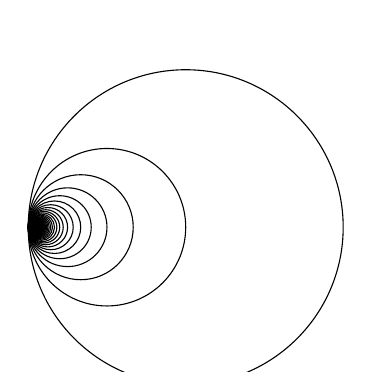
\begin{tikzpicture} 
        \foreach \n in {1,2,...,200} 
         \draw (2/\n,0) circle (2/\n);
       \end{tikzpicture}
    \end{center}
\end{zgled}

\subsection{Kvocientne preslikave}

Naj bo $f: X \to Y$. Kakšen mora biti $f$, da sploh določa inducirano preslikavo 
$\overline{f}: \quot{X}{\sim} \to Y$? Ker mora veljati $\overline{f}([x]) \mapsto f(x)$,
mora $f$ ekvivalentne točke v $X$ slikati v eno točko. Z drugimi besedami, $f$ mora biti konstantna v ekvivalenčnih razredih.

\begin{trditev}
    Veljajo naslednje trditve.
    \begin{itemize}
        \item Če za vsaka $x, y \in X$ velja $x \sim y \Rightarrow f(x) = f(y)$,
        potem $f$ določa inducirano preslikavo $\overline{f}: \quot{X}{\sim} \to Y$.
        \item Če je $f$ zvezna, je tudi $\overline{f}$ zvezna.
        \item Če je $f$ surjektivna, je tudi $\overline{f}$ surjektivna.
        \item $\overline{f}$ je injektivna, če za vsaka $x, y \in X$, ki nista v relaciji $\sim$, velja $f([x]) \neq f([y])$
        (tj. $f$ loči razrede).
    \end{itemize}
\end{trditev}

\begin{dokaz}
    Dokažimo drugo točko.
    Naj bo $\overline{f} : \quot{X}{\sim} \to Y$ in $V \subseteq Y$ odprta podmnožica.
    Potem je $q^{-1} (\overline{f}^{-1} (V)) = f^{-1} (V)$ in ker je $f$ zvezna, je $f^{-1} (V)$ odprta.
\end{dokaz}

Če je $f$ taka, da je $\overline{f}$ (zvezna) bijekcija, nas zanimajo dodatni pogoji, ki zagotavljajo,
da je $\overline{f}$ homeomorfizem, torej če $\overline{f}$ inducira bijekcijo med odprtimi 
množicami. Tako je poljubna množica $V \subseteq Y$ odprta natanko tedaj, ko je $\overline{f}^{-1} (V)$
odprta v $\quot{X}{\sim}$, to pa je natanko tedaj, ko je $f^{-1} (V)$ odprta v $Y$.

\begin{definicija}
  Funkcija $f: X \to Y$ je kvocientna, če je surjektivna in je vsaka množica $V \subseteq Y$
  odprta natanko tedaj, ko je $f^{-1} (V)$ odprta v $X$.
\end{definicija}

\begin{opomba}
  Surjektivna funkcija $f: X \to Y$ je kvocientna natanko tedaj, ko velja 
  \begin{equation}\label{eq:1}
    Z^{\, \mathrm{zap}} \subseteq Y \Leftrightarrow f^{-1} (Z)^{\, \mathrm{zap}} \subseteq X.
  \end{equation}
  V splošnem se kvocientna preslikava $f: X \to Y$ obnaša kot kvocientna projekcija glede na razčlenitev $X$
  na $f$-praslike točk iz $Y$. 
\end{opomba}

\begin{izrek}
  Naj bo $X$ topološki prostor z ekvivalenčno relacijo $\sim$ in $f: X \to Y$
  kvocientna preslikava, ki je konstantna na ekvivalenčnih razredih in jih med seboj loči 
  (pravimo, da naredi iste identifikacije kot $\sim$).
  Potem je $\overline{f}: \quot{X}{\sim} \to Y$ homeomorfizem.
\end{izrek}

\begin{lema}
  Naj bo $f: X \to Y$ zvezna in surjektivna. Če je $f$ še odprta ali zaprta, potem je kvocientna.
\end{lema}

\begin{dokaz}
  Dokažimo trditev za zaprto $f$, torej implikacijo \eqref{eq:1} v levo.
  Če je $Z \subseteq Y$ taka, da je $f^{-1} (Z)$ zaprta v $\quot{X}{\sim}$,
  potem je zaradi zaprtosti in surjektivnosti $f$ tudi $Z = f(f^{-1} (Z))$ zaprta v $Y$.
\end{dokaz}

\begin{opomba}
  Če je $X$ kompakt in $Y$ Hausdorffov, je zvezna preslikava $f: X \to Y$ takoj zaprta.
\end{opomba}

Označimo interval $I = [0, 1]$ in si oglejmo nekaj naravnih kvocientov kvadrata $I^2 = [0, 1]^2$.

\begin{zgled}
  Kvocientni prostor kvadrata $I^2$ z relacijo 
    $$\forall y \in I:\ (0, y) \sim (1, y)$$ je s funkcijo $$f: I^2 \to S^1 \times I,\ f(s, t) = (e^{2 \pi i s}, t)$$
    homeomorfen plašču valja.
    \begin{center}
      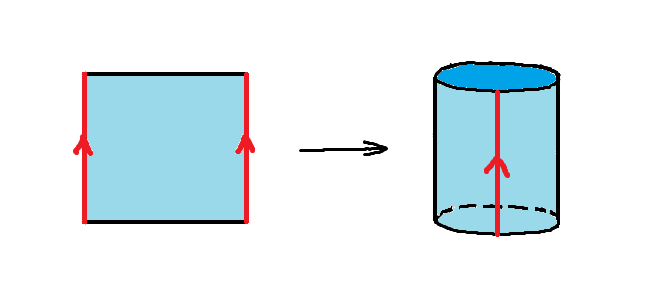
\includegraphics[scale=0.7]{zgled1.png}
    \end{center}
\end{zgled}

\begin{zgled}
  Möbiusov trak je kvocient kvadrata $I^2$ po relaciji $$\forall y \in I:\ (0, y) \sim (1, 1 - y).$$
  Ta prostor lahko vložimo v poln torus $S^1 \times B^2$ s preslikavo 
  $$f: I^2 \to S^1 \times B^2,\ (x, y) \mapsto (e^{2\pi i x}, e^{\pi i x} (2y - 1)),$$
  ki je očitno kvocientna.
  Poln torus $S^1 \times B^1$ pa lahko vložimo v $\R^3$ s predpisom 
  $$\varphi((x, y), (z, w)) = w(0, 0, 1) + (z + 2)(x, y, 0).$$
  Če sedaj $f$ komponiramo s $\varphi$, dobimo vložitev Möbiusovega traku 
  v $\R^3$.
  \begin{center}
    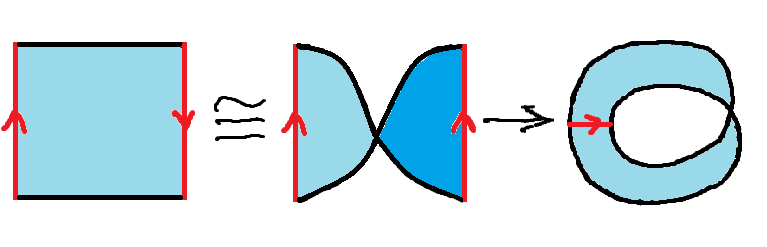
\includegraphics[scale=0.5]{zgled2.png}
  \end{center}
\end{zgled}

\begin{zgled}\label{zgl:2}
  Če kvadrat $I^2$ iz prejšnjih zgledov še enkrat zavihnemo in nato zlepimo robova,
  dobimo kvocientni prostor, homeomorfen kolobarju.
  \begin{center}
  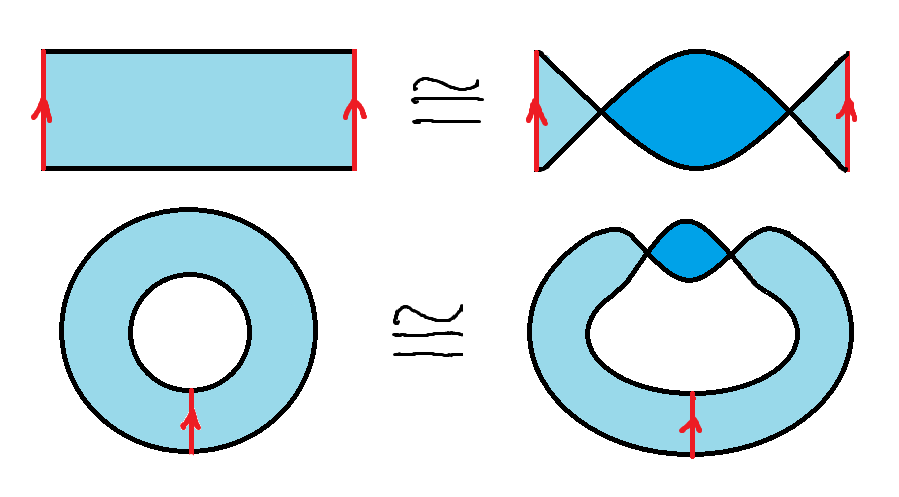
\includegraphics[scale=0.4]{zgled3.png}    
  \end{center}
  Z drugimi besedami, dobimo še eno vložitev 
  kvocienta kvadrata $I^2$ z relacijo 
  $(0, y) \sim (1, y)$ v $\R^3$.
\end{zgled}

\begin{zgled}\label{zgl:1}
  Na $B^2$ imamo ekvivalenčno relacijo, v kateri je edini netrivialni ekvivalenčni razred $S^1$:
    to lahko označimo kot $\quot{B^2}{S^1}$ in že intuitivno se zdi, da je ta prostor homeomorfen $S^2$.
    Možen predpis za kvocientno preslikavo $f: B^2 \to S^2$ bi bil
    $f(\vb{x}) = ((2 \sqrt{1 - \|\vb{x}\|^2}) \vb{x}, 2\|\vb{x}\|^2 - 1)$.
    \begin{center}
      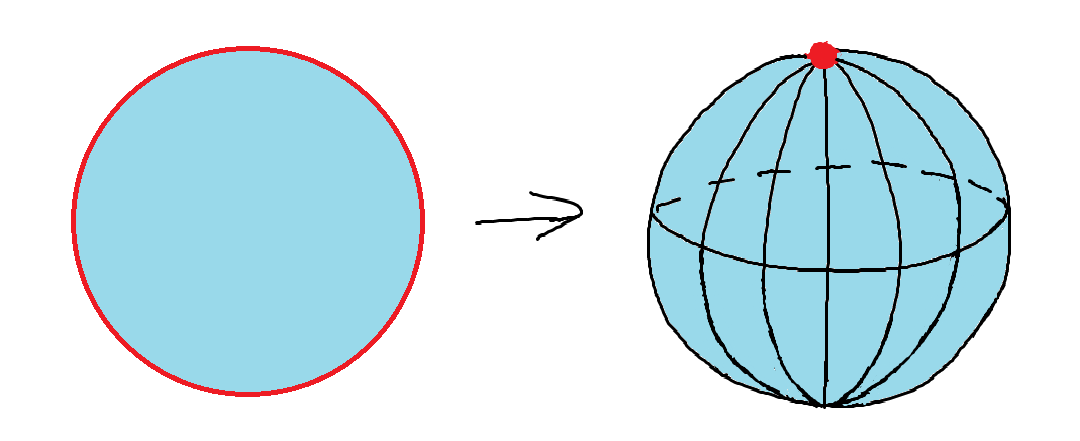
\includegraphics[scale=0.4]{zgled4.png}
    \end{center}
\end{zgled}

\begin{zgled}
  Kvocient kvadrata $I^2$ z relacijo 
  $$\forall x, y \in I:\ (0, y) \sim (1, y),\ (x, 0) \sim (x, 1)$$
  je homeomorfen torusu. Res, preslikava $$f: I^2 \to S^1 \times S^1,\ f(x, y) = (e^{2 \pi i x}, e^{2 \pi i y})$$
  je kvocientna in zato inducira homeomorfizem $\overline{f}: \quot{I^2}{\sim} \to S^1 \times S^1$.
  \begin{center}
    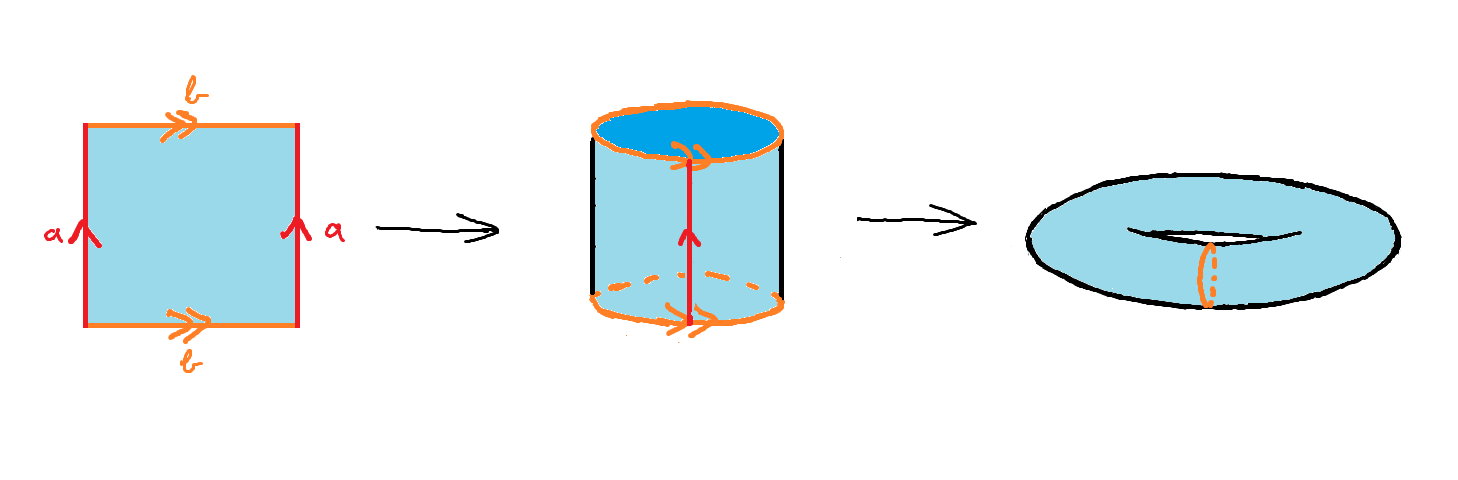
\includegraphics[scale=0.5]{zgled5.png}
  \end{center} 
\end{zgled}

\subsection{Operacije s kvocientnimi preslikavami}

\begin{trditev}
  Naj bosta $f: X \to Y$ in $g: Y \to Z$ funkciji.
  Potem velja:
  \begin{itemize}
    \item $f, g$ kvocientni $\Rightarrow$ $g \circ f$ kvocientna.
    \item $g \circ f$ kvocientna in $f, g$ zvezni $\Rightarrow$ $g$ kvocientna.
  \end{itemize}
\end{trditev}

\begin{dokaz}
  Dokažimo najprej prvo točko. Očitno je $g \circ f$ surjektivna in zvezna, zato je dovolj, da 
  preverimo lastnost \eqref{eq:1} v levo.
  \begin{align*}
    (g \circ f)^{-1} (V)^{\ \text{odp}} \subseteq X &\Rightarrow f^{-1} (g^{-1} (V))^{\ \text{odp}}\\
    &\Rightarrow g^{-1} (V)^{\ \text{odp}} \subseteq Y\\
    &\Rightarrow V^{\ \text{odp}} \subseteq Z.
  \end{align*}
  Pri drugi točki lahko takoj sklepamo, da je $g$ surjektivna in zvezna.
  Naj bo $V \subseteq Z$ taka, da je $g^{-1} (V)^{\ \text{odp}} \subseteq Y$. Potem sledi 
  \begin{align*}
    f^{-1} (g^{-1} (V))^{\ \text{odp}} \subseteq X &\Rightarrow (g \circ f)^{-1} (V) ^{\ \text{odp}}\\
    &\Rightarrow V^{\ \text{odp}} \subseteq Z. \qedhere
  \end{align*}
\end{dokaz}

\begin{zgled}
  Z uporabo prejšnje trditve lahko pokažemo, da je za $$A = S^1 \times \{1\} \cup \{1\} \times S^1 \subseteq S^1 \times S^1$$
  prostor $\quot{S^1 \times S^1}{A}$ homeomorfen sferi $S^2$.
  Res, označimo $B = \partial I^2$ in po zgledu \ref{zgl:1} je 
  $\quot{I^2}{B}$ homeomorfen $S^2$. Definirajmo še kvocientno preslikavo 
  $f: I^2 \to S^1 \times S^1$ kot $f(x, y) = (e^{2 \pi i x}, e^{2 \pi i y})$. 
  Sedaj pa naša predpostavka sledi iz prejšnje trditve:
  \adjustbox{scale=1.3,center}{
  \begin{tikzcd}
    I^2 \arrow[r, "f"] \arrow[d, "q_1"] \arrow[dr, "F = q_2 \circ f"]
      & S^1 \times S^1 \arrow[d, "q_2"] \\
    \quot{I^2}{B} \arrow[r, "\overline{F}"]
      &  \quot{S^1 \times S^1}{A},
  \end{tikzcd}
  }
  saj je $F = q_2 \circ f$ kvocientna.
\end{zgled}

\begin{opomba}
  Če je $h: X \to Y$ homeomorfizem in sta $\sim_X$ ter $\sim_Y$
  ekvivalenčni relaciji na $X$ oziroma $Y$, za kateri velja 
  $$x_1 \sim_X x_2 \Leftrightarrow h(x_1) \sim_Y h(x_2),$$
  potem je $\quot{X}{\sim} \cong \quot{Y}{\sim}$.
\end{opomba}

\subsection{Deljivost topoloških lastnosti}

\begin{definicija}
  Topološka lastnost $\mathcal{L}$ je deljiva, če se s poljubnega 
  topološkega prostora prenese na vsak njegov kvocientni prostor.
  To je ekvivalentno temu, da se $\mathcal{L}$ ohranja pri vsaki kvocientni preslikavi.
\end{definicija}

\begin{trditev}
  \begin{enumerate}
    \item Deljive topološke lastnosti so kompaktnost, povezanost (s potmi),
    diskretnost, trivialnost, separabilnost in lokalna povezanost (s potmi).

    \item Nedeljive topološke lastnosti so med drugim separacijske, lokalna kompaktnost,
    1-števnost, 2-števnost, metrizabilnost in popolna nepovezanost.
  \end{enumerate}
\end{trditev}

\begin{dokaz}
  \begin{enumerate}
    \item Večina od navedenih lastnosti velja zaradi ohranitve pri zveznih preslikavah.
    Dokažimo zato lokalno povezanost s potmi.
    Naj bo $f: X \to Y$ kvocientna in $X$ lokalno povezan s potmi.
    Potem so komponente vsake odprte množice odprte.
    Naj bo $V \subseteq Y$ odprta in $V = \cup_{\lambda \in \Lambda} V_\lambda$,
    kjer so $V_\lambda$ komponente $V$. Potem je $f^{-1} (V) = \cup_{\lambda \in \Lambda} f^{-1} (V_\lambda)$.
    Komponente $f^{-1} (V)$ so odprte v $X$, naj bo $W$ ena izmed teh komponent:
    $$f(W) \subseteq V \Rightarrow \exists \lambda_0 : f(W) \subseteq V_{\lambda_0} \Rightarrow W \subseteq f^{-1}(V_{\lambda_0}).$$
    Potem je $f^{-1} (V_\lambda)$ unija nekaj (odprtih) komponent množice $f^{-1} (V)$, zato je 
    $f^{-1} (V_\lambda)$ odprta v $X$ in ker je $f$ kvocientna, je $V_\lambda$ odprta v $Y$.
    
    \item Za razne topološke lastnosti podamo kar konkretne protiprimere.
    Za Hausdorffovo lastnost vzemimo $T_2$ prostor $X = \R \times \{0, 1\}$ z ekvivalenčno 
    relacijo $(x, 0) \sim (x, 1),\ \forall x \in (0, \infty)$.
    Za 1-števnost pa lahko na primer vzamemo 1-števen prostor $X = \N \times [0, 1]$, 
    definiramo $A = \N \times \{0\}$ in potem $\quot{X}{A}$ ni 1-števen. \qedhere
  \end{enumerate}
\end{dokaz}

Cantorjevo množico dobimo iz intervala $[0, 1]$, ki mu izbrišemo srednjo tretjino in nato ta postopek 
induktivno nadaljujemo. Tako dobimo Cantorjevo množico $C$, ki je metrični kompakt brez izoliranih točk 
in je povsem nepovezan.

\begin{opomba}
  Cantorjeva množica je homeomorfna prostoru funkcij $2^{\N}$,
  opremljenim s kompaktno-odprto topologijo, kjer je $2 = \{0, 1\}$
  diskreten prostor z dvema točkama.
\end{opomba}

\begin{figure}[htb!]
  \centering 
  \begin{tikzpicture}
    \foreach \order in {0,...,4}
      \draw[yshift=-\order*15pt]  l-system[l-system={cantor set, axiom=F, order=\order, step=250pt/(3^\order)}];
  \end{tikzpicture}
  \caption{Cantorjeva množica}
\end{figure}

\begin{izrek}
  Zgornje lastnosti določajo Cantorjevo množico do izomorfizma natančno.
\end{izrek}

\begin{izrek}[Aleksandrov]
  Če je $X$ poljuben metrični kompakt, obstaja zvezna surjekcija $f: C \to X$.
  Taka $f$ je tudi kvocientna.
\end{izrek}

Vzemimo metrični kompakt $X = I = [0, 1]$, to je torej kvocient Cantorjeve množice,
vendar pa je povezan, zato se popolna nepovezanost ne ohrani.
To bi lahko tudi dokazali tako, da uporabimo ekspliciten zapis Cantorjeve množice 
$$C = \{x = \sum_{i = 1} ^\infty \frac{2 x_i}{3^i}\ |\ x_i \in \{0, 1\}\}$$
in definiramo zvezno surjektivno preslikavo v $I$ s pomočjo dvojiškega zapisa:
$$f\left(\sum_{i = 1} \frac{2x_i}{3^i}\right) = \sum_{i = 1} \frac{x_i}{2^i}.$$

\begin{trditev}
  Naj bo $\mathcal{R}$ razčlenitev prostora $X$.
  Potem je $\quot{X}{\mathcal{R}} \in T_1$ natanko tedaj, ko so članice $\mathcal{R}$ zaprte v $X$.
\end{trditev}

\subsection{Topološke grupe in delovanja}

\begin{definicija}
  Topološka grupa $G$ je grupa $G$, ki je hkrati tudi topološki prostor, tako da sta strukturi povezani:
  \begin{itemize}
    \item množenje $G \times G \to G$ je zvezno.
    \item invertiranje $G \to G$ je zvezno.
  \end{itemize}
\end{definicija}

\begin{opomba}
  Poznamo že na primer topološko algebro zveznih funkcij ali pa $p$-adična števila.
  Ta je množica racionalnih števil, napolnjena v $p$-adični metriki. Naj bo $p$ praštevilo; 
  potem je 
  $$\left| \frac{m}{n} \right| = p^{-k},\ \mathrm{\text{če je $\frac{m}{n} = p^k \frac{a}{b}$ in sta $a, b$ tuji s $p$.}}$$
  S tem dobimo topološki obseg $p$-adičnih števil.
\end{opomba}

\begin{zgled}
  Navedimo nekaj zgledov topoloških grup.
  \begin{itemize}
    \item Poljubna grupa $G$, opremljena z diskretno topologijo je topološka grupa.
    \item Grupe $(\Q, +)$, $(\R, +)$, $(\C, +)$, $(\Ha, +)$ in pa tudi $(\R, \cdot)$, $(\C, \cdot)$, $(\Ha, \cdot)$
    so vse topološke grupe.
    \item Množice $S^0$, $S^1$ in $S^3$ so zaporedoma podgrupe topoloških grup $(\R, \cdot)$, $(\C, \cdot)$ in $(\Ha, \cdot)$
    ter so tudi same hkrati topološke podgrupe.
  \end{itemize}
\end{zgled}

\begin{zgled}
  Naj bo $\{G_\lambda\ |\ \lambda \in \Lambda\}$ družina topoloških grup.
  Potem definiramo $\prod_{\lambda \in \Lambda} G_\lambda$ kot direktni produkt grup 
  in topoloških prostorov z operacijo po komponentah:
  $$(g_\lambda)_{\lambda \in \Lambda} \cdot (h_\lambda)_{\lambda \in \Lambda} := (g_\lambda h_\lambda)_{\lambda \in \Lambda}.$$
  Na tej množici vpeljemo produktno topologijo. Preprost primer je, če proglasimo 
  $G_n \cong \Z_2$ za vsak $n \in \N$. Potem je 
  $$\prod_{n \in \N} G_n = \Z_2^{\N} \cong C\ \ldots\ \textup{Cantorjeva množica}.$$
\end{zgled}

\begin{zgled}
  Oglejmo si nekatere topološke grupe linearnih izomorfizmov.
  Naj bo $\mathbb{F}$ topološki obseg, torej $\mathbb{F} \in \{\R, \C, \Ha\}$.
  Naj bo $V$ $n$-dimenzionalni vektorski prostor nad $\mathbb{F}$, torej 
  $V \cong \mathbb{F}^n$ s produktno topologijo. Naj bo $\mathrm{GL}(V)$
  množica vseh linearnih izomorfizmov $V \to V$.
  Potem lahko $V$ identificiramo s $\mathbb{F}^n$, torej je 
  $$\mathrm{GL}_n \mathbb{F} = \{A \in \mathbb{F}^{n \times n}\ |\ \det A \neq 0\}^{\ \textup{odp}} \subseteq \mathbb{F}^{n \times n}\quad \textup{z evklidsko topologijo.}$$
  Splošna linearna grupa je topološka grupa. Res, množenje je očitno zvezno,
  saj sestoji iz elementarnih funkcij; enako velja tudi za invertiranje.
  Podobno sledi za naslednje grupe:
  \begin{itemize}
    \item $\mathrm{SL}_n \F = \{A \in \mathrm{GL}_n \F\ |\ \det A = 1\}$,
    \item $\mathrm{O}_n = \{A \in \mathrm{GL}_n (\R)\ |\ A A^\top = I\}$,
    \item $\mathrm{SO}_n = \mathrm{SL}_n \R \cap \mathrm{O}_n$,
    \item $\mathrm{U}_n = \{A \in \mathrm{GL}_n (\C)\ |\ A A^\mathsf{H} = I\}$,
    \item $\mathrm{SU}_n = \mathrm{U}_n \cap \mathrm{SL}_n \C$.
  \end{itemize}
\end{zgled}

\begin{opomba}
  To so primeri Liejevih grup; tako pravimo topološkim grupam,
  ki so hkrati gladke mnogoterosti in v katerih so operacije gladke preslikave.
\end{opomba}

\begin{trditev}
  Naj bo $G$ topološka grupa in $a \in G$. Potem je leva translacija za $a$,
  definirana kot $$L_a : G \to G,\quad g \mapsto ag$$
  homeomorfizem.
\end{trditev}

\begin{opomba}
  Enako velja za desno translacijo $a$, torej $D_a : G \to G$, $g \mapsto ga$.
\end{opomba}

\begin{dokaz}
  Leva translacija $L_a : G \to G$ je zvezna, saj je kompozitum zveznih funkcij
  $$G \to \{a\} \times G,\ g \mapsto (a, g) \quad \mathrm{in} \quad \{a\} \times G \to G,\ (a, g) \mapsto ag.$$
  Inverz $L_a$ je $L_{a^{-1}}$, saj je $L_a \circ L_{a^{-1}} = \mathrm{Id}$.
  Od tod pa sledi dokaz trditve.
\end{dokaz}

\begin{posledica}
  Topološka grupa $G$ je homogen prostor, torej za poljubna $a, b \in G$
  obstaja homeomorfizem $h: G \to G$, da je $h(a) = b$.
\end{posledica}

\begin{dokaz}
  Definiramo $h := L_{b^{-1}a}$.
\end{dokaz}

\begin{definicija}
  Naj bo $X$ topološki prostor in $G$ topološka grupa, potem je (levo)
  delovanje grupe $G$ in prostora $X$ zvezna preslikava $\varphi: G \times X \to X$,
  za katero velja 
  \begin{itemize}
    \item $e \cdot x = x,\ \forall x \in X$.
    \item $a \cdot (b \cdot x) = (ab) \cdot x,\ \forall a, b \in G,\ \forall x \in X$.
  \end{itemize}
  Topološki prostor $X$ z delovanjem $G$-grupe imenujemo $G$-prostor.
\end{definicija}

\begin{opomba}
  Za vsak $a \in G$ je $\varphi(a, \cdot): X \to X$ leva funkcija za $a$, ki je homeomorfizem.
  Ampak v splošnem $X$ ni homogen prostor, saj za poljubni izbrani točki ne obstaja nujno translacija, ki preslika eno v drugo.
\end{opomba}

\begin{trditev}
  Delovanje grupe $G$ na $X$ določa ekvivalenčno relacijo na $X$:
  $$x \sim y \Leftrightarrow \exists g \in G,\ y = g \cdot x.$$
\end{trditev}
\vspace*{-3mm}
Ekvivalenčne razrede imenujemo orbite: orbita točke $x$ je 
$$G \cdot x := \{g \cdot x\ |\ g \in G\} \subseteq X.$$
Orbite tvorijo particijo prostora $X$. Prostor $\quot{X}{\sim} := \quot{X}{G}$
imenujemo prostor orbit\footnote[1]{Pri tem moramo paziti, da razlikujemo med podobnim zapisom, kjer
bi črka $G$ označevala netrivialni ekvivalenčni razred. Razliko med zapisom razberemo iz konteksta.}.
Za poljuben $x \in X$ imenujemo 
$$G_x := \{ g \in G\ |\ gx = x\} \leq G.$$
stabilizatorska podgrupa. Iz algebre že vemo, da obstaja bijekcija med $G \cdot x$ in $\quot{G}{G_x}$. 

\begin{zgled}
  Če je $G$ topološka grupa in $H \leq G$ podgrupa, potem je tudi $H$ topološka grupa.
  Zožitev množenja v $G$ določa delovanje $H$ na $G$:
  $$H \times G \to G,\quad (h, g) \mapsto hg.$$
  Takšen primer je recimo delovanje $\Z$ na $\R$ s translacijami za cela števila:
  $$Z \times \R \to \R,\quad (a, x) \mapsto x + n.$$
  Orbita točke $x$ je $x + \Z = \{x + n\ |\ n \in \Z\} = [x]$.
  Pokazali bomo, da je prostor orbit $\quot{\R}{\Z}$ homeomorfen $\quot{[0, 1]}{0 \sim 1}$,
  ta pa je nadalje homeomorfen $S^1$.
  \adjustbox{scale=1.5,center}{
    \begin{tikzcd}
        \R \arrow[r, "f"] \arrow[d, "q"] 
          & S^1\\
        \quot{\R}{\Z} \arrow[ur, dashed, "\overline{f}"]
          &  
    \end{tikzcd}
  }
  Definirajmo $f: \R \to S^1$, $f(x) = e^{2\pi i x}$. Očitno je $f$ surjektivna in zvezna
  ter naredi iste identifikacije kot $\Z$:
  $$f(x) = f(y) \Leftrightarrow e^{2 \pi i x} = e^{2 \pi i y} \Leftrightarrow x = y + k,\ k \in \Z.$$
  Dovolj bi bilo že, če bi dokazali, da je $f$ zaprta. To pa ni res, saj se množica 
  $$A = \{n + \frac{1}{2^n}\ |\ n \in \N\}^{\ \textup{zap}} \subseteq \R,$$
  ne preslika v zaprto množico, ker v njeni sliki ni elementa $1 \in S^1$.
  Na srečo pa $f$ je odprta, saj vsak odprt interval $U \subseteq \R$ dolžine manj kot $1$ 
  injektivno preslika na odprt lok v krožnici. Torej je $\overline{f}$ homeomorfizem. 
\end{zgled}

\begin{zgled}
  Množica $S^1 \subseteq \C$ je topološka grupa in deluje na 
  $\C$ z množenjem kompleksnih števil:
  $$S_1 \times \C \to \C,\quad (\alpha, z) \mapsto \alpha z.$$
  Prostor orbit $\quot{\C}{S^1}$ je izomorfen $[0, \infty)$.
\end{zgled}

\begin{zgled}
  Naj bo $\F \in \{ \R, \C, \Ha\}$, torej je $\F^*$ topološka grupa 
  za množenje z evklidsko topologijo. Potem $\F^*$ deluje na 
  $\F^n$ z množenjem s skalarji:
  $$\F^* \times \F^n \to \F^n,\quad (\lambda, v) \mapsto \lambda v.$$
  Orbita vektorja $\vb{v} \in \F^n$ je $\F$-premica skozi 
  $\vb{v}$ brez izhodišča, ničelni element pa je kar sam svoja orbita.
\end{zgled}

\begin{trditev}
  Naj bo $G$ topološka grupa, ki deluje na topološki prostor $X$.
  Potem je kvocientna projekcija $q: X \to \quot{X}{G}$ odprta.
\end{trditev}

\begin{dokaz}
  Za poljubno odprto množico $V \subseteq X$ moramo pokazati, da je njeno nasičenje 
  $q^{-1} (q(V))$ odprto.
  \begin{align*}
    q^{-1} (q(V)) &= \{y\ |\ y \sim x\ \text{za nek $x \in V$}\}\\
    &= \{g \cdot x\ |\ x \in V,\ g \in G\}\\
    &= \bigcup_{g \in G} \{g \cdot x\ |\ x \in V\}\\
    &= \bigcup_{g \in G} g\cdot V {=} \bigcup_{g \in G} L_g (V)^{\ \text{odp}},
  \end{align*}
  ker je $L_g$ homeomorfizem.
\end{dokaz}

\subsection{Konstrukcije kvocientov}

\begin{enumerate}
  \item \textbf{Stožec}
\end{enumerate}

Naj bo $X$ topološki prostor in $I = [0, 1]$. Potem kvocientu 
  $$CX := \quot{X \times I}{X \times \{1\}}.$$
  pravimo stožec nad $X$.
  \begin{center}
    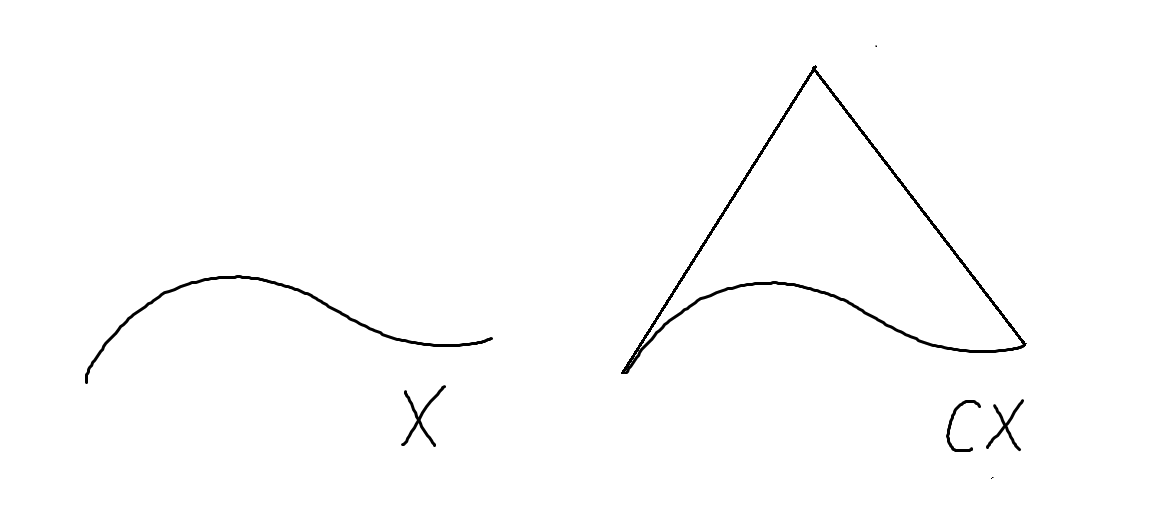
\includegraphics[scale=0.4]{stozec.png}
  \end{center}

\begin{enumerate}
  \setcounter{enumi}{1}
  \item \textbf{Suspenzija} 
\end{enumerate}

Suspenzija nad $X$ je kvocient 
  $$\Sigma X := \quot{X \times [-1, 1]}{X \times \{-1\}, X\times \{1\}}.$$

\begin{opomba}
  Če je $X \subseteq \R^n$ in obstaja $c \in \R^n$,
  da se daljice $[c, x]$, $x \in X$ sekajo paroma le v $c$,
  potem unijo teh daljic imenujemo linearni stožec.
  Če je $X$ kompakt, ima njegov linearni stožec enake 
  topološke lastnosti kot $CX$.
\end{opomba}

\begin{trditev}
  $CS^n \cong B^{n + 1}$ in $\Sigma S^n \cong S^{n + 1}$.
  \begin{center}
    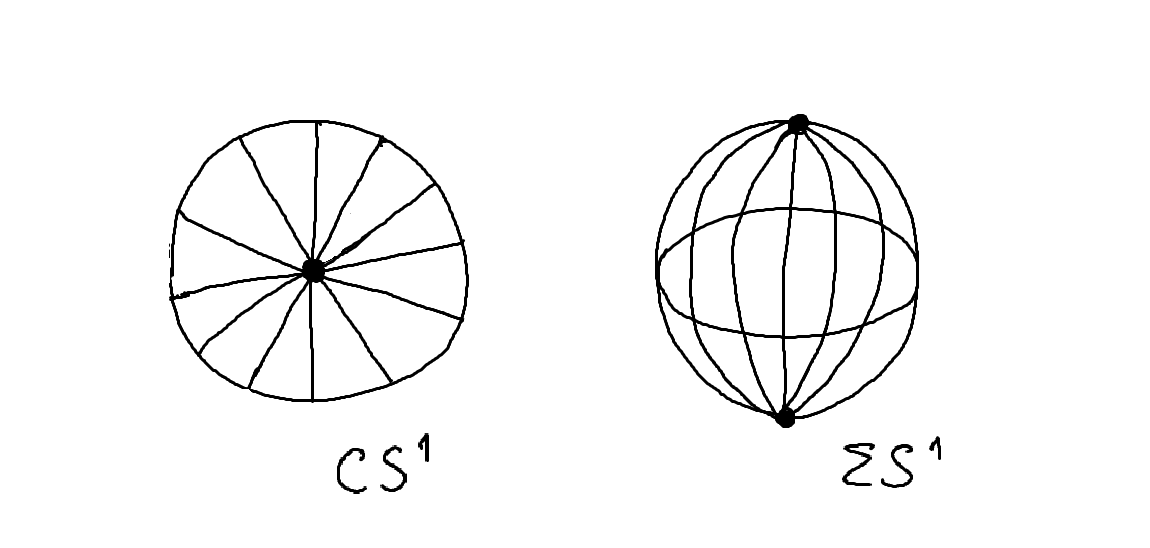
\includegraphics[scale=0.4]{trditev1.png}
  \end{center}
\end{trditev}

\begin{enumerate}
  \setcounter{enumi}{2}
  \item \textbf{Simetrični produkt} 
\end{enumerate}

  Simetrični produkt je množica vseh neurejenih $n$-teric;
  če je $X$ topološki prostor, $n \in \N$ in $X^n = \{x_1, \dots, x_n)\ |\ x \in X\}$,
  potem definiramo 
  $$S^n X := \quot{X^n}{S_n},$$
  kjer je $S_n$ simetrična grupa, ki deluje s permutacijami.

\begin{enumerate}
  \setcounter{enumi}{3}
  \item \textbf{Limita prostorov} 
\end{enumerate}

  Limita prostorov $X_1 \stackrel{f_1}{\to} X_2 \stackrel{f_2}{\to} X_3 \stackrel{f_3}{\to} X_4 \cdots$
  je definirana kot $$\lim_{\rightarrow} (X_n, f_n) := \quot{\bigsqcup_{n = 1}^\infty}{\sim},$$
  kjer za $x \in X_i$ in $y \in X_j$ vpeljemo relacijo 
  $$x \sim y \Leftrightarrow \exists n \in \N:\ f_n (\cdots f_{i + 1} (f_i (x))) = f_n (\dots f_{j + 1} (f_j (y))).$$

\begin{enumerate}
  \setcounter{enumi}{4}
  \item \textbf{Zlepek prostorov}
\end{enumerate}

Naj bosta $X$ in $Y$ topološka prostora $A \subseteq X$ in $f: A \to Y$.
  Potem je zlepek $X$ in $Y$ vzdolž $f$ kvocient 
  $$X \cup_f Y := \quot{(X \bigsqcup Y)}{a \sim f(a), \forall a \in A}.$$
  Njegovi ekvivalenčni razredi so $[x] = \{x\}$ za $x \in X \setminus A$,
  $[y] = \{y\}$ za $y \in Y \setminus f(A)$ in pa $[y] = \{y\} \cup f^{-1}(\{y\})$ za $y \in f(A)$.
  \begin{center}
    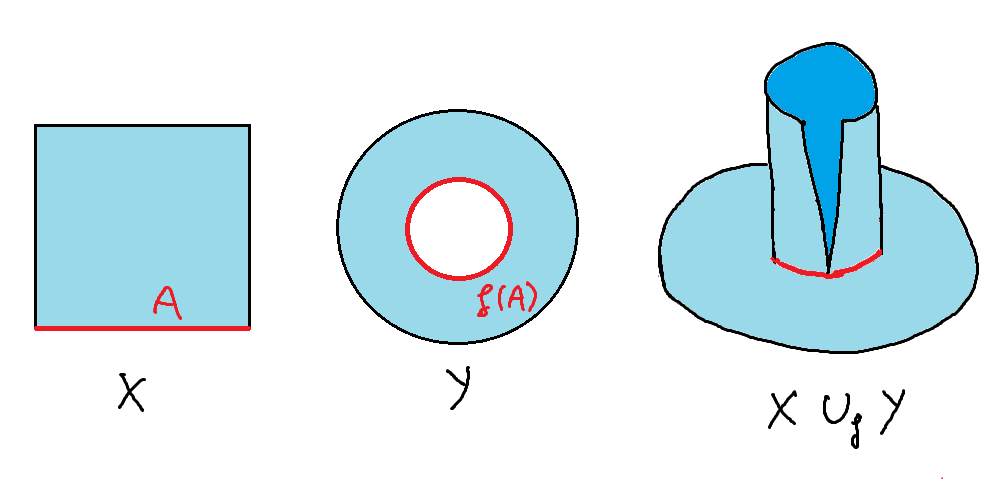
\includegraphics[scale=0.5]{zlepek.png}
  \end{center}

\begin{zgled}
  Navedimo nekaj primerov zlepkov.
  \begin{itemize}
    \item Če je $A \subseteq X$, potem je $\quot{X}{A}$ zlepek za preslikavo 
    $f: A \to Y = \{*\}$, torej je v tem primeru $X \cup_f Y \cong \quot{X}{A}$.
    \item Če je $f: S^{n-1} \to S^{n-1}$ homeomorfizem, potem je $B^n \cup_f B^n \cong S^n$.
    \item Preslikavni valj preslikave $f: X \to Y$ je zlepek $X \times I$ in $Y$,
    ki $X \times \{0\}$ z $f$ prilepi na $Y$.
  \end{itemize}
\end{zgled}

\begin{izrek}
  Naj bosta $X$ in $Y$ normalna prostora, $A^{\ \text{zap}} \subseteq X$
  in $f: A \to Y$ zvezna. Potem je $X \cup_f Y$ normalen.
\end{izrek}

\begin{dokaz}
  Lastnost $T_1$ sledi zato, ker so ekvivalenčni razredi zaprti;
  res, za $y \in f(A)$ je $[y] = \{y\} \cup f^{-1} (\{y\})$ unija dveh zaprtih množic.
  Dokažimo še lastnost $T_4$, in sicer z Urisonovo karakterizacijo.
  Prostor $Z$ je $T_4$, če za poljubni disjunktni zaprti množici $B, C \subseteq Z$
  obstaja Urisonova funkcija $\varphi: Z \to I$, da je $\varphi \big|_B = 0$
  in $\varphi \big|_{C} = 1$.
  V $X \cup_f Y$ izberemo poljubni disjunktni zaprti množici $B, C$.
  Naj bo $q: X \sqcup Y \to X \cup_f Y$ kvocientna projekcija in 
  $$B_X := q^{-1} (B) \cap X, \ B_Y := q^{-1} (B) \cap Y, \ C_X := q^{-1} (C) \cap X, \ C_Y := q^{-1} (C) \cap Y.$$
  Potem sta $B_X, C_X^{\quad \text{zap}} \subseteq X$ disjunktni in enako tudi za 
  $B_Y, C_Y^{\quad \text{zap}} \subseteq Y$.
  Ker je $Y \in T_4$, obstaja Urisonova funkcija $\varphi_y : Y \to I$,
  tako da je $\varphi_y \big|_{B_Y} = 0$ in $\varphi_y \big|_{C_Y} = 1$. 
  To določa funkcijo $\psi : A \cup B_X \cup C_X \to I$,
  $$\psi (x) := \begin{cases}
    \varphi_y (f(x)); & x \in A\\
    0;& x \in B_X\\
    1;& x \in C_X
  \end{cases}.$$
  Ta predpis je zvezen, saj je zvezen na lokalno končnem zaprtem pokritju
  in se predpisi na presekih ujemajo. Po Tietzejevem razširitvenem izreku
  obstaja razširitev $\varphi_X : X \to I$ za funkcijo $\psi$, saj je 
  množica $A \cup B_X \cup C_X$ zaprta v $X$. Sedaj pa $\varphi_Y$ in $\varphi_X$
  določata iskano Urisonovo funkcijo na $X \cup_f Y$.
  \begin{center}
    \adjustbox{scale=1.3,center}{
    \begin{tikzcd}
      X \sqcup Y \arrow[r, "\varphi_X \sqcup \varphi_Y"] \arrow[d, "q"]
        & I \\
      \quot{X}{\sim} \arrow[ur, dashed, "\varphi"]
        & 
    \end{tikzcd}}  
  \end{center}
  Preslikava $\varphi_X \sqcup \varphi_Y$ je po konstrukciji zvezna, hkrati pa je tudi 
  konstantna na ekvivalenčnih razredih:
  $$y \in f(A):\ \{y\} \cup f^{-1} (y),\ \varphi_X (x) = \varphi_Y (f(x)) = \varphi_Y (y).$$
  Očitno je tudi $\varphi\big|_B = 0$ in $\varphi\big|_C = 0$, saj je po konstrukciji 
  \begin{equation*}
    \varphi_X \sqcup \varphi_Y \big|_{q^{-1} (B)} = 0, \quad \varphi_X \sqcup \varphi_Y \big|_{q^{-1} (C)} = 1. \qedhere
  \end{equation*}
\end{dokaz}

\begin{trditev}\label{trd:1}
  Naj bo $A^{\,\text{zap}} \subseteq X$, $f: A \to Y$ zaprta vložitev in $Z = X \cup_f Y$.
  \begin{enumerate}
    \item Če sta $X, Y$ 2-števna, je $Z$ 2-števen.
    \item Če sta $X, Y \in T_2$, je tudi $Z \in T_2$. 
  \end{enumerate}
\end{trditev}

\begin{dokaz}
  Naj bo $\mathcal{B}_X = \{U_n\ |\ n \in \N\}$ števna baza za $X$ in 
  $\mathcal{B}_Y = \{V_n\ |\ n \in \N\}$ števna baza za $Y$.
  Označimo $$U_n \cap A \cap f^{-1} (V_m) =: W_{n, m}^{\ \text{odp}} \subseteq A.$$
  Če je $W_{n, m} \neq \emptyset$, potem obstaja odprta množica ${W_{n, m} }^X \subseteq U_n$,
  da je ${W_{n, m} }^X \cap A = W_{n, m}$.
  \begin{center}
    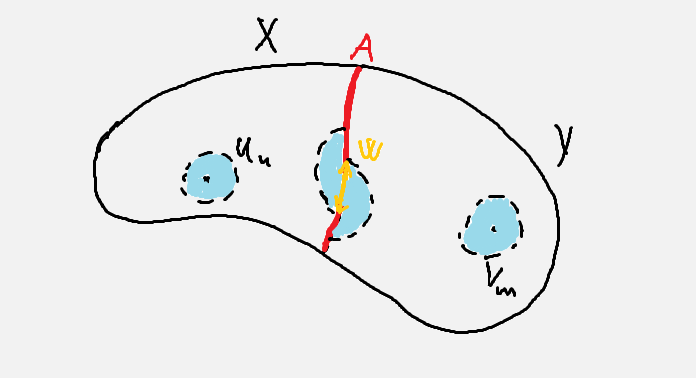
\includegraphics[scale=0.6]{dokaz1.png}
  \end{center}
  Podobno seveda tudi obstaja odprta množica ${W_{n, m} }^Y \subseteq V_m$,
  da je $f^{-1}({W_{n, m} }^Y) \cap A = W_{n, m}$.
  Sedaj označimo $U_n', V_m'$ kot bazne množice v $X$ oziroma $Y$, ki ne sekajo $A$ oziroma 
  $f(A)$. To so nasičene odprte množice, saj sekajo le trivialne ekvivalenčne razrede.
  Torej so $q(U_n'), q(V_m')^{\ \text{odp}} \subseteq Z$.
  Za poljubno $W_{n, m} \neq \emptyset$ pa je ${W_{n, m} }^{X} \sqcup {W_{n, m} }^{Y}$
  odprta in nasičena, saj po konstrukciji velja 
  $$x \in A:\ x \in {W_{n, m} }^{X} \sqcup {W_{n, m} }^{Y} \Leftrightarrow f(x) \in {W_{n, m} }^{X} \sqcup {W_{n, m} }^{Y}.$$
  Torej imamo podano števno družino odprtih množic v $Z$ s predpisom 
  \begin{align*}
    \mathcal{B} &= \{q(U_n')\ |\ U_n' \in \mathcal{B}_X,\ U_n' \cap A = \emptyset\}\\
    &\cup \{q(V_m')\ |\ V_m' \in \mathcal{B}_Y,\ V_m' \cap f(A) = \emptyset\}\\
    &\cup \{q({W_{n, m} }^{X} \sqcup {W_{n, m} }^{Y})\ |\ W_{n, m} \neq \emptyset\}.
  \end{align*}
  Dokazati moramo še, da je $\mathcal{B}$ tudi baza.
  Za vsako $O^{\ \text{odp}} \subseteq Z$ in poljubno $z \in O$ moramo 
  pokazati, da obstaja $B \in \mathcal{B}$, da je $z \in B \subseteq O$.
  Vemo, da je $$q^{-1} (z) \subseteq q^{-1} (O)^{\ \text{odp}} \subseteq X \sqcup Y.$$
  Če je $z \notin q(A)$, potem je bodisi $q^{-1} (z) \in X \setminus A$ ali pa $Y \setminus f(A)$.
  Dovolj je, če se omejimo na prvi primer; tedaj je $z \in q^{-1} (O) \cap (X \setminus A)^{\ \text{odp}} \subseteq X$.
  Potem pa že obstaja $U_n \in \mathcal{B}_X$, da je $q^{-1}(z) \in U_n \subseteq q^{-1} (O) \cap (X \setminus A)$.
  Če pa je $z = [a] = [f(a)]$ za nek $a \in A$, potem je 
  $a \in q^{-1} (O) \cap X^{\ \text{odp}}$ in zato obstaja nek $U_n$,
  da je $a \in U_n \subseteq q^{-1} (O) \cap X$. Po enakem premisleku obstaja $V_m$,
  da je $f(a) \in V_m \subseteq q^{-1} (O) \cap Y$. Vemo tudi, da $W_{n,m} = U_n \cap A \cap f^{-1}(V_m) \neq \emptyset$.
  Torej je $$z = [a] \in q({W_{n, m} }^X \sqcup {W_{n, m} }^Y) \subseteq O$$
  in smo končali.
  \begin{center}
    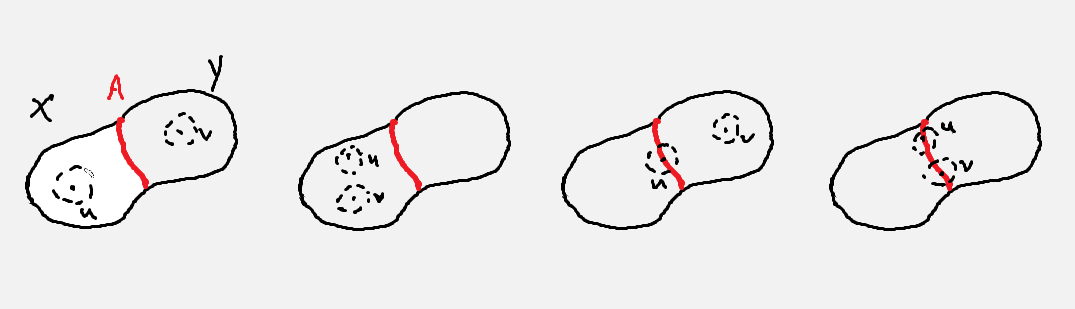
\includegraphics[scale=0.75]{dokaz2.png}
  \end{center}
  Sedaj dokažimo še drugo točko. Omejimo se na primer, ko je 
  $u = [a] = [f(a)]$ in $v = [b] = [f(b)]$ za $a \neq b,\ a, b \in A$.
  Potem obstajata disjunktni odprti okolici $U_1, U_2 \subseteq X$ za $a, b$
  in disjunktni odprti okolici $V_1, V_2 \subseteq Y$ za $f(a), f(b)$.
  Označimo 
  $$W_1 := U_1 \cap A \cap f^{-1} (V_1),\ W_1 := U_1 \cap A \cap f^{-1} (V_2)$$
  in kot v dokazu prve konstruiramo disjunktni odprti okolici 
  $$q({W_1 }^{X} \sqcup {W_1 }^{Y}),\ q({W_2 }^{X} \sqcup {W_2 }^{Y})$$
  točk $[a]$ in $[b]$.
\end{dokaz}

\subsection{Projektivni prostori}

\textbf{Motivacija}: v ravninski geometriji nastopita dve možni 
(različni) medsebojni legi dveh različnih premic; premici sta si vzporedni ali 
pa se sekata v natanko eni točki. V izogib temu želimo geometrijo,
kjer bo situacija za dve poljubni premici enaka.

Preprosto povedano to naredimo tako, da vsakemu snopu vzporednih premic "`dodamo točko v neskončnosti"'.
Formalno pa to definiramo na naslednji način.

\begin{definicija}
  Naj bo $\F \in \{\R, \C, \Ha\}$ in $n \in \N_0$.
  Projektivni prostor dimenzije $n$ nad $\F$ je 
  $$\F P^n := \quot{(\F^{n + 1} \setminus\{0\})}{(x = \lambda x,\ \lambda \in \F^*)} =  \quot{(\F^{n + 1} \setminus \{0\})}{\F^*}.$$
\end{definicija}

\begin{opomba}
  Enako lahko naredimo za poljuben topološki obseg, na primer za $\Z_p$ z diskretno topologijo 
  ali pa za $p$-adična števila.
\end{opomba}

\begin{trditev}
  $\F P^n$ je homogen prostor: za poljubni točki $u, v \in \F P^n$
  obstaja homeomorfizem $h: \F P^n \to \F P^n$, tako da je $h(u) = v$.
\end{trditev}

\begin{dokaz}
  Naj bo $u = [\vb{x}]$ in $v = [\vb{y}]$.
\begin{center}
  \adjustbox{scale=1.3,center}{
    \begin{tikzcd}
      \F^{n + 1} \setminus \{0\} \arrow[r, "H"] \arrow[d, "q"] \arrow[dr, "q \circ H"]
        & \F^{n + 1} \setminus \{0\} \arrow[d, "q"] \\
      \F P^n \arrow[r, dashed, "h"]
        & \F P^n
    \end{tikzcd}
  }  
\end{center}
Vektor $\vb{x}$ dopolnimo do baze $\vb{x}, \vb{x_1}, \dots, \vb{x_n}$,
vektor $\vb{y}$ pa do $\vb{y}, \vb{y_1}, \dots, \vb{y_n}$.
Naj bo $P$ prehodna matrika, da je $P \vb{x} = \vb{y}$.
Naj bo $$H : \F^{n + 1} \setminus\{0\} \to \F^{n + 1} \setminus \{0\}$$
zožitev pripadajoče linearne preslikave, ki je tudi bijektivna in je zato homeomorfizem,
torej kvocientna preslikava.
Zato je tudi $q \circ H$ kvocientna.
Ker $H$ slika premice v premice, slika ekvivalenčne razrede v ekvivalenčne razrede za $q$,
torej $q \circ H$ naredi iste identifikacije kot $q$. To pa že pomeni, da je inducirana preslikava $h$
homeomorfizem in 
\begin{equation*}
  h(u) = h(q(\vb{x})) = q(H(\vb{x})) = q(\vb{y}) = v. \qedhere
\end{equation*}
\end{dokaz}

\begin{zgled}
  Navedimo nekaj trivialnih primerov projektivnih prostorov.
  \begin{itemize}
    \item $\F P^0 = \quot{\F^1 \setminus \{0\}}{\F^*} = \quot{\F^*}{\F^*} = \{a\}$.
    \item $\F P^1 = \quot{\F^2 \setminus \{0\}}{\F^*}$, tako dobimo $\R P \cong S^1$, $\C P \cong S^2$ in $\Ha P \cong S^4$.
    \item $\R P^2$ je tudi ploskev, ki pa morda v nasprotju za našimi pričakovanji 
    ni homoemorfen prostoru $S^2$.
  \end{itemize}
\end{zgled}

Cilj tega razdelka je poenostaviti opis projektivnega prostora, da bi bolje 
razumeli topološke lastnosti, kot so na primer kompaktnost.
Takoj lahko za prostor $\R^{n + 1} \setminus\{0\}$ podamo trivialno opazko,
da vsaka premica skozi izhodišče seka enotsko sfero,
zato so predstavniki vseh ekvivalenčnih razredov $\R P^n$
zaprti v kompaktni sferi.

\begin{comment}
  \begin{figure}[htb!]
  \centering
  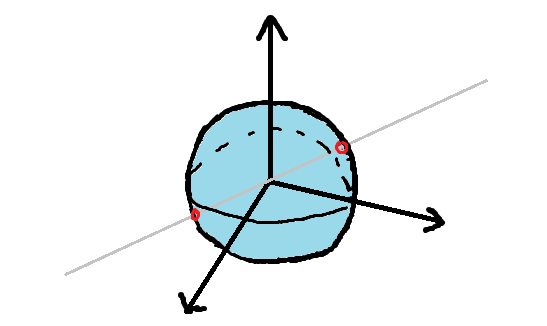
\includegraphics[scale=0.6]{projektivna2.png}
\end{figure}
\end{comment}
Najprej omenimo, da je $\F \in \{\R, \C, \Ha\}$ normiran obseg, torej za normo 
$\| \cdot \|$ v $\F$ velja $\| x \cdot y\| = \|x\| \|y\|$.
Hkrati iz lastnosti norme sledi, da lahko le enotski skalarji ohranjajo enotsko sfero.
Tako delovanje grupe $\F^*$ porodi delovanje grupe enotskih skalarjev na enotski sferi.

\begin{definicija}
  Naj bo $\F \in \{\R, \C, \Ha\}$ in $n \in \N_0$.
  Potem definiramo $S(\F^n) := \{\vb{x} \in \F^n\ |\ \| \vb{x}\| = 1\}$.
\end{definicija}

\begin{opomba}
  $S(\R^n) = S^{n - 1}$, $S(\C^n) = S^{2n - 1}$ in $S(\Ha ^n) = S^{4n - 1}$.
\end{opomba}

\begin{trditev}
  \begin{enumerate}
    \item Kvocientna projekcija $q: \F^{n + 1} \setminus\{0\} \to \F P^n$ je odprta.
    \item $\F P^n \cong \quot{S(\F^{n + 1})}{S(\F)}$.
    \item $\F P^n$ je kompakten, lokalno kompakten, povezan s potmi, lokalno povezan s potmi in 2-števen. 
  \end{enumerate}  
\end{trditev}

\begin{dokaz}
  Dokažimo drugo točko.
  \begin{center}
    \adjustbox{scale=1.3,center}{
      \begin{tikzcd}
        \F^{n + 1} \setminus\{0\} \arrow[r, "r"] \arrow[d, "q"] \arrow[dr, "p \circ r"]
          & {S(\F^{n + 1})} \arrow[d, "p"] \\
        \F P^n \arrow[r, dashed]
          & \quot{S(\F^{n + 1})}{S(\F)}
      \end{tikzcd}
    }  
  \end{center}
  Vpeljimo $r(\vb{x}) = \frac{\vb{x}}{\| \vb{x}\|}$ in dokažimo, da je kvocientna.
  Očitno je zvezna in surjektivna. Dokazujemo, da je še odprta.
  Upoštevamo, da je $\F^{n + 1} \equiv \R^k$, torej $r$ slika iz $\R^k \setminus \{0\}$ 
  v $S^{n - 1}$. Potem je $r$ kompozitum homeomorfizma in projekcije.
  \begin{align*}
    \R^k \setminus \{0\} \stackrel{h}{\to} &S^{k - 1} \times (0, \infty) \stackrel{\mathrm{pr}_1}{\to} S^{k - 1}\\
    \vb{x}  \mapsto &\left(\frac{\vb{x}}{\| \vb{x} \|}, \| \vb{x}\|\right) \mapsto \frac{\vb{x}}{\| \vb{x}\|}.
  \end{align*}
  Ker sta homeomorfizem in projekcija odprti, je tudi $r$ odprta in zato je $p \circ r$ kvocientna.
  Če $p \circ r$ naredi iste identifikacije kot $q$, je inducirana preslikava homeomorfizem.
  Preverimo najprej v eno smer:
  \begin{align*}
    (p \circ r) (\vb{x}) = (p \circ r) (\vb{y}) &\Leftrightarrow p\left(\frac{\vb{x}}{\|\vb{x}\|}\right) = p\left(\frac{\vb{y}}{\|\vb{y}\|}\right)\\
    &\Leftrightarrow \frac{\vb{x}}{\|\vb{x}\|} = \lambda \cdot \frac{\vb{y}}{\|\vb{y}\|},\ \lambda \in S(\F)\\
    &\Rightarrow \vb{y} = \lambda \frac{\| \vb{y}\|}{\|\vb{x}\|} \vb{x}\\
    &\Rightarrow q (\vb{y}) = \vb{x}.
  \end{align*}
  Obratno; če je $q(\vb{y}) = q(\vb{x})$, potem obstaja $\mu \in \F^*$, $\vb{y} = \mu \vb{x}$.
  $$\| \vb{y} \| = \|\mu\| \cdot \|\vb{x}\|$$
  Od tod pa sledi $\| \mu \| = \frac{\|\vb{y}\|}{\| \vb{x}\|}$ in končno 
  $$\vb{y} = \mu \vb{x} = \frac{\mu}{\| \mu \|} \frac{\|\vb{y}\|}{\|\vb{x}\|} \vb{x},$$
  kjer je $\frac{\mu}{\| \mu \|} \in S(\F)$ in zato res $(p \circ r) (\vb{x}) = (p \circ r) (\vb{y}).$
\end{dokaz}

\begin{posledica}
  $\R P^{n} \cong \quot{S^n}{S^0} \cong \quot{S^n}{\{1, -1\}} = \quot{S^n}{x \sim -x}$.
\end{posledica}

\begin{center}
  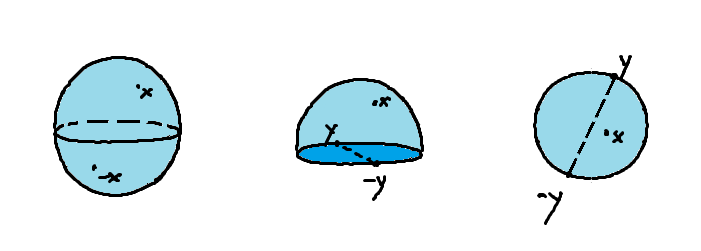
\includegraphics[scale=0.8]{projektivna3.png}
\end{center}

\begin{trditev}
  \begin{itemize}
    \item $\R P^n \cong \quot{B^n}{y \sim -y,\ y \in S^{n - 1}}$
    \item $\C P^n \cong \quot{B^{2n}}{y \sim \lambda y,\ y \in S^{2n - 1},\ \lambda \in S^1}$
    \item $\Ha P^n \cong \quot{B^{4n}}{y \sim \lambda y,\ y \in S^{4n - 1},\ \lambda \in S^3}$
  \end{itemize}
\end{trditev}

\begin{dokaz}
  Preverimo le prvo točko, saj drugi dve sledita analogno.
  \begin{center}  
  \adjustbox{scale=1.1,center}{
      \begin{tikzcd}
        B^n \arrow[r, "h"] \arrow[d, "q"] \arrow[drr, "f"]
          & S^n_+ \arrow[hookrightarrow, r, "i"] 
          & S^n \arrow[d, "p"]\\
        \quot{B^n}{y \sim -y,\ y \in S^{n - 1}} \arrow[rr, dashed, "\overline{f}"]
        & 
          & \quot{S^n}{\{1, -1\}}
      \end{tikzcd}
    }
    \end{center}   
    Funkcija $f$ je zvezna, kvocientna (točke na $S_+ ^n$ sekajo vse ekvivalenčne razrede za $p$)
    in zaprta, kar bomo sedaj dokazali. Dovolj je že če dokažemo, da je $p \circ i$
    zaprta. Naj bo $A \subseteq S_+ ^n$ zaprta; ker je $i$ zaprta vložitev (${S_+ ^n} ^{\ \text{zap}} \subseteq S^n$),
    je dovolj pokazati, da je $p(i(A)) = p(A)$ zaprta. Vemo pa že, da je to natanko tedaj,
    ko je $p^{-1} (p (A))^{\ \text{zap}} \subseteq S^n$, kar pa seveda drži.
    Nazadnje moramo pokazati še, da $f$ naredi iste identifikacije kot $q$:
    \begin{gather*}
      x \in \inte\, B^n \implies f^{-1} (f(x)) = \{x\}\\
      x \in S^{n - 1} \implies f^{-1} (f(x)) = \{x, -x\}. \qedhere
    \end{gather*}
\end{dokaz}

\begin{zgled}
  $\R P^{2} \cong \quot{S^2}{\{1, -1\}} = \quot{B^2}{x \sim -x,\ x \in S^1}$.
  \begin{center}
    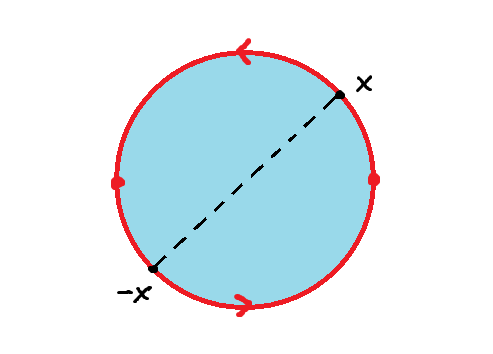
\includegraphics[scale=0.6]{zgled6.png}
  \end{center}
\end{zgled}

\clearpage
\section{Osnovni izreki topologije evklidskih prostorov}

\subsection{Brouwerjev izrek o negibni točki}

\begin{definicija}
  Preslikava $f: X \to X$ ima negibno točko $c \in X$,
  če je $f(c) = c.$ 
\end{definicija}

Obstoj negibne točke je odvisen tako od lastnosti prostora kot od lastnosti preslikave.

\begin{zgled}
  Banachovo skrčitveno načelo pove, da ima skrčitev $f: X \to X$ na polnem metričnem prostoru
  $X$ negibno točko.
\end{zgled}

Naslednji izjavi pravimo Brouwerjev izrek o negibni točki.

\begin{trditev}[\textbf{Izjava $\mathbf{A_n}$}]
  Vsaka zvezna preslikava $f: B^n \to B^n$ ima negibno točko.
\end{trditev}

\begin{opomba}
  Za $n = 1$ ta izrek poznamo že iz analize 1.
  Res, naj bo zvezna preslikava $f: [-1, 1] \to [-1, 1]$.
  Da negibna točka te preslikave obstaja, sledi iz izreka o vmesni vrednosti 
  za funkcijo $g(x) = f(x) - x$.
  \begin{center}
    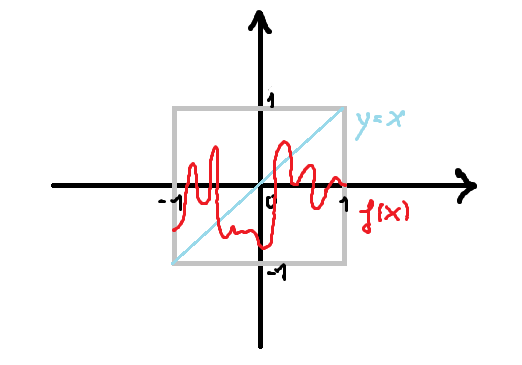
\includegraphics[scale=0.7]{opomba1.png}
  \end{center}
\end{opomba}

\begin{zgled}
  Za $B^n \setminus \{0\}$ ta izrek ne velja. Protiprimer je kar funkcija $f: B^n \setminus \{0\} \to B^n \setminus \{0\}$ 
  s predpisom $f(x) = -x$.
\end{zgled}

\begin{definicija}
  Topološki prostor $X$ ima lastnost negibne točke (LNT),
  če ima vsaka zvezna preslikava $f: X \to X$ negibno točko.
\end{definicija}

\begin{opomba}
  LNT je topološka lastnost, torej se ohranja s homeomorfizmi.
\end{opomba}

\begin{definicija}
  $A \subseteq X$ je retrakt prostora $X$, če obstaja retrakcija $r: X \to A$,
  torej zvezna preslikava $r$, ki je na $A$ identiteta.
  \begin{center}
    \adjustbox{scale=1.3,center}{
      \begin{tikzcd}
        A \arrow[hookrightarrow, d, "i"] \arrow[dr, "id"]
          & \\
        X \arrow[r, dashed, "r"]
          & A
      \end{tikzcd}
    }  
  \end{center}
\end{definicija}

\begin{zgled}
  Navedimo nekaj osnovnih primerov retraktov.
  \begin{itemize}
    \item $X$ je sam svoj retrakt, saj ima retrakcijo $r = id$.
    Hkrati pa je za poljuben $x_0 \in X$ tudi enojec $\{x_0\}$ retrakt prostora $X$.
    V tem primeru moramo seveda vzeti konstantno preslikavo $r(x) = x_0,\ \forall x \in X$.
    \item $S_+ ^n$ je retrakt sfere $S^n$ za retrakcijo 
    $$r(x_1, \dots, x_n, x_{n + 1}) = (x_1, \dots, x_n, |x_{n + 1}|).$$
    \item Ali obstaja retrakcija intervala $[-1, 1]$ na $A = \{-1, 1\}$? Odgovor je negativen,
    saj mora biti zvezna slika povezanega prostora $[-1, 1]$ prav tako povezana.
  \end{itemize}
\end{zgled}

\begin{lema}
  Če ima $X$ LNT in je $Y \subseteq X$ njegov retrakt, ima tudi $Y$ LNT.
\end{lema}

\begin{dokaz}
  Naj bo $r: X \to Y$ retrakcija in $f: Y \to Y$ poljubna zvezna preslikava.
  Definirajmo preslikavo $g$:
  $$g: X \stackrel{r}{\to} Y \stackrel{f}{\to} Y \stackrel{i}{\hookrightarrow} X.$$
  Ker ima $X$ lastnost negibne točke, obstaja tak $x_0 \in X$, da je $g(x_0) = x_0$.
  Torej je $i(f(r(x_0))) = x_0$, od koder pa naprej sledi $f(r(x_0)) = x_0$.
  Ker pa mora biti $x_0 \in Y$, je $r(x_0) = x_0$ in imamo $f(x_0) = x_0$,
  kar smo želeli dokazati.
\end{dokaz}

\begin{trditev}
  \begin{itemize}
    \item Retrakt povezanega prostora je povezan prostor.
    \item Retrakt kompaktnega prostora je kompakten.
    \item Če je $X \in T_2$ in je $A \subseteq X$ retrakt, je $A ^{\ \text{zap}} \subseteq X$.
  \end{itemize}
\end{trditev}

\begin{dokaz}
  Dokažimo tretjo točko.
  Naj bo $r: X \to A$ retrakcija. Potem se zvezni preslikavi 
  $id: X \to X$ in $f: X \stackrel{r}{\to} A \stackrel{i}{\hookrightarrow} X$
  ujemata na $A$, od koder po Hausdorffovi lastnosti sledi zaprtost $A$.
\end{dokaz}

\begin{trditev}
  Retrakcija ohranja lokalno povezanost (s potmi) in lokalno kompaktnost.
\end{trditev}

\begin{dokaz}
  Dokažimo za lokalno povezanost. Ta je ekvivalentna temu, da je povezana komponenta vsake odprte množice prav tako odprta.
  Naj bo $X$ lokalno povezan prostor in $r: X \to A$ retrakcija. Naj bo $N^{\ \text{odp}} \subseteq A$ in $C$ njena komponenta. 
  Nato izberemo točko $x \in C$. Ker je retrakcija zvezna, je $r^{-1} (N) ^{\ \text{odp}} \subseteq X$.
  Zaradi lokalne kompaktnosti je $x$ vsebovan v odprti komponenti $U \subseteq r^{-1} (N)$.
  Ker je zvezna slika povezanega prostora povezana, velja $r(U) \subseteq C$.
  Od tod pa dobimo $$x \in U \cap A \subseteq r(U) \subseteq C$$
  in ker je $U^{\ \text{odp}} \subseteq X$, je $x \in U \cap A ^{\ \text{odp}} \subseteq C$.
  To pa že pomeni, da je komponenta $C$ odprta.
\end{dokaz}

\begin{izrek}[Tietze]
  Naj bo $X$ normalen prostor, $A ^{\ \text{zap}} \subseteq X$, $J$ realen interval in 
  zvezna preslikava $f: A \to J$. Potem obstaja razširitev $F: X \to J$ za $f$, torej
  $F\big|_A = f$.
  \begin{center}
    \adjustbox{scale=1.3,center}{
      \begin{tikzcd}
        A^{\ \text{zap}} \arrow[r, "f"] \arrow[hookrightarrow, d, "i"] 
          & J \\
        X \arrow[ur, dashed, "F"]
          & 
      \end{tikzcd}
    }  
  \end{center}
\end{izrek}

\begin{definicija}
  $Y$ je absolutni ekstenzor za nek razred $\mathcal{R}$ topoloških prostorov,
  če za vsak $X \in \mathcal{R}$, vsako $A^{\ \text{zap}} \subseteq X$
  in vsako zvezno preslikavo $f: A \to Y$ obstaja zvezna preslikava $F: X \to Y$,
  da je $F \big|_A = f$, torej da je $F$ razširitev $f$ na $X$.
\end{definicija}

\begin{opomba}
  To označujemo $Y \in AE(\mathcal{R})$. Tietzejev izrek nam pove,
  da je vsak interval $J$ vsebovan v $AE (\mathcal{N})$, kjer $\mathcal{N}$
  označuje razred normalnih prostorov.
\end{opomba}

\begin{trditev}
  \begin{enumerate}
    \item Vsebovanost v $AE(\mathcal{R})$ je topološka lastnost.
    \item Če je $Y_\lambda \in AE(\mathcal{R})$ za vse $\lambda \in \Lambda$, potem je tudi $\prod_{\lambda \in \Lambda} Y_\lambda \in AE(\mathcal{R})$.
    \item Če je $Y \in AE(\mathcal{R})$ in je $Z$ retrakt $Y$, potem je $Z \in AE(\mathcal{R})$.
  \end{enumerate}
\end{trditev}

\begin{dokaz}
  Dokažimo tretjo točko. Naj bo $r: Y \to Z$ retrakcija. Izberimo poljuben podprostor 
  $A^{\ \text{zap}} \subseteq X \in \mathcal{R}$ in zvezno preslikavo $f: A \to Z$.
  \begin{center}
    \adjustbox{scale=1.5,center}{
      \begin{tikzcd}
        A \arrow[r, "f"] \arrow[hookrightarrow, d, "i"'] \arrow[dr, "j \circ f"']
          & Z \arrow[hookrightarrow, d, shift right=0.50ex, "j"'] \\
        X \arrow[r, dashed, "\exists G"']
          & Y \arrow[u, shift right=0.75ex, "r"']
      \end{tikzcd}
    }  
  \end{center}  
  Označimo $g = j \circ f$ in imamo po predpostavki njeno razširitev $G: X \to Y$.
  Potem je razširitev od $f$ kar $F = r \circ G$. 
  To je res, saj je 
  \begin{equation*}
    F \big|_A = r \circ G\big|_A = r \circ g = r \circ j \circ f = f. \qedhere
  \end{equation*}
\end{dokaz}

\begin{definicija}
  $Y$ je absolutni retrakt za neki razred topoloških prostorov $\mathcal{R}$,
  če je $Y \in \mathcal{R}$ in velja, da če za $X$ obstaja zaprta vložitev $\varphi: Y \to X$,
  potem je $\varphi(Y)$ je retrakt za $X$.
\end{definicija}

\begin{zgled}
  Za vsako točko velja $\{ *\} \in AR (\mathcal{R})$.
\end{zgled}

\begin{trditev}
  $\mathcal{R} \cap AE(\mathcal{R}) \subseteq AR(\mathcal{R})$
\end{trditev}

\begin{posledica}
  Poljuben interval $J$ je vsebovan v $AR (\mathcal{N})$.
\end{posledica}

\begin{dokaz}
  Naj bo $Y \in \mathcal{R} \cap AE(\mathcal{R})$. Izberemo poljuben $X \in \mathcal{R}$
  in poljubno zaprto vložitev $\varphi : Y \to X$.
  Označimo $\varphi(Y) =: A^{\ \textrm{zap}} \subseteq X$.
  Ker je $Y \in AE (\mathcal{R})$, je $A \in AE(\mathcal{R})$.
  Iščemo retrakcijo $r: X \to A$, torej zvezno preslikavo, ki je identiteta na $A$.
  \begin{center}
    \adjustbox{scale=1.3,center}{
      \begin{tikzcd}
        A \arrow[r, "id"] \arrow[hookrightarrow, d, "i"'] 
          & A \in AE(\mathcal{R}) \\
        X \in \mathcal{R} \arrow[ur, dashed, "\exists r"']
          & 
      \end{tikzcd}
    }  
  \end{center}   
  Iz diagrama pa vidimo, da taka $r$ obstaja po konstrukciji.
\end{dokaz}

\begin{trditev}[\textbf{Izjava $\mathbf{B_n}$}]
  $S^{n - 1}$ ni retrakt $B^n$.
\end{trditev}

\begin{zgled}
  Vemo že, da to ne velja za primer $n = 1$, saj $S^0 = \{-1, 1\}$ ni retrakt $B^1 = [-1, 1]$.
  Tudi v primeru $n = 2$ se intuitivno zdi, da če bi obstajal retrakt $r: B^2 \to S^1$, 
  bi se disk $B^2$ moral vmes nekje pretrgati.
  Vsekakor pa lahko preboden disk retraktiramo na $S^1$, in sicer z retrakcijo $r = \frac{x}{\|x\|}$.
\end{zgled}

Za tretjo ekvivalentno formulacijo Brouwerjevega izreka potrebujemo pojem homotopije, torej zvezne deformacije
preslikav.

\begin{definicija}
  \begin{enumerate}
    \item Zvezni preslikavi $f, g : X \to Y$ sta homotopni $(f \simeq g)$, če med njima obstaja homotopija 
    oziroma zvezna preslikava $H: X \times I \to Y$, za katero velja $H(x, 0) = f(x)$ in $H(x, 1) = g(x)$.
    \item Prostor $X$ je kontraktibilen, če je $id_X$ homotopna kakšni konstantni preslikavi.
    Takšni homotopiji pravimo kontrakcija.
  \end{enumerate}
\end{definicija}

\begin{figure}[htb!]
  \centering
  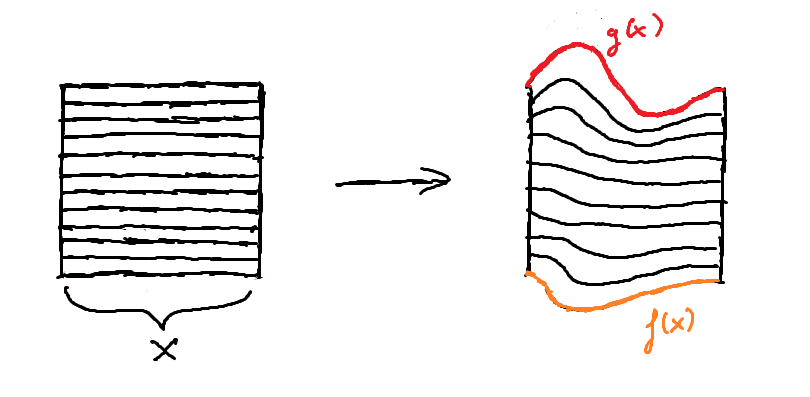
\includegraphics[scale=0.6]{homotopija1.png}
  \caption{Homotopija med funkcijama $f, g: X \to Y$}
\end{figure}

\begin{opomba}
  \begin{itemize}
    \item Kontrakcija cel prostor zvezno deformira v točko.
    Kontrakcija ima za končno preslikavo retrakcijo v eno točko.
    Čeprav je točka vedno retrakt, pa vsak prostor ni kontraktibilen.
    \item Homotopijo $H: X \times I \to Y,\ (x, t) \mapsto H(x, t)$ včasih označujemo kot preslikavo 
    $H_t(x)$, tako da je $H_t: X \to Y,\ H_t (x) = H(x, t)$. Če je $H$ homotopija od $f$ do $g$,
    je torej $H_0 = f$ in $H_1 = id$.
    \item Homotopnost je ekvivalenčna relacija.
  \end{itemize}
\end{opomba}

  Naj bosta $X, Y$ prostora in naj ima $\mathcal{C} (X, Y)$ kompaktno-odprto topologijo.
  Če je $f: X \times Z \to Y$ zvezna, enako velja tudi za inducirano preslikavo $F: Z \to \mathcal{C} (X, Y)$.
  Obratno velja, če je $X$ lokalno kompakten in Hausdorffov. To je posplošitev trditve,
  da je homotopija prostorov $X$ in $Y$ ekvivalentna poti v $\mathcal{C}(X, Y)$ pri določenih predpostavkah\footnote[2]{glej: Munkres, J.: Topology}.

\begin{zgled}
  Naj bo $X$ poljuben prostor in naj bosta poljubni zvezni preslikavi $f, g : X \to B^n$.
  Potem sta $f$ in $g$ homotopni, saj imamo homotopijo $$H(x, t) = (1 - t) f(x) + t g(x).$$
  Enako velja, če $B^n$ zamenjamo s poljubno konveksno podmnožico $\R^n$.
  \begin{center}
    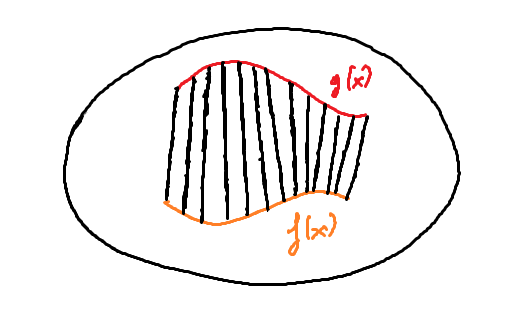
\includegraphics[scale=0.7]{zgled7.png}
  \end{center}  
  Tako prostori so potemtakem tudi kontraktibilni: primer kontrakcije prostora $\R^n$ v izhodišče je 
  $$H(x, t) = (1 - t)x.$$
\end{zgled}

\begin{zgled}
  Ali je $S^0 = \{-1, 1\}$ kontraktibilen? Denimo, da imamo kontrakcijo 
  $$H: S^0 \times I \to S^0,\ H_0 = id_{S^0},\ H_1 = c.$$
  Ker je $H(-1, 0) = \{-1\}$, se mora interval $\{-1\} \times I$ (povezana množica)
  preslikati v $-1$. Podobno se mora $\{1\} \times I$ preslikati v $\{1\}$.
  To pa pomeni, da je $H_1 = id_{S^0}$ in pridemo v protislovje.
\end{zgled}

\begin{trditev}[\textbf{Izjava $\mathbf{C_n}$}]
  Sfera $S^{n - 1}$ ni kontraktibilna.
\end{trditev}

\begin{trditev}
  Kontraktibilen prostor je povezan s potmi.
\end{trditev}

\begin{dokaz}
  Če je $X$ kontraktibilen, obstaja homotopija $H$ od $id_X$ do konstantne preslikave $g(x) = x_0$
  za neko točko $x_0 \in X$. Izberimo poljubni točki $x, y \in X$ in naj bo $c_x (t) = H(x, t)$
  pot od $x$ do $x_0$. Analogno naj bo $c_y (t) = H(y, t)$ pot od $y$ do $y_0$.
  Sedaj pa definiramo pot $c: I \to X$ kot 
  \begin{equation*}
    c(t) := \begin{cases}
      c_x (2t) ;& 0 \leq t \leq \frac{1}{2}\\
      c_y (2 - 2t) ;& \frac{1}{2} \leq t \leq 1.
    \end{cases} \qedhere
  \end{equation*} 
\end{dokaz}

\begin{izrek}
  Za vsak $n \in \N$ so izjave $\mathbf{A_n}$, $\mathbf{B_n}$ in $\mathbf{C_n}$ ekvivalentne.
\end{izrek}

\begin{dokaz}
  $(\mathbf{A_n} \Rightarrow \mathbf{B_n})$ Denimo, da obstaja retrakcija $r: B^n \to S^{n - 1}$.
  Pokazati moramo, da obstaja zvezna funkcija $f: B^n \to S^{n - 1}$ brez negibnih točk.
  $$B^n \stackrel{r}{\to} S^{n - 1} \stackrel{i}{\hookrightarrow} B^n$$
  Definiramo $g: B^n \to B^n$ s predpisom $g(x) = -x$ in $f = g \circ r : B^n \to B^n$.
  Ta preslikava pa nima negibne točke, saj bi iz $f(x) = x$ sledilo $(g(r(x))) = x$,
  to pa pomeni, da je $r(x) = -x \in S^{n -1}$. To pa je protislovje z definicijo retrakcije.

  $(\mathbf{B_n} \Rightarrow \mathbf{A_n})$ Denimo, da $\mathbf{A_n}$ ne velja, torej obstaja zvezna preslikava 
  $f: B^n \to B^n$, ki nima negibne točke. Iščemo retrakcijo $r: B^n \to S^{n - 1}$.
  Za vsak $x \in B^n$ je $f(x) \neq x$, zato točki $x$ in $f(x)$ enolično določata premico.
  \begin{center}
    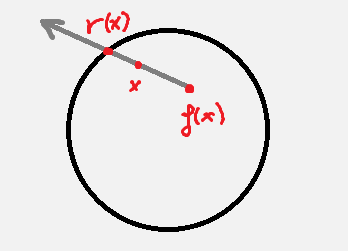
\includegraphics[scale=0.9]{dokaz3.png}
  \end{center}
  Označimo z $R(x)$ odprt poltrak te premice iz $f(x)$ skozi $x$. Presečišče $r(x) = R(x) \cap S^{n -1}$
  določa sliko retrakcije $r$. Za $r: B^n \to S^{n - 1}$ je treba še preveriti, če je zvezna in sploh dobro definirana.
  To je razvidno iz njenega predpisa:
  $$r(x) = f(x) + \frac{\sprod{f(x)}{f(x) - x} + \sqrt[]{(1 - \sprod{x}{f(x)})^2 - (1 - \|x\|^2)(1 -\|f(x)\|^2)}}{\|x - f(x)\|^2}(x - f(x)).$$ 
  Očitno pa je, da velja $r\big|_{S^{n -1}} = id\big|_{S^{n - 1}}$.

  $(\mathbf{B_n} \Rightarrow \mathbf{C_n})$ Denimo, da obstaja kontrakcija $S^{n - 1}$,
  torej $$H : S^{n - 1} \times I \to S^{n - 1},\quad H_0 = id_{S^{n -1}},\quad H_1 = c.$$
  Definirajmo funkcijo 
  $$f: S^{n - 1} \times I \to B^n,\quad (x, t) \mapsto (1-t)x.$$
  Ta preslikava je zvezna, surjektivna in zaprta, torej je kvocientna.
  \begin{center}
    \adjustbox{scale=1.5,center}{
      \begin{tikzcd}
        S^{n - 1} \times I \arrow[r, "H"] \arrow[d, "f"']
          & S^{n - 1} \\
        B^n \arrow[ur, dashed, "r"']
          & 
      \end{tikzcd}
    }  
  \end{center}  
  Edini netrivialni ekvivalenčni razred, določen z $f$, je $S^{n -1} \times \{1\}$, kjer je $H$ 
  konstanta, torej $H$ določa zvezno inducirano pot $r: B^n \to S^{n -1}$.
  \begin{center}
    \adjustbox{scale=1.5,center}{
      \begin{tikzcd}
        (x, 0) \arrow[mapsto, r, "H"] \arrow[mapsto, d, "f"']
          & x \in S^{n -1}\\
        x \in B^n \arrow[mapsto, ur, dashed, "r"']
          & 
      \end{tikzcd}
    }  
  \end{center} 
  $(\mathbf{C_n} \Rightarrow \mathbf{B_n})$ Denimo, da obstaja retrakcija $r: B^n \to S^{n - 1}$.
  Pokazati želimo, da obstaja kontrakcija sfere $S^{n - 1}$. Potem definiramo $f$ tako kot zgoraj 
  in dobimo želeno $H = r \circ f$.
\end{dokaz}

Preostane nam še pokazati, da so vse tri izjave $\mathbf{A_n}$, $\mathbf{B_n}$ in $\mathbf{C_n}$ tudi resnične.
Dokazali bomo izjavo $\mathbf{C_n}$ za primer $n = 2$.
Dokazati torej želimo, da identična preslikava krožnice sama vase ni 
homotopna nobeni konstantni preslikavi. Osnovna ideja dokaza je, da 
identična preslikava enkrat obhodi krožnico, konstantna pa ne.
V ta namen bomo definirali ovojno število poti. Kompleksno ravnino bomo identificirali 
z $\R^2$, parametrizacijo sklenjene krivulje $\Gamma$ v ravnini 
pa bomo gledali kot preslikavo $\gamma : [0, 1] \to \C$.
Ker zaradi sklenjenosti krivulje $\Gamma$ velja $\gamma(0) = \gamma (1)$, lahko parametrizacijo 
ekvivalentno obravnavamo kot preslikavo $g: S^1 \to \C$, pri čemer gledamo $S^1 \cong \quot{[0, 1]}{0 \sim 1}$.
Definiramo $$\varphi: [0, 1] \to S^1,\ \varphi(t) = e^{2 \pi i t}$$
in imamo zvezo $\gamma = g \circ \varphi$.

\begin{definicija}
  Ovojno število preslikave $g: S^1 \to \quot{\C}{\{0\}}$, ki opiše krivuljo $\Gamma = g(S^1)$, glede na izhodišče 
  je 
  $$w(g) = \frac{1}{2 \pi i} \int_{\Gamma} \frac{dz}{z} = \frac{1}{2 \pi i} \int_0 ^1 \frac{\gamma'(t)}{\gamma(t)}\, dt.$$
\end{definicija}

Primitivna funkcija za zadnji integral je kompleksni logaritem 
$$\log \gamma(t) = \log |\gamma(t)| + i \arg \gamma(t).$$
Oglejmo si najprej realni del. Takoj lahko vidimo, da se prispevka pri 
$t = 0$ in $t = 1$ odštejeta, saj sta dolžini enaki.
Drugače pa je z argumentom, ki se lahko pri večih obhodih
krivulje okoli izhodišča spremeni za nek celoštevilski večkratnik 
polnega kota $2 \pi$. Kompleksni logaritem je večlična funkcija in 
da dobimo primitivno funkcijo, moramo izbrati njene vrednosti vzdolž krivulje 
$t \mapsto \gamma(t)$ tako, da bo $t \mapsto \log(\gamma(t))$ zvezna.
Od tod vidimo, da je ovojno število krivulje celo število.

\begin{zgled}
  Ovojno število konstantne preslikave $$g: S^1 \to S^1,\ g(z) = a$$
  za neki $a \in \C \setminus \{0\}$, je enako $0$.
\end{zgled}

\begin{zgled}
  Naj bo $n \in \Z$ ter $g_n : S^1 \to \C$ podana z $g_n(z) = z^n$.
  V skladu z dogovorom izberemo parametrizacijo $\gamma_n(t) = e^{2 n \pi i t}$.
  Potem je $\gamma_n '(t) = 2 n \pi i \gamma_n (t)$, zato je 
  $$w (g_n) = \int_0 ^1 n\, dt = n.$$
  Od tod tudi sledi, da je ovojno število identične preslikave enako 1.
\end{zgled}

Izrek $\mathbf{C_2}$ bomo dokazali tako, da pokažemo, da je imata 
homotopni preslikavi enaki ovojni števili -- ovojno število je torej 
invarianta homotopskega razreda preslikave.
Najprej to preverimo za gladke homotopije.

\begin{lema}
  Naj bo $G: S^1 \times [0, 1] \to \C \setminus \{0\}$ gladka preslikava, ki je homotopija med 
  $G_0 = G(\cdot , 0)$ in $G_1 = G(\cdot , 1)$. Potem je $w (G_0) = w (G_1)$.
\end{lema}

\begin{dokaz}
  Za vsak $s \in [0, 1]$ označimo $G_s := G(\cdot, s)$in $\Gamma_s = G_s (S^1)$.
  Pokazati želimo, da je ovojno število $w(s) = w(G_s)$ neodvisno od $s \in [0, 1]$
  Ker je interval povezan in ovojno število zavzame le celoštevilske vrednosti,
  je dovolj pokazati, da je funkcija $s \mapsto w(s)$ zvezna. To pa sledi iz lastnosti 
  integrala s parametrom. Kot zgoraj naj bo 
  $$\widetilde{\gamma} (t, s) = G(e^{2 \pi i t}, s) = G_s (e^{2 \pi i t}).$$
  Tako definirana funkcija $\widetilde{\gamma}: [0, 1]^2 \to \C \setminus \{0\}$ je seveda zvezno odvedljiva,
  zato je 
  $$w(s) = \frac{1}{2 \pi i} \int_{\Gamma_s} \frac{dz}{z} = \frac{1}{2 \pi i} \int_0 ^1 \frac{\frac{\partial}{\partial t} \widetilde{\gamma} (t, s)}{\widetilde{\gamma} (t, s)}\, dt$$
  zvezna funkcija spremenljivke $s$, torej smo dokazali. 
\end{dokaz}

Naslednji izrek o enakosti ovojnih števil velja bolj splošno za 
poljubni zvezni preslikavi $S^1 \to \C \setminus \{0\}$.
Iz dokaza izreka sledi, da lahko definiramo ovojno število 
za poljubno zvezno preslikavo tako, da jo dovolj natančno 
aproksimiramo z gladko preslikavo. Vsaki dve dovolj bližnji
gladki preslikavi imata namreč enaki ovojni števili.

\begin{izrek}
  Naj bosta $f_0, f_1: S^1 \to \C \setminus\{0\}$ poljubni gladki preslikavi.
  Če je $F: S^1 \times [0, 1] \to \C \setminus \{0\}$ poljubna zvezna homotopija,
  za katero velja $F_0 = f_0$ in $F_1 = f_1$, potem je $w(f_0) = w(f_1)$.
\end{izrek}

\begin{dokaz}
  Ker kompaktna množica $F(S^1 \times [0, 1])$ ne vsebuje izhodišča,
  je razdalja $\varepsilon$ med izhodiščem in to množico pozitivna.
  Naj bo $G: S^1 \times[0, 1] \to \C$ gladka preslikava, katere vrednosti 
  se v vsaki točki od vrednosti $F$ razlikujejo za manj kot $\varepsilon$.
  Potem izhodišče ni v sliki $G$ in po zgornji lemi imata $G_0$ in $G_1$
  enako ovojno število. Dovolj je že, da dokažemo $w(f_0) = w(G_0)$ (dokaz za $w(f_1) = w(G_1)$ sledi analogno).
  Označimo $f := f_0$ in $g := G_0$. Definirajmo 
  $$H: S^1 \times [0, 1] \to \C,\ H(z, s) := (1 - s) f(z) + s g(z).$$
  Očitno je $H$ gladka, saj so vse v predpisu nastopajoče funkcije gladke.
  Preveriti moramo še, da $H$ slika v $\C \setminus \{0\}$.
  Res, če bi veljalo $H(s, z) = 0$ za neka $(z, s)$,
  potem bi bilo 
  $$\varepsilon \leq \| f(z) \| = s\| f(z) - g(z)\| < \varepsilon,$$
  kar pa bi po konstrukciji vodilo v protislovje. Sedaj moramo le še uporabiti lemo in smo končali.
\end{dokaz}

Izrek $\mathbf{C_2}$ sedaj sledi iz zgornjih zgledov, v katerih smo dokazali,
da imata konstantna in identična preslikava različni ovojni števili.

\begin{opomba}
  Zgoraj smo dokazali, da imata homotopni preslikavi $S^1 \to \C \setminus\{0\}$
  enaki ovojni števili. Velja pa tudi obratno, torej so homotopski razredi takšnih preslikav določeni 
  z ovojnim številom. To je osnova za izračun fundamentalne grupe prostora $\C \setminus \{0\}$.
\end{opomba}

\begin{posledica}[Osnovni izrek algebre]
  Vsak polinom $p: \C \to \C$ stopnje vsaj ena ima vsaj eno ničlo.
\end{posledica}

\begin{dokaz}
  Denimo, da polinom $p$ nima ničle. Potem je zožitev $p_r$ preslikave $p$ 
  na krožnico $S_r^1$ s polmerom $r > 0$ homotopna konstantni preslikavi -- za homotopijo 
  lahko vzamemo kar $$H: S_r ^1 \times [0, 1] \to \C \setminus \{0\},\ H(z, s) := p(sz).$$
  Po lemi, na katero se sklicujemo, velja $w(p_r) = 0.$
  Brez škode za splošnost naj ima polinom $p$ vodilni koeficient $1$, torej je 
  $p(z) = z^n + q(z)$, kjer je $q$ polinom stopnje največ $n - 1$.
  Izberimo tak $r > 0$, da je $|q(z)| < r^n$ za poljuben $z \in S^1 _r$.
  Sedaj označimo zožitev preslikave $g(z) = z^n$ na $S^1 _r$ kot $g_r$ in definiramo homotopijo 
  $$G: S_r ^1 \times [0, 1] \to \C \setminus \{0\},\ G(z, s) = g_r (z) + s q_r(z)$$ ž
  od $g_r$ do $p_r$, ki po konstrukciji slika v $\C \setminus \{0\}$.
  Iz leme zato sledi, da je ovojno število $p_r$ enako ovojnemu številu $g_r$, ki je enako $n$.
  To pa je v protislovju z zgornjim sklepom, da je $w(p_r) = 0.$
\end{dokaz}

\subsection{Jordan-Brouwerjev izrek}

\begin{definicija}
  Naj bo $X$ povezan prostor. Potem pravimo, da $A \subseteq X$ deli $X$,
  če je $X \setminus A$ nepovezan.
\end{definicija}

\begin{zgled}
  Oglejmo si nekaj zgledov v ravnini $\R^2$.
  \begin{itemize}
    \item $\R \times \{0\} \subseteq \R^2$ in $S^1 \subseteq \R^2$ delita ravnino.
    \item $B^1 \times \{0\} \subseteq \R^2$ ne deli ravnine.
  \end{itemize}
\end{zgled}

Vprašanje, ki si ga zastavimo, je naslednje: ali je to, da $A$ deli $X$, topološka lastnost?
Denimo, da je $\varphi: A \to X$ poljubna vložitev. Ali $A$ deli $X$ natanko tedaj, ko 
$\varphi(A)$ deli $X$?

\begin{zgled}
  \begin{itemize}
    \item Vemo že, da $\R \times \{0\}$ deli $\R^2$. 
    Vendar pa velja $\R \times \{0\} \cong (-1, 1) \times \{0\} \subseteq \R^2$,
    ki pa ne deli ravnine.
    \item Ali obstaja kakšna vložitev $\varphi: B^2 \to \R^2$, za katero 
    $\varphi (B^2)$ deli $\R^2$? Intuitivno se zdi, da ne.
    \item Ali obstaja vložitev $\varphi: S^1 \to \R^2$, za katero $\varphi (S^1)$
    ne deli ravnine? Ali pa taka, da ima komplement več kot dve komponenti?
  \end{itemize}
\end{zgled}

\begin{definicija}
  Podmnožica $S \subseteq \R^2$, ki je homeomorfna $S^{1}$, se imenuje enostavna sklenjena 
  krivulja ali krajše topološka krožnica.
\end{definicija}

\begin{izrek}[Jordan]
  Naj bo $S \subseteq \R^2$ topološka krožnica, torej $S \cong S^1$.
  Potem ima $\R^2 \setminus S$ dve komponenti, od tega eno omejeno in drugo neomejeno,
  ki sta odprti v $\R^2$, povezani s potmi in je $S$ meja obeh komponent.
\end{izrek}

\begin{opomba}
  Za poligonske krožnice obstaja preprost kombinatoričen dokaz, ki je algoritmičen.
  Naj bo $S$ poligonska krožnica. Potem si za poljuben $x \in \R^2 \setminus S$ ogledamo
  poljuben poltrak $L$ iz $x$. Naj bo $K$ poljubna komponenta 
  $S \cap L$. 
  Rečemo, da poltrak $L$ prečka $S$ v $K$, če vsaka okolica $K$ v $S$
  seka obe komponenti $\R^2 \setminus \widehat{L}$, kjer je $\widehat{L}$ nosilka poltraka $L$.
  Definiramo $i(L, x)$ kot število komponent v preseku $S \cap L$,
  pri katerih $S$ prečka $L$ 
  modulo $2$. Lahko je preveriti, da $i(L, x)$ ni odvisen od $L$, torej je invarianta 
  točke $x$. Potem je funkcija $i: \R^2 \setminus S \to \Z_2$ dobro definirana, lokalno konstantna 
  in surjektivna. Ni težko pokazati, da ima potem $\R^2 \setminus S$ res dve komponenti.
\end{opomba}

\begin{izrek}[Jordan-Brouwer]
  Naj bo $n \geq 2$ in $S \subseteq \R^n$ topološka $(n-1)$-sfera, 
  torej $S \cong S^{n - 1}$. Potem ima $\R^n \setminus S$ dve komponenti, 
  od tega eno omejena in eno neomejeno, ki sta odprti v $\R^n$, povezani s potmi in je $S$ meja obeh komponent.
\end{izrek}

\begin{opomba}
  V tem izreku lahko ambientni prostor $\R^n$ zamenjamo z njegovo kompaktifikacijo z eno točko.
\end{opomba}

\begin{lema}
  Naj bo $X \subseteq \R^n$ kompaktna. Potem ima $\R^n \setminus X$ natanko eno neomejeno komponento. Vse komponente 
  $\R^n \setminus X$ so odprte v $\R^n$, povezane s potmi in meja vsake komponente je vsebovana v $X$.
\end{lema}

\begin{zgled}
  \begin{itemize}
    \item $\R ^n \setminus B^n$ ima le neomejeno komponento.
    \item Komplement havajskega uhana v realni ravnini ima neskončno komponent.
    \item $\R^n \setminus B^n$ je komponenta, njena meja je $S^{n - 1}$. Notranje točke v $B^n$
    očitno ne vsebujejo mejne za komplement.
  \end{itemize}
\end{zgled}

\begin{dokaz}[Dokaz leme]
  Ker je $X$ kompakt, je omejen; obstaja namreč krogla $K(0, R) \supseteq X$ in potem 
  $$\emptyset \neq \underbrace{\R^n \setminus K(0, R)}_{\mathrm{povezana}} \subseteq \R^n \setminus X,$$
  vse ostale komponente pa so vsebovane v $K(0, R)$.
  Ker je $\R^n$ lokalno povezana (s potmi), so komponente (s potmi) vseh odprtih množic odprte v $\R^n$
  in tudi povezane s potmi. Ker je $X$ kompakt, je zaprt, torej je $\R^n \setminus X$ odprt.
  Iz odprtosti komponent pa sledi, da nobena točka v komponentah ni mejna.
\end{dokaz}

Za dokaz Jordan-Brouwerja moramo še dokazati, da velja:
\begin{itemize}
  \item $S$ je vsebovana v meji od $V$, kjer je $V$ komponenta od $\R^n \setminus S$.
  \item $\R^n \setminus S$ ima natanko eno omejeno komponento.
\end{itemize}

\begin{opomba}
  Drugo točko bomo dokazali le za dimenzijo $n = 2$.
  Za višje dimenzije se to da lažje dokazati z orodji algebraične topologije.
\end{opomba}

Prvo točko dokazujemo ob privzetku, da ima komplement vsaj dve komponenti (da je temu res tako, se bomo prepričali v dokazu druge točke).

\begin{izrek}[Trditev $\mathbf{D_n}$]
  Naj bo $D \subseteq \R^n$ topološki $k$-disk, torej $D \cong B^k$ za $0 \leq k \leq n$ in $n \geq 2$.
  Potem je $\R^n \setminus D$ povezan, torej topološki disk ne deli evklidskega prostora.
\end{izrek}

\begin{dokaz}
  Pokazali bomo implikacijo $\mathbf{B_n} \Rightarrow \mathbf{D_n}$ oziroma ekvivalentno $\overline{\mathbf{D_n}} \Rightarrow \overline{\mathbf{B_n}}$. Denimo torej, da obstaja omejena komponenta $V$ prostora $\R^n \setminus D$.
  Izberemo $v \in V$ in $R > 0$, da je $D \cup V \subseteq K(v, R)$. Poiskati želimo retrakcijo $\overline{K(v, R)}$ v robno 
  sfero $S(v, R)$. Po predpostavki je 
  $$\mathcal{N} \ni D \cong B^k \cong I^k \in AE(\mathcal{N}),$$
  zato je $D \in AR(\mathcal{N})$. Ker je $D^{\ \text{zap}} \subseteq D \cup V \in \mathcal{N}$, obstaja retrakcija 
  $r: D \cup V \to D$. Definirajmo funkcijo $f: \overline{K(v, R)} \to \overline{K(v, R)} \setminus V$ s predpisom 
  $$f(x) = \begin{cases}
    r(x) ;& x \in D \cup V^{\ \text{zap}} \subseteq \R^n\\
    x ;& x \in \overline{K(v, R)} \setminus V^{\ \text{zap}} \subseteq \R^n
  \end{cases},$$
  kjer smo uporabili dejstvo iz prejšnje leme, da je $$\overline{D \cup V} = \overline{D} \cup \overline{V} \subseteq D \cup (V \cup D) = V \cup D$$
  in je zato $D \cup V$ zaprta. Ker sta oba predpisa zvezna in se ujemata na preseku zaprtih množic,
  je $f$ zvezna. Potem je kompozitum $\rho \circ f: \overline{K(v, R)} \to S(v, R)$, kjer je 
  $$\rho: \R^n \setminus \{v\} \to S(v, R),\quad \rho (x) = R \frac{x - v}{\|x - v\|} + v$$
  radialna retrakcija. Torej smo dobili želeno retrakcijo sfere $\rho \circ f$, kar pa vodi v protislovje.
\end{dokaz}

Naj bo $S \subseteq \R^n$, $S \cong S^{n - 1}$ in $V$ komponenta $\R^n \setminus S$. Vemo že,
da je meja od $V$ vsebovana v $S$.

\begin{lema}
  Če $V$ ni edina komponenta $\R^n \setminus S$, potem je meja $V$ enaka $S$.
\end{lema}

\begin{dokaz}
  Dokazujemo, da je $S$ vsebovana v meji od $V$. Denimo, da obstaja $x \in S$ in njena okolica $W$, ki ne seka $V$.
  Po predpostavki obstaja homeomorfizem $h: S^{n - 1} \to S$ in naj bo $y = h^{-1} (x)$.
  \begin{center}
    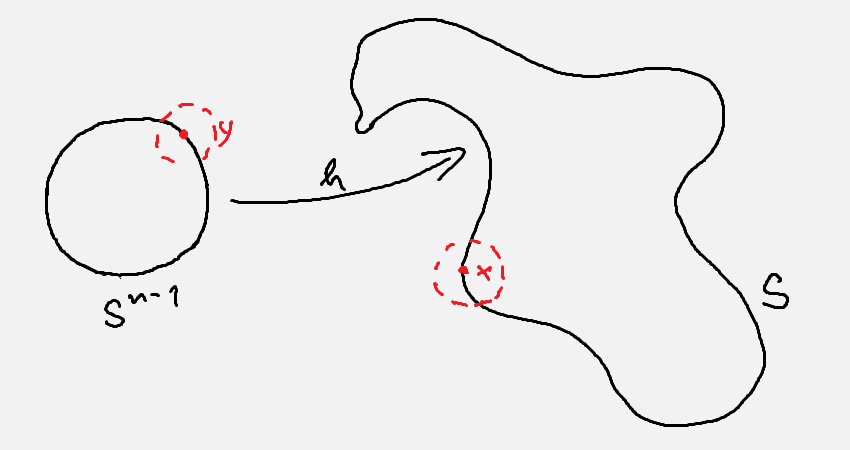
\includegraphics[scale=0.5]{dokaz4.png}
  \end{center}
  Potem je $h^{-1} (W)$ odprta okolica za $y \in S^{n - 1}$ in obstaja $r > 0$, da je 
  $$H := \overline{K(y, r)} \cap S^{n - 1} \subseteq h^{-1} (W)$$ in $G := \overline{S^{n - 1} \setminus H} \cong B^{n - 1}.$
  Po prejšnjem izreku $D := h(G) \cong B^{n - 1}$ ne deli $\R^n$. Naj bo sedaj $V'$ še ena komponenta $\R^n \setminus S$
  in $v' \in V'$. Izberemo še nek $v \in V$. Ker $D$ ne deli $\R^n$, obstaja pot 
  $$\gamma: (I, 0, 1) \to (\R^n \setminus D, v, v').$$
  Ker $v$ in $v'$ pripadata različnim komponentam $\R^n \setminus S$, mora ta pot vsaj nekje sekati $S$ oziroma natančneje 
  $S \setminus D$, ki pa je vsebovana v $W$. Naj bo $t_0$ prva točka, pri kateri je $\gamma (t) \in S$.
  Ker je $$\gamma^{-1} (S)^{\ \text{zap}} \subseteq [0, 1] = I,$$
  res obstaja najmanjša točka v tej množici.
  Torej imamo $\gamma(t_0) \in S \cap W$ in $\gamma\big|_{[0, t_0)}$ slika v $V$.
  Ker je $\gamma$ zvezna, za okolico $W$ točke $\gamma(t_0)$ obstaja $\delta > 0$, da je 
  $\gamma((t_0 - \delta, t_0 + \delta)) \subseteq W$. To pa bi pomenilo, da $\gamma$ interval $(t_0 - \delta, t_0)$
  slikal v $V \cap W$, ki pa je po naši predpostavki iz dokaza prazna množica.
\end{dokaz}

Da ima $\R^n \setminus S$ res natanko dve komponenti, dokazujemo za posebni primer $n = 2$.

\begin{lema}
  Naj bosta $h = (h_1, h_2)$ in $v = (v_1, v_2)$ poti 
  $$h, v: [-1, 1] \to P = [a, b] \times [c, d],$$
  za kateri velja $h_1 (-1) = a$, $h_1 (1) = b$, $v_2 (-1) = c$ in $v_2 (1) = d$.
  Potem se tira poti $h$ in $v$ sekata, torej obstajata $s, t \in [-1, 1]$, da je $h(s) = v(t)$.
  \begin{center}
    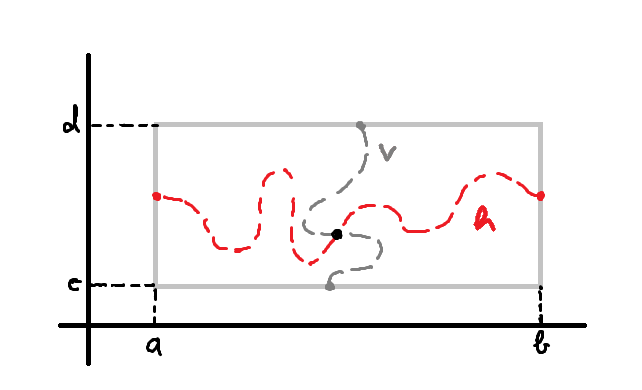
\includegraphics[scale=0.6]{lema1.png}
  \end{center}
\end{lema}

\begin{dokaz}
  Denimo, da trditev ne velja. Potem za vsak $s, t \in [-1, 1]$ velja $h(s) \neq v(t)$.
  Naj bo torej $$D(s, t) := \max \{|h_1 (s) - v_1 (t)|, |h_2 (s) - v_2 (t)|\} > 0,$$
  ki je zvezna preslikava $[-1, 1]^2 \to (0, \infty)$.
  Definiramo preslikavo $f: [-1, 1]^2 \to [-1, 1]^2$ kot 
  $$f(s, t) := \frac{(v_1 (t) - h_1 (s), h_2 (s) - v_2 (t))}{D(s, t)}.$$
  Trdimo, da ta preslikava nima negibne točke. Res, ker je ena od komponent $f$ vedno enaka $\pm 1$, 
  potem $f$ slika v rob kvadrata. Če ima $f$ torej negibno točko, mora ta biti oblike 
  $$(1, t),\quad (-1, t),\quad (s, 1),\quad (s, -1).$$
  Hitro lahko preverimo, da te točke niso negibne, torej smo izpeljali protislovje z izjavo $\mathbf{A_n}$.
\end{dokaz}

\begin{trditev}
  Naj bo $S \subseteq \R^2$ topološka krožnica. Potem ima $\R^2 \setminus S$ natanko eno omejeno komponento. 
\end{trditev}

\begin{dokaz}
  Naj bosta $A$ in $A'$ najbolj oddaljeni točki na $S$ -- ker je metrika $d: S \times S \to [0, \infty)$
  zvezna, na kompaktu vselej zavzame maksimum. Naj torej $d$ zavzame maksimum v $d(A, A') = a$.
  Sedaj izberemo tak koordinatni sistem, da je $A = (0, 0)$ in $A' = (a, 0)$ ter označimo $P := [0, a] \times [-a, a]$.
  Potem je v novem koordinatnem sistemu $S \subseteq P$ in $S \cap \partial P = \{A, A'\}$.
  $A$ in $A'$ razdelita $S$ na dva podloka med $A$ in $A'$ -- ti krivulji ustrezata tiru poti $h$ kot v prejšnji lemi.
  Naj bosta točki $T\left(\frac{a}{2}, a\right)$ in $B\left(-\frac{a}{2}, a\right)$.
  \begin{center}
    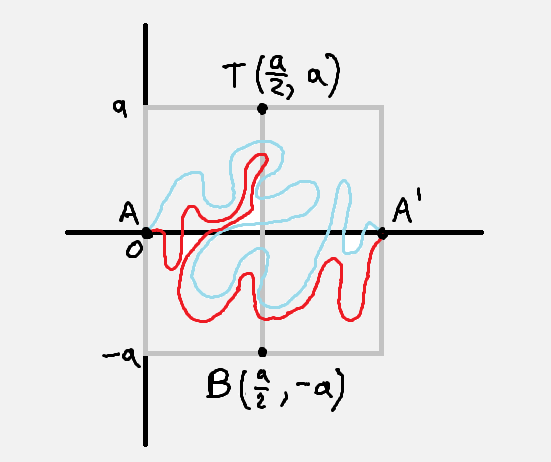
\includegraphics[scale=0.8]{dokaz5.png}
  \end{center}
  Po prejšnji lemi oba loka $S$ sekata daljico $\overline{BT}$.
  Naj bo $M_T$ najvišja točka v preseku $S \cap \overline{BT}$ in označimo s $S_T$ podlok od $A$ do $A'$,
  ki vsebuje $M_T$. Podobno naj bo $m_T$ najnižja točka v $S_T \cap \overline{BT}$. Nato označimo 
  s $S_B$ drugi podlok od $A$ do $A'$ v $S$. Trdimo, da $S_B$ seka $\overline{BT}$ pod $m_T$.
  Sicer vodoravna pot $S_B$ ne bi sekala navpične poti s tirom 
  $$\overline{Bm_T} \cup \text{(podlok $S_T$ od $m_T$ do $M_T$)} \cup \overline{M_T T},$$
  kar je v protislovju z lemo. Naj bo $M_B$ najvišje in $m_B$ najnižje presečišče $S_B$ in $\overline{B m_T}$.
  Označimo s $C$ središče daljice $\overline{M_B m_T}$. Dokazali bomo, da $C$ ne leži v neomejeni komponenti.
  Če bi $C$ bil vsebovan v neomejeni komponenti, potem obstaja $\gamma$ od $C$ do neke točke v 
  komplementu $P$, katere tir ne seka $S$. Naj bo $D$ prva točka, v kateri $\gamma$ seka $\partial P$ in  
  $\gamma_D$ del poti od $C$ do $D$. Denimo, da $D$ leži nad osjo $x$. Potem navpična pot s tirom 
  $$\overline{BC} \cup \gamma_D \cup \text{(po najkrajši poti od $D$ do $T$ znotraj $\partial P$)}$$
  ne seka vodoravne poti $S_T$. Če pa $D$ leži nad osjo $x$, potem navpična pot s tirom 
  $$\text{(najkrajša pot od $B$ do $D$ po $\partial P$)} \cup \gamma_D \cup \overline{C m_T} \cup \text{(podlok v $S_T$ od $m_T$ do $M_T$)} \cup \overline{M_T T}$$
  ne seka vodoravne poti $S_B$ in smo prišli v protislovje.
  Sedaj vemo, da je $C$ v omejeni komponenti (naj bo to $V$), torej ta obstaja. Pokazati moramo še, da je to tudi edina omejena komponenta.
  Če je $V'$ še ena omejena komponenta, potem je $V' \subseteq P$ in ker ima $\R^2 \setminus S$ vsaj 2 komponenti,
  je meja od $V'$ enaka $S$. Naj bo $\gamma_1$ pot s tirom 
  $$\overline{B m_B} \cup \text{(pot v $S_B$ od $m_B$ do $M_B$)} \cup \overline{M_B m_T} \cup \text{(pot v $S_T$ od $m_T$ do $M_T$)} \cup \overline{M_T T}.$$
  $\gamma_1$ potuje po $S \cup V \cup \text{(neomejena komponenta)}$, torej ne seka $V'$.
  Naj bo $r > 0$ tako majhen, da $K(A, r)$ in $K(A', r)$ ne sekata tira $\gamma_1$.
  Ker sta $A, A'$ vsebovana v meji od $V$, potem obstaja $A_1 \in K(A, r) \cap V'$ in 
  $A_1 ' \in K(A_1, r) \cap V'$. Potem pa vodoravna pot s tirom 
  $$\overline{A A_1} \cup \text{(pot v $V'$ od $A_1$ do $A_1'$)} \cup \overline{A_1' A'}$$
  ne seka tira $\gamma_1$ in smo prišli v protislovje.
\end{dokaz}

Naj bo $S \subseteq \R^2$, $S \cong S^1$ in $V$ omejena komponenta $\R^2 \setminus S$. Kaj lahko povemo o topološkem 
tipu $V$ oziroma $\overline{V} = V \cup S$?

\begin{izrek}[Schoenflis]
  Naj bo $S \subseteq \R^2$, $S \cong S^1$ in $V$ omejena komponenta $\R^2 \setminus S$. Potem je $\overline{V} \cong B^2$
\end{izrek}

Denimo, da je $S \subseteq \R^n$, $S \cong S^n$ in $V$ omejena komponenta 
$\R^n \setminus S$. Ali je tedaj $\overline{V} \cong B^{n}$?
Podobno vprašanje si lahko zastavimo tudi za $S \subseteq S^n$, $S \cong S^{n - 1}$. 

\begin{trditev}
  Naj bo $S^{n - 1} \cong S \subseteq \R^n$ in $V$ omejena komponenta $\R^n \setminus S$.
  Potem sta naslednji trditvi ekvivalentni:
  \begin{enumerate}
    \item $\overline{V} \cong B^n$ (Schoenflis)
    \item $\exists$ homeomorfizem $h: \R^n \to \R^n$, tako da je $h(S) = S^{n - 1}$.
  \end{enumerate}
\end{trditev}

\begin{trditev}
  Naj bo $S^{n - 1} \cong S \subseteq S^n$ in $V$ poljubna komponenta $S^n \setminus S$.
  Potem sta naslednji trditvi ekvivalentni:
  \begin{enumerate}
    \item $\overline{V} \cong B^n$.
    \item $\exists$ homeomorfizem $h: S^n \to S^n$, tako da je $h(S) = S^{n - 1}$.
  \end{enumerate}
\end{trditev}

Analogen izrek kot Schoenflisov pa za dimenzijo $n \geq 3$ ne velja brez dodatnih predpostavk.

\begin{figure}[h!]
  \centering
  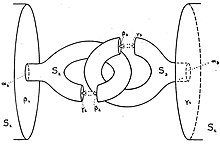
\includegraphics[scale=0.7]{alexander.jpg}
  \caption{Alexandrova rogata sfera}
\end{figure}

Topološke sfere, ki so protiprimeri, so divje v smislu, da imajo točke, v okolici katerih je struktura 
vložene sfere kompleksna. Take točke imenujemo divje točke.
Iz trditve vidimo, da je potreben pogoj za veljavnost Schoenflisovega izreka to,
da je $S$ mogoče v okolici vsake točke nekonstantno zravnati.

\begin{center}
  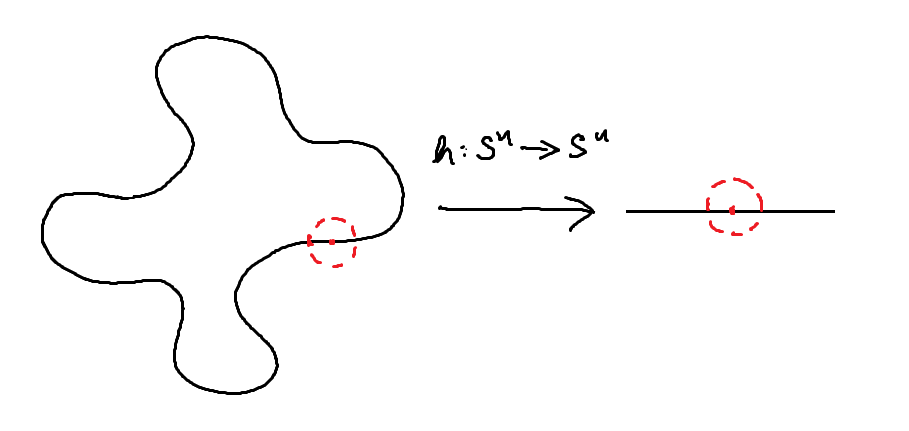
\includegraphics[scale=0.7]{schoenflis1.png}
\end{center}

\begin{definicija}
  \begin{itemize}
    \item Naj bo $S^{n - 1} \cong S \subseteq \R^n$ in $x \in S$. Sfera $S$ je lokalno ploščata ali krotka v točki $x$,
  če obstaja okolica $U \subseteq \R^n$ za $x$ in homeomorfizem $h : U \to W^{\ \text{odp}} \subseteq \R^n$,
  da je $h(S \cap U) = W \cap (\R^{n - 1} \times \{0\})$.
    \item $S$ je lokalno ploščata ali podmnogoterost v $\R^n$, če je lokalno ploščata v vsaki svoji točki.
    \item Točkam, v katerih $S$ ni lokalno ploščata, rečemo divje točke.
  
  \end{itemize}
\end{definicija}

\begin{izrek}
  Schoenflisov izrek velja natanko za lokalno ploščate topološke $(n - 1)$-sfere v $\R^n$ oziroma $S^n$.
\end{izrek}

\begin{figure}[h!]
  \centering
  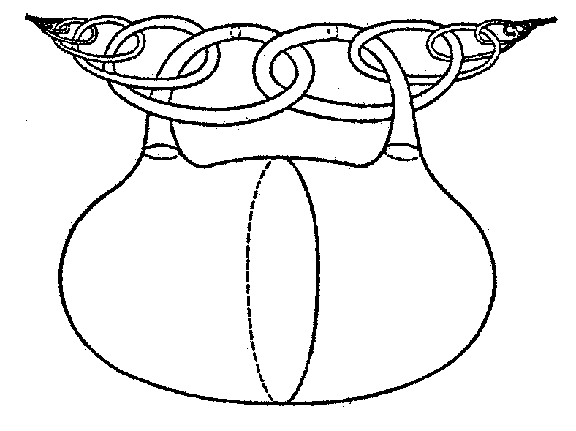
\includegraphics[scale=0.3]{fox-artin.png}
  \caption{Fox-Artinova sfera}
\end{figure}

\subsection{Invarianca odprtih množic}

Cilj tega razdelka je pokazati, da je dimenzija vektorskega prostora $\R^n$ topološka invarianta,
torej če je $\R^n \cong \R^m$, potem sledi $m = n$.
Iz linearne algebre to že vemo za linearne izomorfizme, ki pa so le zelo posebna vrsta homeomorfizmov.
V splošnem pa zvezna preslikava (ne nujno surjektivna) lahko spremeni dimenzijo.

\begin{zgled}
  Oglejmo si nekaj primerov zveznih preslikav, ki ne ohranijo dimenzije prostora.
  \begin{itemize}
    \item Projekcija na prvi faktor iz $\R^2$ v $\R$.
    \item Prostor zapolnjujoče krivulje (Hilbertova, Peanova) iz $I$ v $I^2$.
    \item Prejšnji primer lahko posplošimo na poljubno dimenzijo. Po izreku Aleksandrova obstaja zvezna surjekcija 
    $f: C\to I^n$ in ker je $C^{\ \text{zap}} \subseteq I$, lahko $f$ razširimo na zvezno surjekcijo $f: I \to I^n$.
  \end{itemize}
\end{zgled}

\begin{izrek}[Brouwer]
  Naj bo $U^{\ \text{odp}} \subseteq \R^n$ in $f: U \to \R^n$ zvezna in injektivna. Potem je $f$ odprta vložitev, 
  torej je $f(V)^{\ \text{odp}} \subseteq \R^n$.
\end{izrek}

\begin{dokaz}
  Izberimo poljubno $W^{\ \text{odp}} \subseteq U$ in $y \in f(W)$. Dokazujemo, da ima $y$ odprto okolico v $\R^n$,
  vsebovano v $f(W)$. Zaradi injektivnosti $f$ lahko definiramo $x = f^{-1}(y)$. Za $x \in W^{\ \text{odp}} \subseteq \R^n$
  obstaja $r > 0$, da je $K = \overline{K} (x, r) \subseteq W$ in torej $K \cong B^n$.
  Potem je seveda $\partial K \cong S^{n - 1}$ in $\inte K \cong \mathring{B}^n$.
  Označimo $S = f(\partial K)$ in 
  $$f\big|_{\partial K} : \partial K \to \R^n\ \text{ je zaprta.}$$
  To pa pomeni, da je tudi vložitev, zato je $S \cong S^{n - 1}$. Po 
  Jordan-Brouwerjevem izreku ima $\R^n \setminus S$ dve komponenti, ki sta odprti
  v $\R^n$:
  $$\R^n \setminus S = f(\inte K) \cup (\R^n \setminus f(K)).$$
  Pri tem je $f(\inte K)$ povezana, ker je zvezna slika povezane, $\R^n \setminus f(K)$
  pa je povezana, ker zaradi zaprtosti $f \big|_{K}$ velja $f(K) \cong K \cong B^n$,
  po izreku $\mathbf{D_n}$ pa topološki disk ne deli $\R^n$.
  Torej sta $f(\inte K)$ in $\R^n \setminus f(K)$ komponenti $\R^n \setminus S$
  in zato odprti v $\R^n$.
  Od tod pa naprej 
  $$y = f(x) \in f(\inte K)^{\ \text{odp v $\R^n$}} \subseteq f(W)$$
  in $y$ je notranja točka.
\end{dokaz}

\begin{opomba}
  Pri tem izreku je pomembno, da se nahajamo v ambientnem prostoru $\R^n$.
  V splošnem to seveda ne velja; vzamemo lahko na primer množico $[0, 1) ^{\ \text{odp}} \subseteq [0, \infty)$
  in na njej uporabimo preslikavo $f(x) = x + 1$.
  \begin{center}
    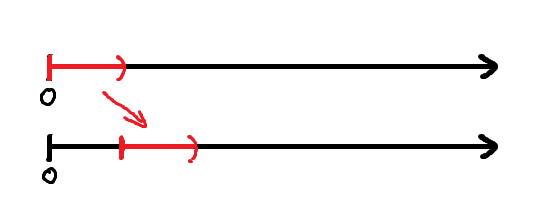
\includegraphics[scale=0.7]{opomba2.png}
  \end{center}
\end{opomba}

\begin{izrek}[Invarianca odprtih množic]
  Naj bo $V^{\ \text{odp}} \subseteq \R^n$ in $W \subseteq \R^n$, tako da je $W \cong V$.
  Potem je $W$ odprta v $\R^n$.
\end{izrek}

\begin{dokaz}
  Po predpostavki obstaja homeomorfizem $h: V \to W$. Sedaj definiramo funkcijo 
  $$f: V \stackrel{h}{\to} W \stackrel{i}{\hookrightarrow} \R^n.$$
  Ker je $f$ zvezna in injektivna, je po izreku $f$ odprta in $f(V) = W^{\ \text{odp}} \subseteq \R^n$.
\end{dokaz}

\begin{posledica}
  Iz $\R^n \cong \R^m$ sledi $n = m$.
\end{posledica}

\begin{dokaz}
  Naj bo $\R^n \cong \R^m$ in denimo, da je $m < n$. 
  Ker je $\R^n$ odprta v $\R^n$, bi po izreku morala biti tudi $\R^m \equiv \R^m \times {0}^{n -m} \subseteq \R^n$
  odprta. To pa je protislovje, saj ima ${0}^{n -m}$ prazno notranjost.
\end{dokaz}

\begin{opomba}
  V splošnem sta notranjost in meja množice odvisna od tega, kako je množica vložena v prostor.
  Kot smo dokazali, pa se to ne zgodi znotraj $\R^n$.
\end{opomba}

\begin{trditev}
  Naj bosta $A, B \subseteq \R^n$ in $h: A \to B$ homeomorfizem.
  Potem je $$h(\inte A) = \inte B,\quad h(A \cap \meja A) = B \cap \meja B.$$
\end{trditev}

\begin{dokaz}
  Ker je ${\inte A}^{\ \text{odp}} \subseteq \R^n$, je $h(\inte A)$ tudi odprta v $\R^n$ in zato 
  vsebovana v $\inte B$, torej $h(\inte A) \subseteq \inte B$.
  Obratna inkluzija za $h^{-1}$ da $h^{-1} (\inte B) \subseteq \inte A$, torej je res $h(\inte A) = \inte B$.
  Druga točka pa sledi zato, ker je $h$ bijekcija.
\end{dokaz}

\clearpage
\section{Mnogoterosti}

\subsection{Topološke mnogoterosti}

Ta razdelek začnimo z intuicijo, da je mnogoterost dimenzije $n$
topološki prostor, ki lokalno "`izgleda"' kot $\R^n$.
Osnovni primeri bi bile krivulje in ploskve, ki jih že poznamo iz analize.
Vnaprej se dogovorimo za oznako $\R^n_+ := \R^{n - 1} \times [0, \infty)$
in $\R^{0} = \{0\}.$

\begin{figure}[htb!]
  \centering
  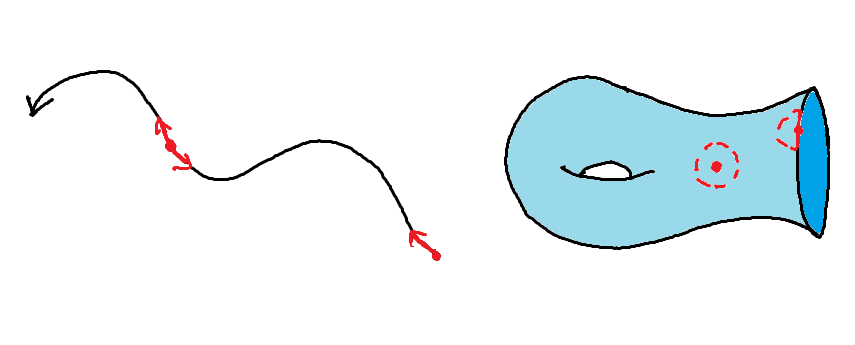
\includegraphics[scale=0.6]{mnogoterost1.png}
  \caption{Primer krivulje in ploskve, osnovnih mnogoterosti.}
\end{figure}

\begin{definicija}
  Naj bo $n \in \N_0$. Topološka mnogoterost dimenzije $n$ oziroma $n$-mnogoterost 
  je $2$-števen Hausdorffov prostor, v katerem ima vsaka točka 
  odprto okolico, homeomorfno $\R^n$ ali $\R^n_+$.
  Takšno okolico imenujemo evklidska okolica, pripadajoč homeomorfizem pa karta.
\end{definicija}

\begin{definicija}
  Točka $x \in X$ je notranja, če ima kakšno okolico, ki je homeomorfna $\R^n$,
  sicer pa je $x$ robna točka. Množico vseh notranjih točk mnogoterosti 
  imenujemo notranjost $X$ in ga označujemo z $\intem X$, preostanek pa imenujemo rob od $X$
  in ga označujemo z $\partial X := X \setminus \intem X$. 
\end{definicija}

\begin{opomba}
  \begin{itemize}
    \item $\R^n \cong \mathring{B}^n$, $\R^n_+ \cong \mathring{B}^n_+ = \mathring{B}^n \cap \R^n _+.$
    Alternativno lahko evklidske okolice definiramo kot tiste, ki so homeomorfne odprtim podmnožicam v $\R^n_+$.
    \item Vsak $x \in X$ ima bazo evklidskih okolic.
    \item V literaturi mnogoterost včasih pomeni mnogoterost brez roba.
  \end{itemize}
\end{opomba}

\begin{zgled}
  \begin{itemize}
    \item $S^1$ je $1$-mnogoterost z notranjostjo $\intem S^1 = S^1$ in robom $\partial S^1 = \emptyset$.
    \item Naj bo $V^{\ \text{odp}} \subseteq X^{\ \text{$n$-mnt.}}$. Potem je tudi $V$ $n$-mnogoterost.
    \item Gladka podmnogoterost (ta pojem poznamo že iz analize) dimenzije $n$ v $\R^m$ je tudi topološka 
    mnogoterost dimenzije $n$.
  \end{itemize}
\end{zgled}

\begin{zgled}
$\R^n$ je $n$-mnogoterost brez roba, $\R^n_+$ pa $n$-mnogoterost z robom $\partial \R^n_+ = \R^{n - 1} \times \{0\}$.
    Če bi $x \in \R^{n - 1} \times \{0\}$ namreč imel okolico $U^{\ \text{odp}}\subseteq \R^n_+$, ki je homeomorfna $\R^n$,
    potem ta $V$ vsebuje $x$, zato $V$ ni odprta v $\R^n$. To pa je v nasprotju z invarianco odprtih množic.  
\end{zgled}
  
\begin{zgled}
  $X = \R \times \{0\} \cup \{0\} \times \R$ ni mnogoterost, saj izhodišče nima evklidske okolice. 
  Če bi jo imela, bi ta ob odstranitvi točke $(0, 0)$ razpadla na vsaj $4$ komponente, kar pa vodi v protislovje.
  Enak argument uporabimo tudi za dokaz, da dvojni stožec $x^2 + y^2 = z^2$ ni mnogoterost.  
  \begin{center}
    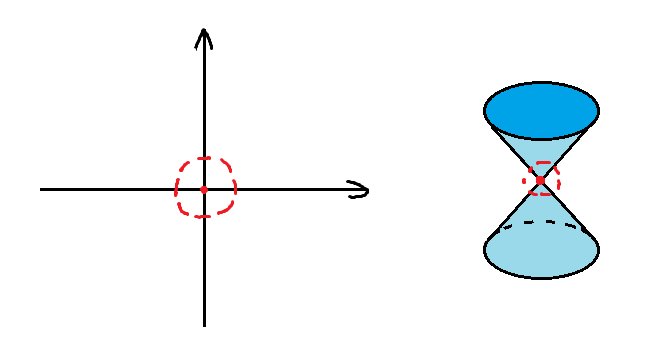
\includegraphics{zgled8.png}
  \end{center}
\end{zgled}

\begin{opomba}
  V primeru sfere vidimo, da notranjost in rob mnogoterosti ne sovpadata nujno z relativno
  notranjostjo in mejo, če je mnogoterost vložena v ambientni prostor.
\end{opomba}

Ker so mnogoterosti lokalno evklidske, imajo enake lokalne lastnosti kot $\R^n$.
To pomeni, da so lokalno povezane s potmi, lokalno kompaktne in $T_1$ (že brez predpostavke).
Lastnost $T_2$ pa ni lokalna -- primer smo že srečali pri kvocientu $$\quot{(-\infty, 0)\times \{0\} \cup [0, \infty)\times \{1\} \cup [0,\infty)\times\{-1\}}{\{(0, 1), (0, -1)\}},$$
ki ima evklidske okolice, a ni $T_2$. Vendar pa nam lokalna kompaktnost v kombinaciji 
z predpostavko $T_2$ da regularnost, ta pa skupaj z $2$-števnostjo implicira metrizabilnost.

\begin{definicija}
  Kompaktno mnogoterost brez roba imenujemo sklenjena ploskev.
\end{definicija}

\begin{zgled} 
    Povezane $1$-mnogoterosti (krivulje) so homeomorfne intervalom 
    ali pa krožnici -- to je edina sklenjena krivulja.
    \begin{center}
      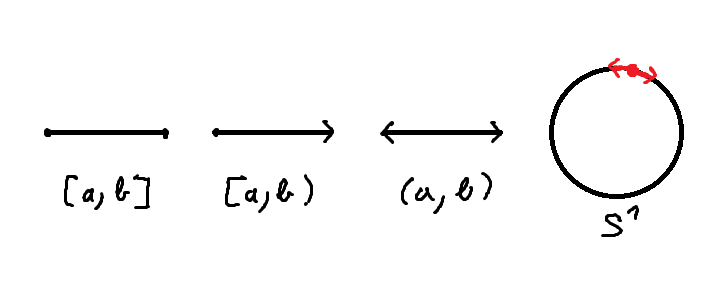
\includegraphics[scale=0.6]{zgled9.png}
    \end{center}
  \end{zgled}

\begin{zgled}
    Povezane kompaktne $2$-mnogoterosti imenujemo ploskve.
    Primeri teh so recimo disk $B^2$, kolobar $S^1 \times I$ ali pa Möbiusov trak.  
    Primeri sklenjenih ploskev pa so Riemannova sfera $S^2 \cong \C P^1$, torus $T = S^1 \times S^1$,
    realna projektivna ravnina $\R P^2 = P$ in Kleinova steklenica.
    \begin{center}
      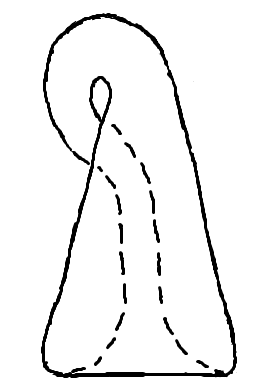
\includegraphics[scale=0.6]{zgled10.png}
    \end{center}
\end{zgled}

\begin{trditev}
  Naj bo $n \in \N_0$ in $\F \in \{\R, \C, \Ha\}$.
  Projektivni prostor $\F P^n$ je sklenjena mnogoterost dimenzije $n$ oziroma $2n$ oziroma $4n$.
\end{trditev}

\begin{dokaz}
   Ker je $q: \F^{n + 1} \setminus \{0\} \to \F P^n$ kvocientna projekcija, je odprta in od tod sledi $2$-števnost.
   Vemo že, da je $\F P^n$ kompakten. Pokazali bomo, da ima vsaka točka odprto okolico,
   ki je homeomorfna $\F^n$, od tod pa bo sledila sklenjenost, lokalna evklidskost in ustrezna dimenzija.
   Za $i = 1, 2, \dots, n + 1$ naj bo $V_i = \{x = (x_1, \dots, x_{n +1}) \in \R^{n + 1} \setminus \{0\}\ |\ x_i \neq 0 \}$
   in $\{V_1, \dots, V_{n + 1}\}$ je odprto pokritje za $\R^{n + 1} \setminus \{0\}$.
   Od tod sledi, da je $\{q(V_1), \dots, q(V_{n + 1})\}$ odprto pokritje za $\F P^n$.
   Dokazali bomo, da je $q(V_i) \cong \F^n$ za vsak $i = 1, \dots, n + 1$.
   Brez škode za splošnost vzemimo $i = 1$ in definirajmo preslikavo $f: V_1 \to \F^n$
   s predpisom $$(x_1, x_2, \dots, x_{n+ 1}) \mapsto (x_1^{-1} x_2, x_1^{-1} x_3,\dots, x_1^{-1}x_{n + 1}).$$
   Hkrati pa je preslikava $q\big|_{V_1}$ kvocientna, saj je zožitev kvocientne preslikave na odprto množico.
   \begin{center}
    \adjustbox{scale=1.5,center}{
      \begin{tikzcd}
        V_1 \arrow[r, "f"] \arrow[d, "q |_{V_1}"']
          & \F^{n} \\
        q(V_1) \arrow[ur, dashed, "\overline{f}"']
          & 
      \end{tikzcd}
    }  
  \end{center} 
  Preslikava $\overline{f}$ obstaja in je zvezna, ker $f$ slika ekvivalenčne 
  razrede v eno točko in je prav tako zvezna.
  Inverz od $\overline{f}$ je $g:\F^{n} \to q(V_1)$, ki je definirana kot
  $g(y_1, \dots, y_n) = q(1, y_1, \dots, y_n)$ in je očitno zvezna.
  Dokazati moramo še, da je $\F P^n$ Hausdorffov prostor.
  Denimo, da imamo točki $a, b \in \F P^n$, kjer je $a := [x] \neq [y] =: b$
  in sta $x, y \in \F^{n + 1} \setminus \{0\}$.
  Če so vse koordinate $x_i \neq 0$, potem je $a \in V(q_i)$ za vse $i = 1, \dots, n + 1$.
  Hkrati pa obstaja neko število $j \in \{1, \dots, n + 1\}$, tako da je 
  $b = [y] \in q(V_j)$ za neki $j$; znotraj $q(V_j) \cong \F^n$ imata $a$ in $b$ disjunktni okolici, ker pa velja
  $q(V_j)^{\ \text{odp}} \subseteq \F P^1$ in zato imata $a$ in $b$ disjunktni odprti okolici v $\F P^n$.
  V splošnem pa po homogenosti obstaja homeomorfizem $h: \F P^1 \to \F P^1$,
  ki preslika $a$ v takšno točko kot prej (torej $x_i \neq 0$, za vsak $i$).
  Po enakem razmisleku imata $h(a)$ in $h(b)$ disjunktni odprti okolici $U$ in $V$,
  torej imata $a$ in $b$ disjunktni odprti okolici $h^{-1} (U)$ in $h^{-1} (V)$.
\end{dokaz}

\subsection{Konstrukcije mnogoterosti}

\begin{enumerate}
  \item \textbf{Komponenta mnogoterosti}
\end{enumerate} 

  Očitno je, da je Hausdorffova in 2-števna, saj sta to dedni lastnosti.
  Ker je mnogoterost lokalno povezana, so njene komponente odprte, od koder pa dobimo tudi
  lokalno evklidskost. Torej je komponenta $n$-mnogoterosti je $n$-mnogoterost.

\begin{enumerate}
  \setcounter{enumi}{1}
  \item \textbf{Disjunktna unija}
\end{enumerate}

Disjunktna unija (največ) števno mnogo $n$-mnogoterosti je prav tako $n$-mnogoterost.

\begin{enumerate}
  \setcounter{enumi}{2}
  \item \textbf{Rob mnogoterosti}
\end{enumerate}

\begin{izrek}[Izrek o odprti preslikavi za mnogoterosti]
  Naj bosta $M$ in $N$ $n$-mnogoterosti, $V^{\ \text{odp}} \subseteq \mathrm{int}\, M$
  in $f: V \to N$ zvezna injektivna funkcija. Potem je $f$ odprta in $f(V) \subseteq \intem N$.
\end{izrek}

\begin{dokaz}
  Izberemo poljubno podmnožico $W^{\ \text{odp}} \subseteq V$, $y \in f(W)$ in $x = f^{-1} (y) \in W$.
  Vemo, da ima $y$ evklidsko okolico $U \subseteq N$, ki je homeomorfna bodisi $\R^n$
  bodisi $\R^n _+$. Potem je $f^{-1} (U)$ okolica za $x$ v $M$ in obstaja evklidska okolica $U'$
  za $x$, tako da je $U' \cong \R^n$ in $U' \subseteq f^{-1} (U) \cap W$.
  Preslikava 
  $$\R^n \stackrel{\cong}{\to} U' \stackrel{f}{\to} U \cong \begin{cases}
    \R^n\\
    \R^n_+
  \end{cases} \stackrel{i}{\hookrightarrow} \R^n$$
  je zvezna in injektivna, zato je po Brouwerjevem izreku odprta.
  Njena slika je odprta podmnožica v $\R^n$,
  zato v primeru $U \cong \R^n _+$ slika ne vsebuje točk iz $\R^{n-1} \times \{0\}$.
  To pa pomeni, da je $y$ notranja točka v $N$, $f(U')^{\ \text{odp}} \subseteq \intem N$ in je znotraj $f(W)$.
\end{dokaz}

\begin{posledica}
  Naj bosta $U, V$ $n$-mnogoterosti in $h: U \to V$ homeomorfizem.
  Potem je $$h(\inte U) = \inte V,\quad h(\partial U) = \partial V.$$
\end{posledica}

\begin{opomba}
  Če je $M$ $n$-mnogoterost, je $\mathrm{int}\, M$ odprta v $M$, zato je $\partial M ^{\ \text{zap}} \subseteq M$.
\end{opomba}

\begin{izrek}
  Naj bo $M$ $m$-mnogoterost z nepraznim robom. Potem je $\partial M$
  $(n - 1)$-mnogoterost s praznim robom. Posebej: če je $M$ kompaktna, je $\partial M$
  sklenjena.
\end{izrek}

\begin{posledica}
  Rob (kompaktne) ploskve je disjunktna unija krožnic.
\end{posledica}

\begin{zgled}
  Naslednja množica ni mnogoterost.
  \begin{center}
    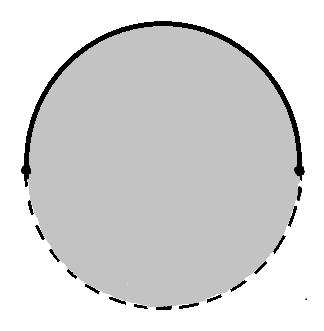
\includegraphics[scale=0.6]{zgled11.png}
  \end{center}
\end{zgled}

\begin{dokaz}
  Po dednosti je $\partial M$ Hausdorffov, 2-števen prostor.
  Za poljuben $x \in \partial M$ trdimo, da ima okolico, homeomorfno
  $\R^{n - 1}$. Naj bo $W$ evklidska okolica za $x$ v $\partial M$,
  $h: W \stackrel{\cong}{\to} \R_+ ^n$ in $h(x) \in \R^{n - 1} \times \{0\}$.
  Po zgornjem izreku $h: W \cap \intem M \to \R_+ ^n$ slika v $\R^{n - 1} \times (0, \infty)$,
  enako $h^{-1}: \R^{n - 1} \times (0, \infty) \to W \cap \intem M$, torej je $h(W \cap \intem M) = \R^{n - 1} \times (0, \infty)$.
  Tako smo dobili iskano karto pri $x$:
  \begin{equation*}
    h\big|_{W \cap \partial M} : W \cap \partial M \to \R^{n - 1} \times \{0\} \equiv \R^{n - 1} \qedhere
  \end{equation*}
\end{dokaz}

\begin{opomba}
  Rob $\partial M$ ne deli $M$: če je $M$ povezana, je $M \setminus \partial M$ povezana.
\end{opomba}

Rob $\partial M$ je lokalno obrobljen v $M$. To pomeni, da če vzamemo $x \in \partial M$,
$x \in W \cong \R^{n - 1} \times [0, \infty)$ in $V := W \cap \partial M$,
je obrobek del $W$, ki ustreza $\R^{n - 1} \times [0, 1]$.

\begin{center}
  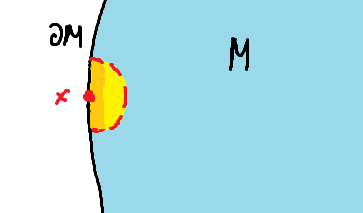
\includegraphics[scale=0.8]{mnogoterost2.png}
\end{center}

\begin{izrek}
  Obstaja vložitev $c: \partial M \times [0, 1] \to M$, da je $c\big|_{\partial M} = id_{\partial M}$.
\end{izrek}

\begin{enumerate}
  \setcounter{enumi}{3}
  \item \textbf{Produkt mnogoterosti}
\end{enumerate}

\begin{trditev}
  Naj bo $M$ $m$-mnogoterost in $N$ $n$-mnogoterost.
  Potem je produkt $M \times N$ $m + n$-mnogoterost z notranjostjo 
  $\intem (M \times N )= \intem M \times \intem N$ in robom 
  $$\partial (M \times N) = \partial M \times N \cup M \times \partial N.$$
\end{trditev}

\begin{dokaz}
  Vemo, da sta lastnosti $T_2$ in 2-števnost produktni.
  Oglejmo si evklidske okolice točk $(x, y) \in M \times N$, kjer je 
  $U_x$ evklidska okolica točke $x \in M$ in $V_y$ evklidska okolica točke 
  $y$ v $N$.
  \begin{itemize}
    \item Če sta $x$ in $y$ notranji, velja $U_x \cong \R^m$, $V_y \cong \R^n$ in 
    $(x, y)$ ima okolico $U_x \times V_y \cong \R^m \times \R^n \equiv \R^{m + n}$,
    zato je notranja točka.
    \item Če je $x \in \intem M$ in $y \in \partial N$, potem je $U_x \cong \R^m$ in $V_y \cong \R^n _+$
    in $$(x, y) \in U_x \times V_y \cong \R^m \times \R^n_+ = \R^{m + n-1} \times [0, \infty) = \R^{m + n}_+.$$
    \item Če je $x \in \partial M$ in $y \in \partial N$, potem je $U_x \cong \R^m$ in $V_y \cong \R^n _+$ in 
    \begin{equation*}
      (x, y) \in U_x \times V_y \cong \R^{m + n - 2} \times [0, \infty)^2 \cong \R^{m + n - 1} \times [0, \infty) = \R^{m + n}_+ \qedhere 
    \end{equation*}
  \end{itemize}
\end{dokaz}

\begin{zgled}
  \begin{itemize}
    \item Kvadrat $I \times I$ je mnogoterost z robom $\partial I \times I \cup I \times \partial I$.
    \item Torus $S^1 \times S^1$ je mnogoterost brez roba, saj ima $S^1$ prazen rob.
    \item Poln torus $S^1 \times B^2$ je mnogoterost z robom $\partial (S^1 \times B^2) = S^1 \times S^1$.
  \end{itemize}
  \begin{center}
    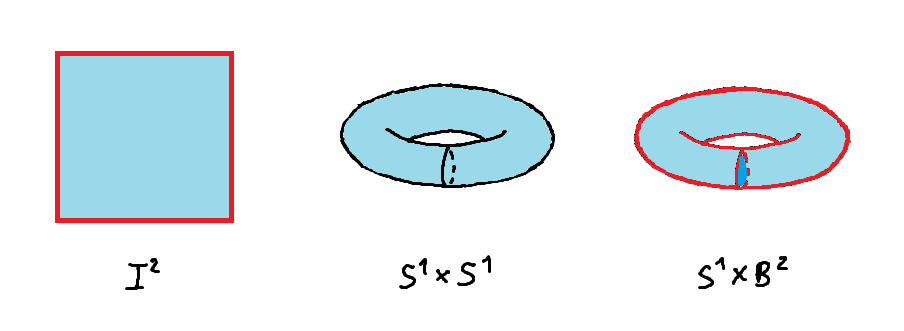
\includegraphics[scale=0.6]{torus.png}
  \end{center}
\end{zgled}

\begin{enumerate}
  \setcounter{enumi}{4}
  \item \textbf{Zlepek mnogoterosti}
\end{enumerate}

\begin{center}
  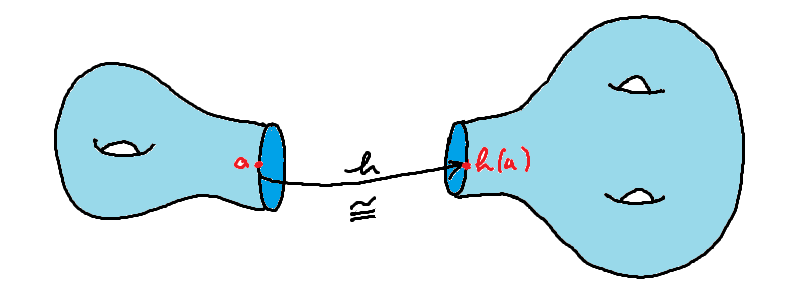
\includegraphics[scale=0.6]{zlepek_mnogoterosti.png}
\end{center}

\begin{definicija}
  Naj bo $L$ $l$-mnogoterost, $N$ $n$-mnogoterost, $L \subseteq N$ in $l \leq n$.
  \begin{enumerate}
    \item Mnogoterost $L$ je prav vložena v $N$, če je $L \cap \partial N = \partial L$.
    \item $L$ je lokalno ploščata ali podmnogoterost v $N$, če je prav vložena in če za vsak $x \in L$
    obstaja neka evklidska okolica $V$ za $x$ v $N$ ter homeomorfizem 
    $$h: V \to \begin{cases}
      \R^n\\
      \R^n_+
    \end{cases},$$
    da je $$h(V \cap L) = h(V) \cap (\{0\}^{n - l} \times \R^{l}).$$
  \end{enumerate}
  \begin{center}
    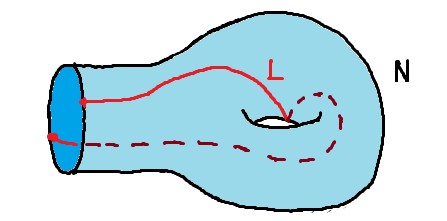
\includegraphics[scale=0.7]{definicija1.png}
  \end{center}
\end{definicija}

\begin{izrek}
  Naj bosta $N_1$ in $N_2$ $n$-mnogoterosti ter $L_1 \subseteq \partial N_1$ in 
  $L_2 \subseteq \partial N_2$ zaprti $(n - 1)$-mnogoterosti z lokalno ploščatima roboma.
  Naj bo $h: L_1 \to L_2$ homeomorfizem. Potem je zlepek $N_1 \cup_h N_2$ $n$-mnogoterost z robom 
  $$\partial (N_1 \cup_h N_2) = (\partial N_1 \setminus \intem L_1) \cup_{h\big|_{\partial L_1}} (\partial N_2 \setminus \intem L_2).$$
\end{izrek}

\begin{dokaz}
  Hausdorffovost in 2-števnost sledita iz trditve \ref{trd:1}.
  Lepljenje na enak način kot v dokazu te trditve pa nam da tudi lokalno evklidskost.
\end{dokaz}

\begin{enumerate}
  \setcounter{enumi}{5}
  \item \textbf{Prerez mnogoterosti}
\end{enumerate}

Naj bo $N$ $n$-mnogoterost in $L^{\ \text{zap}} \subseteq N$ $(n - 1)$-mnogoterost,
ki je lokalno ploščata (in zato seveda tudi prav vložena). Potem $N$ lahko 
prerežemo vzdolž $L$ in dobimo novo $n$-mnogoterost, ki vsebuje po dve kopiji vsake točke iz $L$.
Torej $N \setminus L$ zlepimo s "`polovicami"' okolic notranjih točk v $L$ v $N$ in "`četrtinami"'
okolic robnih točk v $L$ v $N$.

\begin{center}
  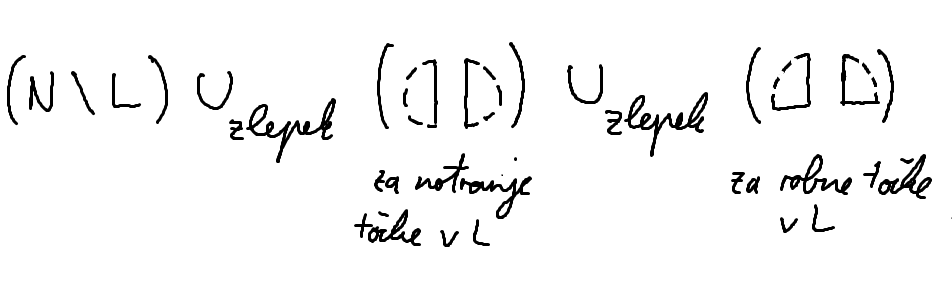
\includegraphics[scale=0.6]{prerez.png}
\end{center}

\begin{zgled}
  Razrez mnogoterosti ponazorimo na Möbiusovem traku, ki ga prerežemo po srednji krivulji. 
  Tako dobimo prostor, ki je homeomorfen $S^1 \times I$, njegova geometrijska realizacija pa je enaka kot v zgledu \ref{zgl:2}.
  Podobno dobimo tudi, če Möbiusov trak razrežemo na tretjini od roba.
  \begin{center}
    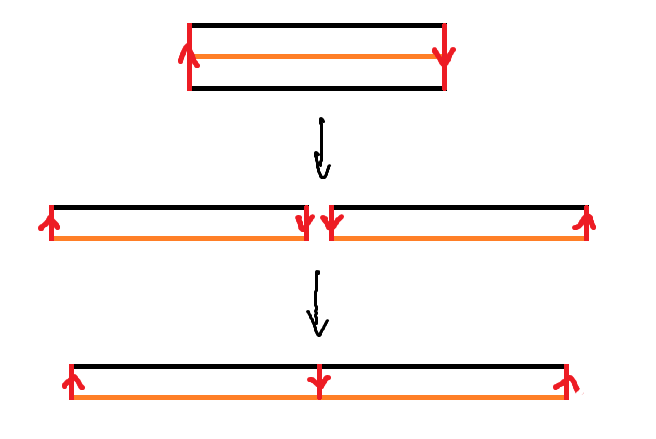
\includegraphics[scale=0.45]{zgled12.png}
  \end{center}
\end{zgled}

\begin{enumerate}
  \setcounter{enumi}{6}
  \item \textbf{Povezana vsota}
\end{enumerate}

\begin{definicija}
  Naj bosta $M, N$ $n$-mnogoterosti, $D \subseteq \intem M$, $E \subseteq \intem N$
  in $D, E \cong B^n$.
  Naj bosta $\partial D \subseteq M$ in $\partial E \subseteq N$ lokalno ploščati sferi
  in $h: \partial D \to \partial E$ homeomorfizem.
  Potem zlepek $M \# N$ imenujemo povezana vsota mnogoterosti $M$ in $N$.
  \begin{center}
    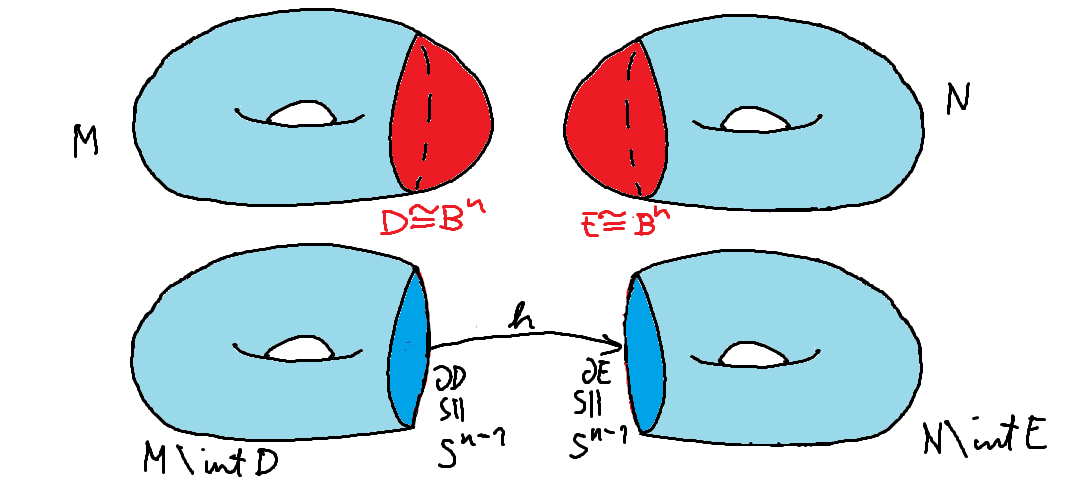
\includegraphics[scale=0.6]{povezana_vsota.png}
  \end{center}
\end{definicija}

Iz konstrukcije razreza in zlepka mnogoterosti sledi, da je $M \# N$ mnogoterost;
zapišemo lahko namreč 
$$M \# N := (M \setminus \intem D) \cup_h (N \setminus \intem E).$$
Kljub temu, da je ta zapis pogosto v uporabi, pa vendarle ni povsem korekten,
saj bi tako definirana mnogoterost lahko bila odvisna od izbire $D$ znotraj iste komponente $M$ 
oziroma izbire $E$ znotraj iste komponente $N$.
Vendar pa se izkaže, da ti izbiri ne vplivata na definicijo -- osnovni rezultat v tej smeri je 
homogenost mnogoterosti. Definicija bi lahko bila odvisna tudi od izbire homeomorfizma $h$. 
Res, dobimo lahko nehomeomorfne rezultate glede na to, ali $h$ ohranja ali obrne orientacijo.
To se lahko zgodi v primeru, ko sta obe mnogoterosti orientabilni in nobena izmed njiju nima
homeomorfizma sama vase, ki bi obrnil orientacijo -- najpreprostejši primer mnogoterosti z zadnjo lastnostjo je $\C P^2$.
Vendar pa je v dveh dimenzijah (torej ploskvah) 
rezultat povezane vsote neodvisen od izbranega homeomorfizma.
V nadaljevanju bomo potrebovali tudi dejstvo, da je povezana vsota sklenjenih ploskev prav tako sklenjena ploskev.

\begin{izrek}[Homogenost mnogoterosti]
  Naj bo $M$ povezana $n$-mnogoterost. Potem za poljubni točki $x, y \in \intem M$ obstaja 
  homeomorfizem $$h: M \to M,\quad h(x) = y.$$
\end{izrek}

\begin{lema}
  Poljuben homeomorfizem $\varphi: S^{n - 1} \to S^{n - 1}$ lahko razširimo do homeomorfizma 
  $\Phi: B^n \to B^n$, ki poljubno vnaprej izbrano točko $x \in \intem B^n$ v poljubno vnaprej izbrano točko 
  $y \in \intem B^n$. 
  \begin{center}
    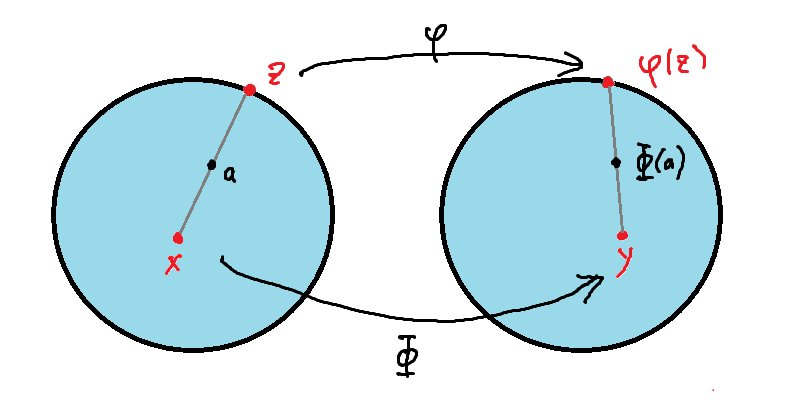
\includegraphics[scale=0.6]{lema2.png}
  \end{center}
\end{lema}

\begin{dokaz}
  Definirajmo ekvivalenčno relacijo na mnogoterosti $M$:
  $$x \sim y \Leftrightarrow \exists\ \mathrm{homeomorfizem}\ h: M \to M,\ h(x) = y.$$
  Dovolj je pokazati, da so vsi ekvivalenčni razredi odprti, saj iz povezanosti $M$
  sledi tudi povezanost $\intem M$. Izberimo $x \in \intem M$
  in naj bo $U$ njegova evklidska okolica, torej $U \stackrel{H}{\cong} \R^n$.
  Definirajmo $V := H^{-1}(\mathring{B^n})$, ki je okolica za $x$, in izberimo poljuben 
  $y \in V.$ Po lemi obstaja homeomorfizem $\Phi: H^{-1} (B^n) \to H^{-1} (B^n)$,
  ki je na robu $H^{-1} (S^{n - 1})$ identiteta in $\Phi(x) = y.$
  Sedaj $\Phi$ razširimo na preostanek $M$ z identiteto in dobimo 
  $x \sim y$ za vsak $y \in V$, torej je ekvivalenčni razred res odprt.
\end{dokaz}

Naj bosta $M, N$ $n$-mnogoterosti, $D \subseteq \intem M$ in $E \subseteq N$ topološka $n$-diska z lokalno ploščatim robom 
ter $h: \partial D \to \partial E$ homeomorfizem. Potem ima operacija 
$$M \# N = (M \setminus \intem D) \cup_h (N \setminus \intem E)$$
nevtralni element. Res, pokazali bomo, da za poljubno $n$-mnogoterost $M$ velja $M \# S^n \cong M$.
Naj bosta $D \subseteq \intem M$, $E \subseteq \intem S^n$ in $\partial E \subseteq S^n$ 
lokalno ploščata $(n - 1)$-sfera, zato po Schoenflisu obstaja homeomorfizem $S^n$, ki $E$
preslika na spodnjo hemisfero $S^n_-$ (in $\partial E$ na ekvator $S^{n - 1} \subseteq S^n$).
Zato smemo privzeti $E = S^n_-$ in $S^n \setminus \mathring{E} = S_+^n \cong B^n$.
Naš homeomorfizem $h: \partial D \to S^{n - 1} = \partial S_+ ^n$ lahko razširimo do homeomorfizma 
$H: D \to S_+^n,$ ki ga definiramo kot $H = \psi^{-1} \circ \tilde{h} \circ \varphi.$ 

  \begin{center}
    \adjustbox{scale=1.1,center}{
      \begin{tikzcd}
        \partial D \ar[rrrrr, "h", bend left=20]
        &
        \subseteq
        &
        D \ar[r, "H", dashed] \ar[d, "\varphi", "\cong"']
        &
        S^n_+ \ar[d, "\psi", "\cong"']
        &
        \supseteq
        &
        S^{n - 1} \\
        S^{n - 1} \ar[rrrrr, "\psi \circ h \circ \varphi^{-1}"', bend right=20]
        & 
        \subseteq 
        &
        B^n \ar[r, "\exists \tilde{h}"', dashed] 
        &
        B^n 
        &
        \supseteq 
        &
        S^{n - 1} 
      \end{tikzcd}
    }
  \end{center}   
S tem pa dobimo naslednji komutativni diagram,
  \begin{center}
    \adjustbox{scale=1.5,center}{
      \begin{tikzcd}
        M
        &
        (M \setminus \mathring{D}) \sqcup D \ar[l] \ar[r, "id \sqcup H"] \ar[d, "q"]
        &
        (M \setminus \mathring{D}) \sqcup S_+^n \ar[d, "p"]
        \\
        &
        (M \setminus \mathring{D}) \cup_{id_{\partial D}} D \ar[ul, dashed, "\cong"', bend left=5]
        \ar[r, dashed, "\cong", "\overline{f}"']
        & (M \setminus \mathring{D}) \cup_h S_+^n \ar[ull, "\cong", bend left=45]
      \end{tikzcd}
    }
  \end{center}   
iz katerega je razvidno, da velja 
$$M \# S^n = (M \setminus \mathring{D}) \cup_h S_+^n \cong M.$$

\subsection{Sklenjene ploskve}

Za nas bo ploskev povezana 2-mnogoterost.
V tem razdelku se bomo ukvarjali s klasifikacijo sklenjenih ploskev,
torej kompaktnih ploskev brez roba.
Našli bomo po enega predstavnika vsakega homeomorfnega razreda 
sklenjenih ploskev in algoritem za njihovo prepoznavanje.

\begin{zgled}
  Primeri sklenjenih ploskev, s katerimi smo se že srečali,
  so sfera $S^2$, torus $T := S^1 \times S^1$, projektivno ravnino 
  $P := \R P^2$ in Kleinova steklenica $K$.
  Iz teh pa lahko konstruiramo vedno nove ploskve.
  \begin{center}
    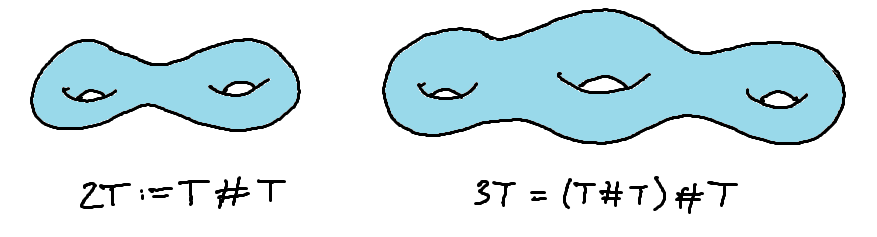
\includegraphics[scale=0.7]{zgled13.png}
  \end{center}
\end{zgled}

Pri tem pa se nam poraja vprašanje, ali s tem dobimo vse sklenjene ploskve in katere izmed njih 
so homeomorfne. Zanimale nas bodo ploskve, ki so kvocienti mnogokotnikov, pri katerih zlepimo 
pare stranic s homeomorfizmi. V primeru $n = 2$ dobimo sfero ali pa projektivno ploskev.
\begin{center}
  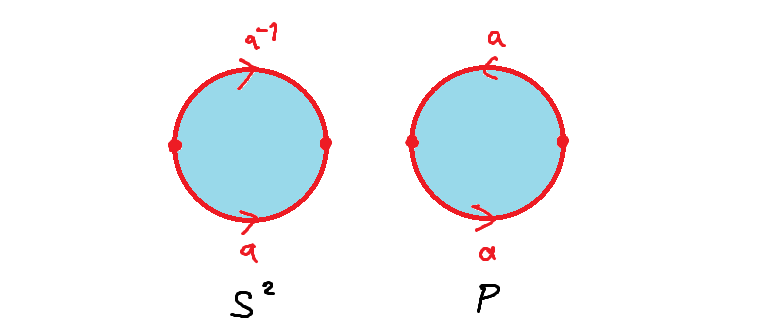
\includegraphics[scale=0.7]{ploskve1.png}
\end{center}
V primeru $n = 3$ je razvidno, da ne dobimo sklenjene ploskve, 
saj z lepljenjem para stranic preostane ena stranica, ki postane rob kvocienta.
Če pa skupaj zlepimo več kot dve stranici, sploh ne dobimo mnogoterosti.
\begin{center}
  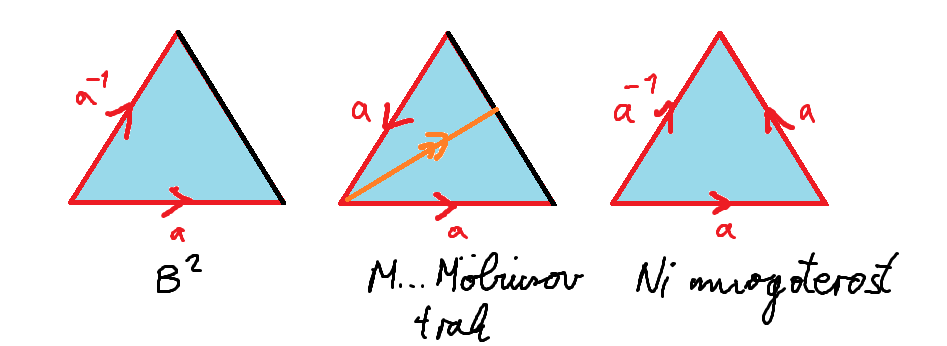
\includegraphics[scale=0.6]{ploskve2.png}
\end{center}
Splošen nauk tega je, da če stranice označujemo 
z množico oznak $A = \{a, b, c, d, \dots\}$, mora vsak 
izmed njenih elementov nastopati dvakrat ali pa nobenkrat.
Te oznake, skupaj z njihovo orientacijo, sestavljajo besedo 
$a^{\varepsilon_1} b^{\varepsilon_2} c^{\varepsilon_3} \dots$,
po kateri zlepimo večkotnik.

\begin{center}
  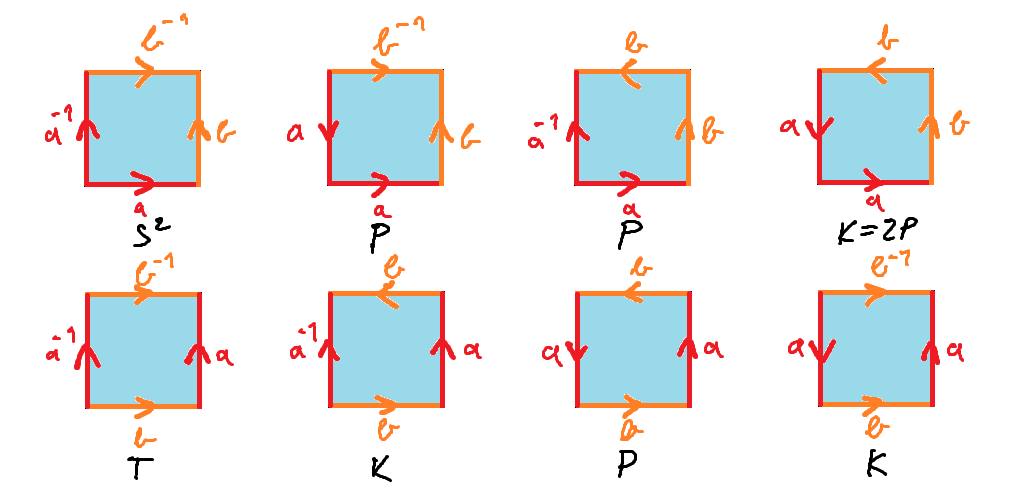
\includegraphics[scale=0.50]{ploskve3.png}
\end{center}

\begin{trditev}
  Naj bo $K = K_1 \sqcup K_2 \sqcup \dots \sqcup K_n$ disjunktna unija mnogokotnikov v ravnini
  in naj bo $\sim$ ekvivalenčna relacija na $K$, ki identificira pare stranic 
  mnogokotnikov z linearnimi homeomorfizmi.
  Potem je $\quot{K}{\sim}$ disjunktna unija kompaktnih ploskev.
  \begin{itemize}
    \item Točke iz notranjosti mnogokotnikov so notranje.
    \item Če je $x$ notranja točke neke stranice, ki se identificira z neko drugo stranico,
    je $[x]$ v $\quot{K}{\sim}$ notranja točka.
    \item Točke iz stranic, ki niso identificirane, so robne.
    \item Ekvivalenčni razredi oglišč lahko vsebujejo več točk.
  \end{itemize}
  Tako ploskev imenujemo poliedrska ploskev.
\end{trditev}

\begin{dokaz}
  Okolice točk v $\quot{K}{\sim}$ dobimo na analogen način kot 
  v dokazu trditve \ref{trd:1}. Od tod sledi tudi to,
  da je $\quot{K}{\sim}$ Hausdorffov in 2-števen, torej moramo 
  preveriti le obstoj evklidskih okolic.
  Pa naredimo to le za primer, ko je $x$ oglišče $K_i$.
  Identifikacije $x$ sledijo iz identifikacije stranic; privzemimo 
  $[x] = \{x, x_1, \dots, x_k\}$. Nato najdemo "`kompatibilne"'
  okolice teh oglišč v $K$, ki so paroma disjunktne.
  \begin{center}
    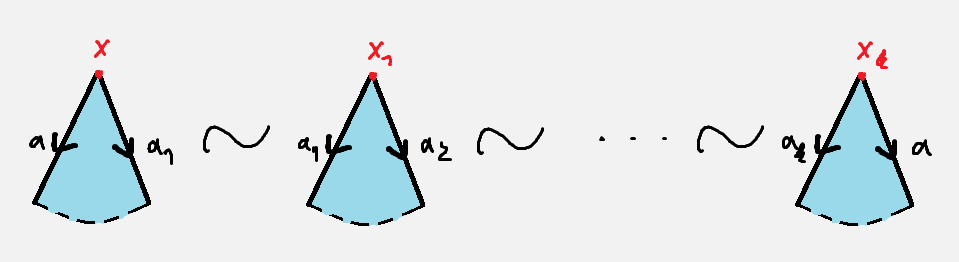
\includegraphics[scale=0.7]{dokaz6.png}
  \end{center}
  Tako nastopita dva primera: z obkroženo in brez obkrožene identifikacije.
  \begin{center}
    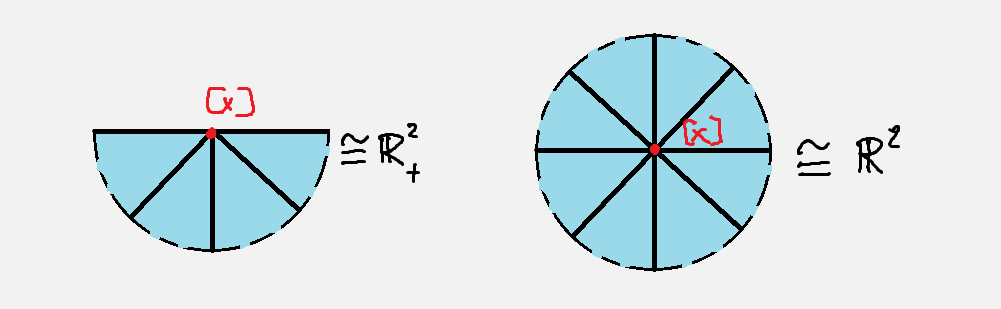
\includegraphics[scale=0.6]{dokaz7.png}
  \end{center}  
\end{dokaz}

Poliedrska ploskev $\quot{K}{\sim}$
ima lahko več komponent. Če pa je povezana, potem pa lahko v $K = \bigsqcup K_i$
najdemo mnogokotnik s stranicami, vzdolž katerih paroma zlepimo komponente tako, da 
nastane en sam mnogokotnik.
Poliedrske ploskve bomo prepoznali s pomočjo dveh topoloških invariant -- lastnosti,
ki se ohranjajo pri homeomorfizmih: orientabilnosti in Eulerjeve karakteristike.
Najprej pa omenimo 

\begin{izrek}[Rádo, 1925]
  Vsaka sklenjena ploskev je homeomorfna neki poliedrski ploskvi.
\end{izrek}

Ta izrek nam zagotovi, da lahko ti invarianti
uporabimo na katerikoli sklenjeni ploskvi. Dokaz izpustimo
\footnote[3]{glej: Strle, S.: Izbrane teme iz geometrijske topologije.}.

\begin{izrek}[Klasifikacijski izrek]
  Naj bo $M$ poljubna poliedrska ploskev, potem je $M$ homeomorfna eni od ploskev 
  $S^2 =: 0 \cdot T$, $nT$ ali $nP$ za nek $n \in \N$,
  zgornje ploskve pa med sabo niso homeomorfne.
\end{izrek}

Povezano vsoto $n$ torusov dobimo tako, da iz vsake kopije torusa 
izrežemo odprt disk in zlepimo robova.
Iz skice vidimo, da je $2T$ kvocient osemkotnika po kvocientu 
$$a_1 b_1 a_1^{-1} b_1^{-1} a_2 b_2 a_2^{-1} b_2^{-1}.$$
\begin{center}
  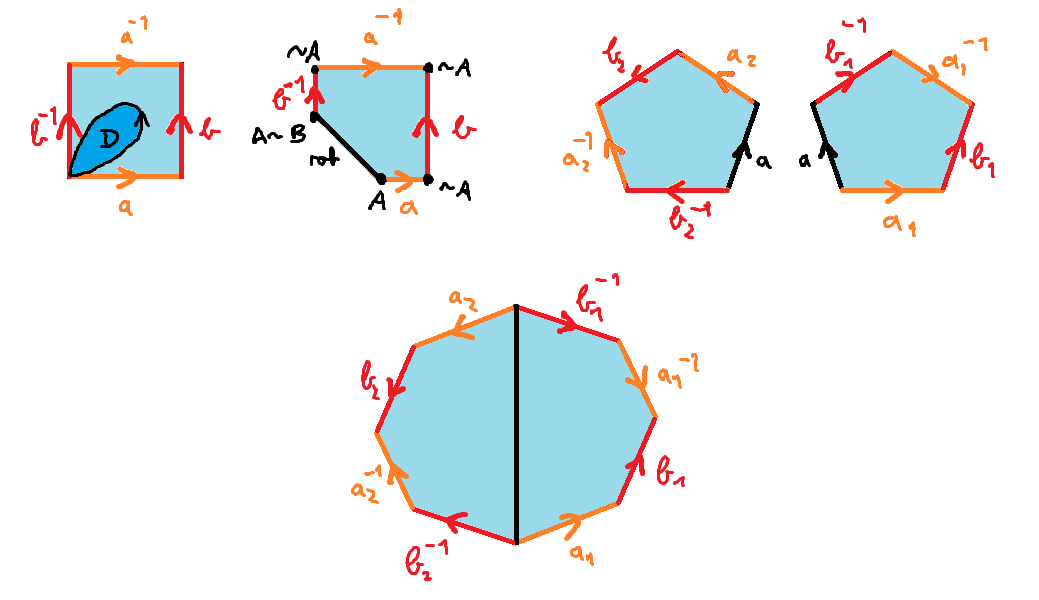
\includegraphics[scale=0.8]{ploskve4.png}
\end{center}
Če to induktivno nadaljujemo, dobimo, da je $nT$
kvocient $4n$-kotnika z besedo 
$$a_1 b_1 a_1^{-1} b_1^{-1} a_2 b_2 a_2^{-1} b_2^{-1} \dots a_n b_n a_n^{-1} b_n^{-1}.$$
Podobno je $2P$ kvocient štirikotnika z besedo $a_1 a_1 a_2 a_2$ in 
induktivno je $nP$ kvocient $2n$-kotnika z besedo 
$$a_1 a_1 a_2 a_2 \dots a_n a_n.$$ 


\begin{enumerate}
  \item \textbf{Orientabilnost}
\end{enumerate}

Mnogokotnik $K \subseteq \R^2$ je orientabilen,
njegova orientacija pa je dana s cikličnim zaporedjem njegovih oglišč.
\begin{center}
  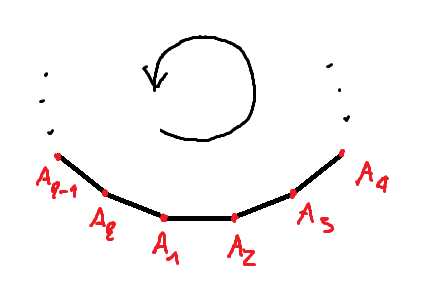
\includegraphics[scale=0.8]{orientabilnost1.png}
\end{center}
Ta določa smer obhoda po $\partial K$ oziroma smer rotacije na $K$.
Hkrati to določa tudi orientacije stranic $K$, ki jih usmerimo skladno s cikličnim 
zaporedjem stranic.

\begin{opomba}
  Orientacija je v tem primeru podana z izbiro zunanje normale 
  na $K \subseteq \R^2 \equiv \R^2 \times \{0\} \subseteq \R^3$
  po pravilu desnega vijaka.
\end{opomba}

Včasih se namesto orientacije govori o "`strani"'
ploskve ali mnogokotnika, ki je tista, kamor kaže normala.
Če sta orientirana mnogokotnika $K_1$ in $K_2$
zlepljena preko neke stranice, potem rečemo, da sta orientirana skladno,
če v skupni stranici določata skladni orientaciji.

\begin{center}
  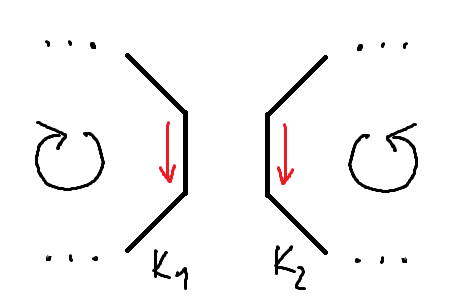
\includegraphics[scale=0.75]{orientabilnost2.png}
\end{center}

\begin{definicija}
  Naj bo $M = \quot{\left(\sqcup_{j = 1}^k K_j\right)}{\sim}$
  poliedrska ploskev, predstavljena kot kvocient disjunktne unije mnogokotnikov,
  v katerih identificiramo nekatere pare stranic s homeomorfizmi.
  $M$ je orientabilna, če lahko orientacije mnogokotnikov $K_j$
  izbiramo tako, da so ti orientirani skladno glede na vsak identificiran par.
\end{definicija}

\begin{zgled}
  Projektivna ravnina $P$ ni orientabilna.
  \begin{center}
    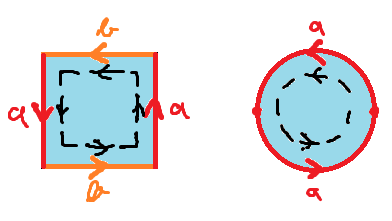
\includegraphics[scale=0.8]{zgled14.png}
  \end{center}
\end{zgled}

Definicija orientabilnosti je odvisna od poliedrske strukture ploskve,
torej predstavitev ploskve kot kvocienta disjunktne unije mnogokotnikov.
Takih predstavitev pa je več -- če hočemo, da je orientabilnost ploskve sploh dobro definirana,
se mora ohranjati s homeomorfizmom.

\begin{izrek}
  Orientabilnost poliedrske ploskve je topološka lastnost.
\end{izrek}

\begin{trditev}
  \begin{enumerate}
    \item Naj bo $M$ poliedrska ploskev in $N$ njena poliedrska 
  podploskev. Potem je tudi $N$ orientabilna.
    \item Če sta $M$ in $N$ orientabilni poliedrski ploskvi,
    je tudi $M \# N$ orientabilna.
  \end{enumerate}
\end{trditev}

\begin{center}
  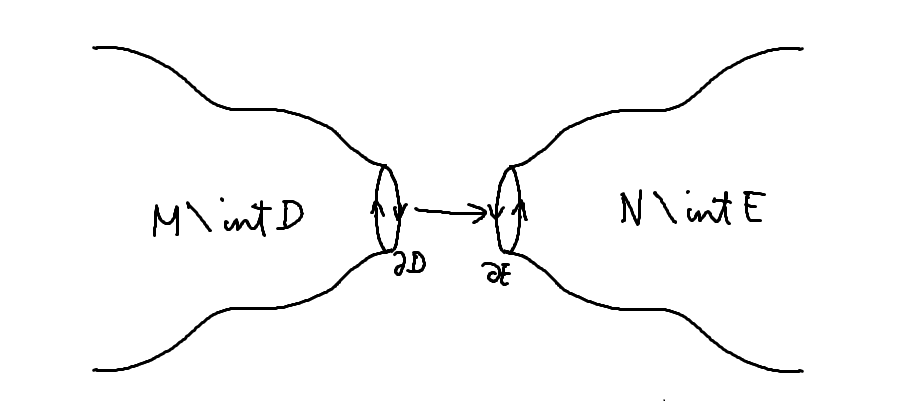
\includegraphics[scale=0.6]{orientabilnost3.png}
\end{center}

\begin{posledica}
  Ploskev $M$ je neorientabilna natanko tedaj, ko vsebuje Möbiusov trak.
\end{posledica}

\begin{zgled}
  Za vsak $n \in \N$ je $nT$ orientabilna, $nP$
  pa neorientabilna ploskev.
\end{zgled}

\begin{enumerate}
  \setcounter{enumi}{1}
  \item \textbf{Eulerjeva karakteristika}
\end{enumerate}

Naj bo $M = \quot{\left(\bigsqcup_{j = 1} K_j\right)}{\sim}$, kjer relacija 
$\sim$ paroma identificira nekatere stranice mnogokotnikov $K_j$.
Unija stranic in oglišč mnogokotnikov določa graf $\Gamma$ v $M$:
oglišča so slike oglišč, povezave so slike stranic, lica grafa pa so slike mnogokotnikov.
\begin{itemize}
  \item \textbf{2-celice} v $M$ so slike odprtih mnogokotnikov $K_j$ v $M$ (torej lica grafa $\Gamma$).
  \item \textbf{1-celice} v $M$ so slike odprtih stranic mnogokotnikov (torej povezave grafa $\Gamma$).
  \item \textbf{0-celice} v $M$ so slike oglišč mnogokotnikov (torej vozlišča grafa $\Gamma$).
\end{itemize}

\begin{definicija}
  Eulerjeva karakteristika $M$ je definirana kot 
  $$\chi (M) = \# (\text{2-celic}) - \# (\text{1-celic}) + \#(\text{0-celic}).$$
\end{definicija}

\begin{trditev}
  Eulerjeva karakteristika sfere je neodvisna od poliedrske strukture in je enaka $\chi(S^2) = 2$. 
\end{trditev}

\begin{dokaz}
  Vemo, da za povezan ravninski graf $\Gamma \subseteq \R^2$ velja 
  $$\# \mathrm{lic} - \# \mathrm{povezav} + \# \mathrm{vozlišč} = 2.$$
  Za dokaz glej diskretno matematiko. Nato opazimo, da lahko graf 
  ravninsko vložimo natanko tedaj, ko ga lahko vložimo brez sekanja stranic na sfero $S^2$ -- uporabimo kar stereografsko 
  projekcijo. S tem pa je trditev že dokazana.
\end{dokaz}

\begin{izrek}
  Eulerjeva karakteristika ploskve $M$ je topološka invarianta, torej je neodvisna od izbire poliedrske strukture na $M$.
\end{izrek}

\begin{opomba}
  Eulerjevo karakteristiko lahko definiramo na končnem CW-kompleksu $(X, \mathcal{E})$\footnote[4]{glej: Mrčun, J.: Topologija}
  kot $$\chi(X) = \sum_{n = 0} ^\infty (-1)^n \# \mathcal{E}_n.$$
  Zgornji izrek velja v splošnem, saj je to število odvisno le od topološkega prostora in ne od celične dekompozicije $\mathcal{E}$:
  dva končna CW-kompleksa, ki sta homeomorfna kot topološka prostora, imata enako Eulerjevo karakteristiko.
\end{opomba}

\begin{zgled}
  Z Eulerjevo karakteristiko lahko sedaj karakteriziramo naše tri družine sklenjenih ploskev.
  \begin{itemize}
    \item $\chi(S^2) = 1 - 1 + 2 = 2$.
    \item $\chi(nT) = 1 - 2n + 1 = 2 - 2n$.
    \item $\chi(nP) = 1 - n + 1 = 2 - n$.
  \end{itemize}
\end{zgled}

\begin{opomba}
  V splošnejši definiciji Eulerjeve karakteristike velja $\chi(S^n) = 1 + (-1)^n$.
\end{opomba}

\begin{trditev}
  Naj bo $M$ poliedrska ploskev in $A, B \subseteq M$ uniji celic,
  tako da je $M = A \cup B$. Potem je 
  $$\chi(M) = \chi (A \cup B) = \chi (A) + \chi(B) - \chi(A \cap B).$$
\end{trditev}

Za dokaz klasifikacijskega izreka moramo še pokazati,
da je vsaka sklenjena ploskev homeomorfna $S^2$, $nT$ ali pa $nP$
za nek $n \in \N$. Naj bo $M$ poljubna poliedrska sklenjena ploskev.
Potem je $M$ povezana, zato jo lahko predstavimo kot kvocient nekega 
mnogokotnika, določenega z neko besedo.

\begin{center}
  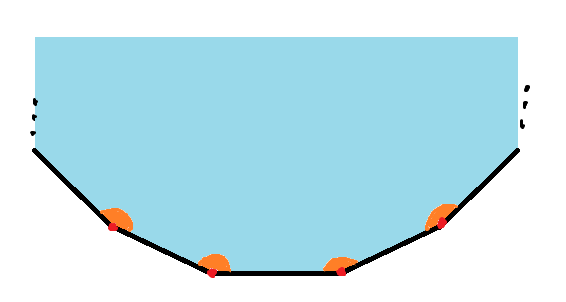
\includegraphics[scale=0.7]{klasifikacija1.png}
\end{center}

Privzeti smemo, da je $M$ kvocient nekega pravilnega mnogokotnika,
v katerem se pari stranic zlepijo z linearnimi homeomorfizmi.
Naj bo $\varepsilon > 0$ dovolj majhen, da so zaprti krogi 
okoli oglišč s polmerom $\varepsilon$ paroma disjunktni.
Ploskev $M$ prerežemo vzdolž teh krogov, torej definiramo 
$$N := \quot{M}{\textup{unija odprtih $\varepsilon$-krogov okoli vseh oglišč}}.$$
Preostanek tvorijo slike teh krogov v $M$; slike zaprtih krogov
se v $M$ zlepijo v zaprte diske s središči v slikah vozlišč.
Tako definiran prostor $N$ je kompaktna ploskev z robom -- na te se prilepijo 
diski, tako da tvorijo sklenjeno ploskev $M$. Oglejmo si primer na torusu.

\begin{center}
  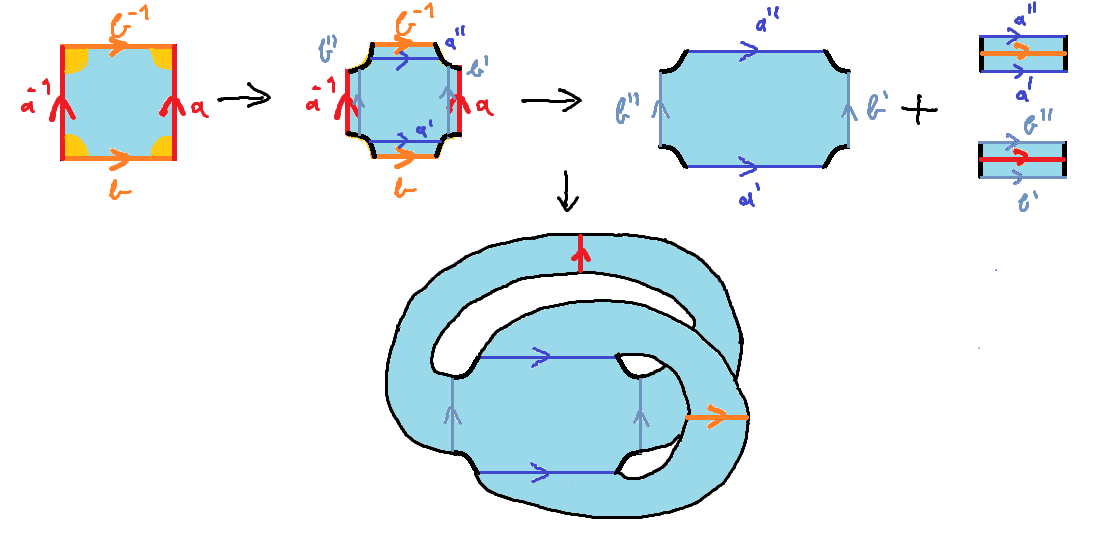
\includegraphics[scale=0.8]{klasifikacija2.png}
\end{center}

\begin{opomba}
  Če bi enak postopek ponovili na projektivni ravnini $P$,
  bi dobili Möbiusov trak.
\end{opomba}

Torus z izrezanim diskom bi si lahko predstavljali kot disk, na katerega 
prilepimo par prepletenih ročajev.

\begin{center}
  \includegraphics[scale=0.6]{klasifikacija3.png}
\end{center}

V splošnem lahko ploskev $N$ predstavimo kot disk s prilepljenimi trakovi,
ki jih imenujemo ročaji.
Ročaj je orientabilen, če je unija diska in ročaja kolobar oziroma je 
homeomorfna $S^1 \times I$.
V nasprotnem primeru pa je ročaj neorientabilen in tedaj je unija diska in 
ročaja homeomorfna Möbiusovemu traku.
Iz ploskve $N$ spet dobimo nazaj začetno ploskev $M$,
tako da na njene robne komponente prilepimo diske.
Od tod naprej ločimo dva primera.

\begin{enumerate}
  \item \textbf{Vsi ročaji so orientabilni.}
\end{enumerate}

V tem primeru lahko vedno izoliramo prepletene
pare ročajev.

\begin{center}
  \includegraphics[scale=0.7]{klasifikacija4.png}
\end{center}

Neprepleteni ročaji določajo robne krožnice, na katere lahko prilepimo po robu diske.
Tako lahko vse neprepletene ročaje odstranimo.
Prepleteni pari pa so opisani z besedo $aba^{-1}b^{-1}$,
ki ustreza enemu torusu. Število prepletenih parov (označimo ga z $n$) torej ustreza številu torusov v povezani vsoti.
Tako velja $M \cong nT$.

\begin{enumerate}
  \setcounter{enumi}{1}
  \item \textbf{Obstaja neorientabilen ročaj.}
\end{enumerate}

\begin{center}
  \includegraphics[scale=0.7]{klasifikacija5.png}
\end{center}

Take ročaje lahko vedno izoliramo od ostalih.
Vsak prepleten par lahko s pomočjo enega neorientabilnega ročaja
spremenimo v tri ločene neorientabilne ročaje.
Od tod sledi $M \cong nP$.

\begin{opomba}
  $P \# T \cong 3P$.
\end{opomba}

\end{document}





